% Anonymous ICLR 2027 manuscript. Build with ./build.sh. Numerical tables are generated.
\documentclass{article}
\usepackage{iclr2027_conference,times}

\usepackage[utf8]{inputenc}
\usepackage[T1]{fontenc}
\usepackage{amsmath,amssymb,amsfonts}
\usepackage{graphicx}
\usepackage{booktabs}
\usepackage{multirow}
\usepackage{array}
\usepackage{xcolor}
\usepackage{tikz}
\usetikzlibrary{positioning,arrows.meta,calc,fit,backgrounds,shapes.geometric}
\usepackage{caption}
\captionsetup{font=small,labelfont=bf}
\usepackage{hyperref}
\hypersetup{hidelinks}
\usepackage{url}
\usepackage{microtype}
\usepackage{placeins}
\usepackage{float}
\usepackage{enumitem}
\setlist{nosep,leftmargin=*}

\graphicspath{{figures/}}
% macros.tex -- notation for the NM-ROM methods section.
% Symbol conventions (kept deliberately disjoint from the old submission, which
% overloaded K for both the discrete operator and a latent-adjacent quantity):
%   N  intervals per axis        n  interior unknowns
%   R  spatial bank width        k  latent dimension
%   M  number of retained weak tests    m  number of empirical-quadrature nodes

\newcommand{\Real}{\mathbb{R}}
\newcommand{\Nat}{\mathbb{N}}

% --- discrete objects -------------------------------------------------------
\newcommand{\Aop}{A}                    % fixed linear discrete operator
\newcommand{\bank}{G}                   % frozen spatial bank, n x R
\newcommand{\head}{h_\theta}            % nonlinear coefficient map, R^k -> R^R
\newcommand{\tests}{P}                  % weak test matrix, M x n
\newcommand{\rowscale}{\Lambda}         % diagonal row scaling
\newcommand{\lift}{u_{g}}               % boundary lift
\newcommand{\bcmask}{\mu}               % boundary mask / vanishing factor
\newcommand{\latent}{z}
\newcommand{\umanifold}{u}

% --- operators and norms ----------------------------------------------------
\newcommand{\jac}[1]{J_{#1}}
\newcommand{\dhead}{D\head}
\newcommand{\norm}[1]{\lVert #1 \rVert}
\newcommand{\normF}[1]{\lVert #1 \rVert_{F}}
\newcommand{\inner}[2]{\langle #1, #2 \rangle}
\newcommand{\T}{^{\top}}
\newcommand{\Tr}{\operatorname{tr}}
\newcommand{\diag}{\operatorname{diag}}
\newcommand{\rank}{\operatorname{rank}}
\newcommand{\argmin}{\operatorname*{arg\,min}}

% --- residuals --------------------------------------------------------------
\newcommand{\rfull}{r}                  % full discrete residual
\newcommand{\rweak}{r_{w}}              % weak (projected, row-scaled) residual
\newcommand{\station}[2]{\eta(#1,#2)}   % normalized-gradient stationarity measure

% --- placeholders for generated numbers -------------------------------------
% Every numeric value in this manuscript must come from a generator script that
% reads the run JSONs. \todo marks a slot that the generator has not yet filled.
\newcommand{\todo}[1]{{\color{red}\textbf{[\,#1\,]}}}
\newcommand{\gen}[1]{\todo{from generator: #1}}

% Subscripted variants (the base macros already carry a subscript, so
% \head_a / \rweak_n would be a double subscript).
\newcommand{\headc}[1]{h_{\theta,#1}}   % one component of the head output
\newcommand{\rweakn}[1]{r_{w,#1}}       % the weak residual of time step #1

% GENERATED by paper/gen_tables.py -- do not edit.
% Every prose number in the manuscript is one of these macros.
\newcommand{\nAblBurgersBestFound}{2.5447}
\newcommand{\nAblBurgersFloor}{0.3918}
\newcommand{\nAblBurgersFree}{0.6027}
\newcommand{\nAblBurgersFreeMs}{2417.6}
\newcommand{\nAblBurgersLinear}{56.9296}
\newcommand{\nAblBurgersNeural}{2.5629}
\newcommand{\nAblBurgersNeuralMs}{47.6}
\newcommand{\nAblBurgersPodOneTwentyEight}{10.1198}
\newcommand{\nAblBurgersPodOneTwentyEightMs}{328.3}
\newcommand{\nAblBurgersPodSixteen}{61.6503}
\newcommand{\nAblBurgersQuad}{31.8276}
\newcommand{\nAblBurgersReductionOverFloor}{6.5}
\newcommand{\nAblBurgersSolverGapPp}{0.018}
\newcommand{\nAblPoissonBestFound}{6.0926}
\newcommand{\nAblPoissonDst}{0.0007}
\newcommand{\nAblPoissonDstMs}{4.341}
\newcommand{\nAblPoissonFloor}{2.3148}
\newcommand{\nAblPoissonFree}{2.3274}
\newcommand{\nAblPoissonLinear}{17.2966}
\newcommand{\nAblPoissonNeural}{6.0927}
\newcommand{\nAblPoissonNeuralMs}{5.843}
\newcommand{\nAblPoissonPodOneTwentyEight}{4.3452}
\newcommand{\nAblPoissonPodOneTwentyEightMs}{5.930}
\newcommand{\nAblPoissonPodSixteen}{20.0548}
\newcommand{\nAblPoissonQthirtytwo}{4.6670}
\newcommand{\nAblPoissonQthirtytwoMs}{7.317}
\newcommand{\nAblPoissonQuad}{16.6303}
\newcommand{\nColdCapEightNearest}{6.09}
\newcommand{\nColdCapEightZero}{30.03}
\newcommand{\nColdCapTwelveNearest}{6.09}
\newcommand{\nColdCapTwelveZero}{6.09}
\newcommand{\nColdCapTwoNearest}{6.80}
\newcommand{\nColdCapTwoZero}{91.88}
\newcommand{\nColdConvNearest}{6.09}
\newcommand{\nColdConvZero}{6.09}
\newcommand{\nColdMesh}{1024}
\newcommand{\nColdStarts}{nearest, zero}
\newcommand{\nEqtopBar}{0.116}
\newcommand{\nEqtopCostRatioMax}{0.21}
\newcommand{\nEqtopCostRatioMin}{0.18}
\newcommand{\nEqtopLadderConverged}{yes}
\newcommand{\nEqtopLadderCostSpan}{12.23}
\newcommand{\nEqtopLadderErrSpan}{3.51}
\newcommand{\nEqtopLadderFirstErr}{1.8891}
\newcommand{\nEqtopLadderFirstMs}{59.1}
\newcommand{\nEqtopLadderLastErr}{0.5389}
\newcommand{\nEqtopLadderLastMs}{722.2}
\newcommand{\nEqtopLadderMonotone}{yes}
\newcommand{\nEqtopParentOneTwentyEightRho}{0.1908}
\newcommand{\nEqtopParentTwoFiftySixRho}{0.1678}
\newcommand{\nEqtopPendingJob}{3783811}
\newcommand{\nEqtopPrimaryOneTwentyEight}{yes}
\newcommand{\nEqtopPrimaryOneTwentyEightM}{2048}
\newcommand{\nEqtopPrimaryOneTwentyEightRho}{0.0669}
\newcommand{\nEqtopPrimaryOneTwentyEightStates}{64}
\newcommand{\nEqtopPrimaryTwoFiftySix}{yes}
\newcommand{\nEqtopPrimaryTwoFiftySixM}{2048}
\newcommand{\nEqtopPrimaryTwoFiftySixRho}{0.1074}
\newcommand{\nEqtopPrimaryTwoFiftySixStates}{64}
\newcommand{\nEqtopQsixtyFourArchivedRho}{0.0531}
\newcommand{\nEqtopQsixtyFourRedrawRho}{0.1220}
\newcommand{\nEqtopStaticWorstFit}{1.5e-04}
\newcommand{\nEqtopStaticWorstQ}{256}
\newcommand{\nEqtopStaticWorstRho}{0.462}
\newcommand{\nEqtopStatus}{provisional pending `bet301` (3783811)}
\newcommand{\nEqtopTightBar}{0.06}
\newcommand{\nEqtopTopDenseErr}{0.5194}
\newcommand{\nEqtopTopDenseMs}{3915.1}
\newcommand{\nEqtopTopEqErr}{0.5389}
\newcommand{\nEqtopTopEqMs}{722.2}
\newcommand{\nEqtopTopM}{2048}
\newcommand{\nEqtopTopOldRuleErr}{1.0361}
\newcommand{\nEqtopTopOldRuleRho}{0.1678}
\newcommand{\nEqtopTopRho}{0.1074}
\newcommand{\nHeatBankErrTenTwentyFour}{1.68}
\newcommand{\nHeatBankErrTwoFiftySix}{1.68}
\newcommand{\nHeatBankMsTenTwentyFour}{0.56}
\newcommand{\nHeatBankMsTwoFiftySix}{0.14}
\newcommand{\nHeatBankOverHeadCostTenTwentyFour}{22}
\newcommand{\nHeatBankOverHeadCostTwoFiftySix}{86}
\newcommand{\nHeatFomMsTenTwentyFour}{1.03}
\newcommand{\nHeatFomMsTwoFiftySix}{0.21}
\newcommand{\nHeatHeadErrTenTwentyFour}{4.56}
\newcommand{\nHeatHeadErrTwoFiftySix}{4.56}
\newcommand{\nHeatHeadMsTenTwentyFour}{12.3}
\newcommand{\nHeatHeadMsTwoFiftySix}{11.9}
\newcommand{\nLshapeBestFloor}{0.6650}
\newcommand{\nLshapeEnrichFloor}{0.6650}
\newcommand{\nLshapeEnrichGain}{1.067}
\newcommand{\nLshapeHeadRatioMax}{5.77}
\newcommand{\nLshapeHeadRatioMin}{2.24}
\newcommand{\nLshapeKsixteenBest}{3.8607}
\newcommand{\nLshapeKthirtytwoBest}{3.1802}
\newcommand{\nLshapeSdfFloor}{0.7698}
\newcommand{\nLshapeSmoothFloor}{0.7093}
\newcommand{\nLshapeSolve}{\gen{pending: lshape solve jobs 3784662/3/4}}
\newcommand{\nMeshBurgersCachedFirst}{44.16}
\newcommand{\nMeshBurgersCachedLast}{43.58}
\newcommand{\nMeshBurgersCachedRatio}{0.987}
\newcommand{\nMeshBurgersCompleteRatio}{1.033}
\newcommand{\nMeshBurgersErrFirst}{10.8570}
\newcommand{\nMeshBurgersErrLast}{3.8847}
\newcommand{\nMeshBurgersEverFaster}{no}
\newcommand{\nMeshBurgersFomOverRomRange}{0.265--0.495}
\newcommand{\nMeshBurgersUnknownGrowth}{264}
\newcommand{\nMeshPoissonCachedFirst}{2.09}
\newcommand{\nMeshPoissonCachedLast}{2.02}
\newcommand{\nMeshPoissonCachedRatio}{0.965}
\newcommand{\nMeshPoissonCompleteRatio}{1.334}
\newcommand{\nMeshPoissonErrFirst}{6.1119}
\newcommand{\nMeshPoissonErrLast}{6.1106}
\newcommand{\nMeshPoissonEverFaster}{no}
\newcommand{\nMeshPoissonFomOverRomRange}{0.063--0.112}
\newcommand{\nMeshPoissonUnknownGrowth}{264}
\newcommand{\nNsGatesFailed}{F-JAC\_N128, F-JAC\_N256, F-JAC\_N64}
\newcommand{\nNsGatesPassed}{88 of 109}
\newcommand{\nNsRom}{\gen{pending: ns2d phases 2--3}}
\newcommand{\nOpArmsBeatingRom}{4}
\newcommand{\nOpEightFnoLarge}{2.4829}
\newcommand{\nOpEightFomEfficient}{0.9978}
\newcommand{\nOpEightRom}{1.8671}
\newcommand{\nOpEightTsolRefine}{1.5224}
\newcommand{\nOpEightUnetLarge}{2.3176}
\newcommand{\nOpEightUnetMedium}{1.5189}
\newcommand{\nOpEightUnetRefine}{1.7110}
\newcommand{\nOpEightUnetSmall}{1.4712}
\newcommand{\nOpEveryFnoWorse}{yes}
\newcommand{\nOpFnoImproving}{1 of 4}
\newcommand{\nOpLaneImproving}{7 of 8}
\newcommand{\nOpPoissonFnoWorstRange}{28.3--32.5}
\newcommand{\nOpPoissonUnetWorstRange}{8.31 / 6.02 / 12.80}
\newcommand{\nOpResolutionKnob}{\gen{pending: no-second res01 (job 3783920)}}
\newcommand{\nOpSeedControl}{\gen{pending: no-second ctrl01 (job 3783831)}}
\newcommand{\nPanelBestRungAll}{0.9053}
\newcommand{\nPanelBestRungErr}{0.5194}
\newcommand{\nPanelBestRungMs}{4164.6}
\newcommand{\nPanelDenseConverged}{yes}
\newcommand{\nPanelDenseCostSpan}{14.62}
\newcommand{\nPanelDenseErrOneTwoEight}{0.8930}
\newcommand{\nPanelDenseErrSpan}{3.64}
\newcommand{\nPanelDenseErrZero}{1.8890}
\newcommand{\nPanelDenseMonotone}{yes}
\newcommand{\nPanelDenseMsOneTwoEight}{1223.2}
\newcommand{\nPanelDenseMsZero}{284.8}
\newcommand{\nPanelEqErrOneTwoEight}{0.8925}
\newcommand{\nPanelEqErrZero}{1.8891}
\newcommand{\nPanelEqLooseErrOneTwoEight}{0.8926}
\newcommand{\nPanelEqLooseErrZero}{1.8898}
\newcommand{\nPanelEqLooseMsOneTwoEight}{189.0}
\newcommand{\nPanelEqLooseMsZero}{42.6}
\newcommand{\nPanelEqMonotone}{no}
\newcommand{\nPanelEqMsOneTwoEight}{247.0}
\newcommand{\nPanelEqMsZero}{57.9}
\newcommand{\nPanelEqQonetwentyeightBasis}{secondary}
\newcommand{\nPanelEqQonetwentyeightEvolved}{0.8925}
\newcommand{\nPanelEqQsixtyfourBasis}{primary}
\newcommand{\nPanelEqQtwofiftysixBasis}{secondary}
\newcommand{\nPanelEqQtwofiftysixEvolved}{1.0361}
\newcommand{\nPanelEqSpeedupOneTwoEight}{4.95}
\newcommand{\nPanelEqSpeedupZero}{4.92}
\newcommand{\nPanelFastMs}{39.1}
\newcommand{\nPanelFnoErr}{7.4164}
\newcommand{\nPanelFnoMs}{7.2}
\newcommand{\nPanelFnoRef}{5.7495}
\newcommand{\nPanelFomDenseTightErr}{0.0000}
\newcommand{\nPanelFomDenseTightMs}{60.8}
\newcommand{\nPanelFomDenseTightRef}{4.0265}
\newcommand{\nPanelFomFftTightErr}{0.0000}
\newcommand{\nPanelFomFftTightMs}{89.3}
\newcommand{\nPanelFomFftTightRef}{4.0265}
\newcommand{\nPanelFomNtFourFineErr}{0.0338}
\newcommand{\nPanelFomNtFourFineMs}{36.7}
\newcommand{\nPanelFomNtFourFineRef}{4.0320}
\newcommand{\nPanelFomNtThreeFineErr}{0.0489}
\newcommand{\nPanelFomNtThreeFineMs}{31.4}
\newcommand{\nPanelFomNtThreeFineRef}{4.0399}
\newcommand{\nPanelFomNtTwoCoarseErr}{3.1999}
\newcommand{\nPanelFomNtTwoCoarseMs}{9.3}
\newcommand{\nPanelFomNtTwoCoarseRef}{3.6168}
\newcommand{\nPanelFomOverBest}{132.6}
\newcommand{\nPanelFreeAll}{0.6027}
\newcommand{\nPanelFreeErr}{0.4471}
\newcommand{\nPanelFreeFloor}{0.3918}
\newcommand{\nPanelFreeMs}{2542.3}
\newcommand{\nPanelFreeOverFloor}{1.54}
\newcommand{\nPanelPodFiveTwelveAll}{0.6125}
\newcommand{\nPanelPodFiveTwelveErr}{0.2184}
\newcommand{\nPanelPodFiveTwelveMs}{2928.9}
\newcommand{\nPanelPodOneTwentyEightAll}{10.1198}
\newcommand{\nPanelPodOneTwentyEightErr}{1.9464}
\newcommand{\nPanelPodOneTwentyEightMs}{337.2}
\newcommand{\nPanelPodSolvedOverFloorMax}{1.00577}
\newcommand{\nPanelPodTwoFiftySixErr}{0.7109}
\newcommand{\nPanelPodTwoFiftySixMs}{927.8}
\newcommand{\nPanelQzeroAll}{2.5629}
\newcommand{\nPanelQzeroEvolved}{1.8890}
\newcommand{\nPanelQzeroT}{2.5629}
\newcommand{\nPanelReducedCount}{27}
\newcommand{\nPanelReducedNonDomAll}{0}
\newcommand{\nPanelReducedNonDomEvolved}{0}
\newcommand{\nPanelReducedOnlyFrontierEq}{7}
\newcommand{\nPanelReducedOnlyFrontierEvolvedPod}{2}
\newcommand{\nPanelReducedOnlyFrontierPod}{0}
\newcommand{\nPanelReducedOnlyFrontierSize}{8}
\newcommand{\nPanelRefDiscretisation}{4.0265}
\newcommand{\nPanelStrictNoCount}{6}
\newcommand{\nPanelStrictNoIcResidualMax}{1.0e-15}
\newcommand{\nPanelSubjectCount}{36}
\newcommand{\nPanelTenTwentyFour}{\gen{pending: b-panel 1024$^2$ (job 3783817)}}
\newcommand{\nPanelTolSavingOneTwoEight}{23}
\newcommand{\nPanelTolSavingZero}{26}
\newcommand{\nPlinHeadBestArm}{\texttt{K64\_w256\_L3}}
\newcommand{\nPlinHeadMaxDrop}{34.2}
\newcommand{\nPlinHeadRatioBest}{2.76}
\newcommand{\nPlinHeadRatioPrimary}{4.18}
\newcommand{\nPlinTenTwentyFourBestFoundQzero}{3.1139}
\newcommand{\nPlinTenTwentyFourCgLooseMs}{62.5}
\newcommand{\nPlinTenTwentyFourCgTightMs}{103.6}
\newcommand{\nPlinTenTwentyFourDegenerate}{yes}
\newcommand{\nPlinTenTwentyFourDspan}{1.55}
\newcommand{\nPlinTenTwentyFourDstMs}{3.248}
\newcommand{\nPlinTenTwentyFourFalsifiedIntent}{no}
\newcommand{\nPlinTenTwentyFourFloor}{0.7421}
\newcommand{\nPlinTenTwentyFourMidMsMax}{6.9}
\newcommand{\nPlinTenTwentyFourMidMsMin}{6.4}
\newcommand{\nPlinTenTwentyFourMonotone}{yes}
\newcommand{\nPlinTenTwentyFourPodFiveTwelveErr}{0.1838}
\newcommand{\nPlinTenTwentyFourPodFiveTwelveMs}{6.97}
\newcommand{\nPlinTenTwentyFourQtwoFiftySixErr}{0.9648}
\newcommand{\nPlinTenTwentyFourQtwoFiftySixMs}{6.85}
\newcommand{\nPlinTenTwentyFourQzeroErr}{3.1495}
\newcommand{\nPlinTenTwentyFourQzeroMs}{6.39}
\newcommand{\nPlinTenTwentyFourTopErr}{0.7421}
\newcommand{\nPlinTenTwentyFourTopMs}{4.42}
\newcommand{\nPlinTenTwentyFourTopOverMidCost}{1.55}
\newcommand{\nPlinTwoFiftySixBestFoundQzero}{3.1211}
\newcommand{\nPlinTwoFiftySixCgLooseMs}{23.8}
\newcommand{\nPlinTwoFiftySixCgTightMs}{38.0}
\newcommand{\nPlinTwoFiftySixDegenerate}{no}
\newcommand{\nPlinTwoFiftySixDspan}{3.17}
\newcommand{\nPlinTwoFiftySixDstMs}{2.526}
\newcommand{\nPlinTwoFiftySixFalsifiedIntent}{no}
\newcommand{\nPlinTwoFiftySixFloor}{0.7459}
\newcommand{\nPlinTwoFiftySixMidMsMax}{10.2}
\newcommand{\nPlinTwoFiftySixMidMsMin}{9.2}
\newcommand{\nPlinTwoFiftySixMonotone}{yes}
\newcommand{\nPlinTwoFiftySixPodFiveTwelveErr}{0.1855}
\newcommand{\nPlinTwoFiftySixPodFiveTwelveMs}{10.00}
\newcommand{\nPlinTwoFiftySixQtwoFiftySixErr}{0.9689}
\newcommand{\nPlinTwoFiftySixQtwoFiftySixMs}{9.66}
\newcommand{\nPlinTwoFiftySixQzeroErr}{3.1567}
\newcommand{\nPlinTwoFiftySixQzeroMs}{9.21}
\newcommand{\nPlinTwoFiftySixTopErr}{0.7459}
\newcommand{\nPlinTwoFiftySixTopMs}{3.22}
\newcommand{\nPlinTwoFiftySixTopOverMidCost}{3.17}
\newcommand{\nQxmAllTimesSpanFixed}{2.83}
\newcommand{\nQxmAllTimesSpanScheduledFour}{2.83}
\newcommand{\nQxmAnovaInter}{8.8}
\newcommand{\nQxmAnovaRank}{85.1}
\newcommand{\nQxmAnovaTests}{6.1}
\newcommand{\nQxmBestErr}{0.3736}
\newcommand{\nQxmBestM}{2176}
\newcommand{\nQxmCostSpan}{5.16}
\newcommand{\nQxmErrSpan}{2.44}
\newcommand{\nQxmFixedM}{1088}
\newcommand{\nQxmFixedMConverged}{yes}
\newcommand{\nQxmFixedQzeroMs}{848.0}
\newcommand{\nQxmMonotone}{yes}
\newcommand{\nQxmMstarSixtyFour}{256}
\newcommand{\nQxmMstarSixtyFourTpu}{3.2}
\newcommand{\nQxmMstarZero}{256}
\newcommand{\nQxmMstarZeroCost}{1.21}
\newcommand{\nQxmMstarZeroTpu}{16}
\newcommand{\nQxmNonDom}{4}
\newcommand{\nQxmPasses}{yes}
\newcommand{\nQxmQzeroErrLargest}{1.2649}
\newcommand{\nQxmQzeroErrMstar}{1.2710}
\newcommand{\nQxmQzeroMlargest}{4096}
\newcommand{\nQxmRungTestShares}{84, 77, 40, 10, 5}
\newcommand{\nQxmScheduledQzeroJob}{3780175}
\newcommand{\nQxmScheduledQzeroMs}{290.6}
\newcommand{\nQxmShareRankCorner}{69.0}
\newcommand{\nQxmShareTestsCorner}{31.0}
\newcommand{\nQxmShareTestsRung}{34.4}
\newcommand{\nQxmSolverControlCost}{1.000x}
\newcommand{\nQxmSolverControlRelDiff}{0.00e+00}
\newcommand{\nQxmSpanFixedTwoFiftySix}{1.22}
\newcommand{\nQxmSpanMatQtwoFiftySix}{2.03}
\newcommand{\nQxmSpanMatQzero}{1.49}
\newcommand{\nQxmSpanScheduledEight}{3.93}
\newcommand{\nQxmSpanScheduledFour}{3.64}
\newcommand{\nSeedsStatus}{\gen{pending: b-seeds}}
\newcommand{\nSpeedArmMs}{30.824}
\newcommand{\nSpeedFixedUs}{17.2}
\newcommand{\nSpeedFusionRsq}{0.873}
\newcommand{\nSpeedGpuTenTwentyFour}{1.469x}
\newcommand{\nSpeedGpuTwoFiftySix}{1.520x}
\newcommand{\nSpeedIncumbentMs}{46.856}
\newcommand{\nSpeedPerIterUs}{141.1}
\newcommand{\nSpeedUsPerFusion}{1.34}
\newcommand{\nTrainArmsEvaluated}{26}
\newcommand{\nTrainArmsPassing}{0}
\newcommand{\nTrainBestRetrained}{2.8289}
\newcommand{\nTrainIncumbentBest}{2.5447}
\newcommand{\nTrainLikeForLike}{3.9616}
\newcommand{\nTrainLikeForLikeRatio}{1.56}
\newcommand{\nTuneBestRomErr}{6.701}
\newcommand{\nTuneBestRomMs}{41.6}
\newcommand{\nTuneCapTwoErr}{90.3}
\newcommand{\nTuneCapTwoMs}{28.4}
\newcommand{\nTuneFomErr}{6.171}
\newcommand{\nTuneFomLooseWorst}{35.4}
\newcommand{\nTuneFomMs}{22.4}
\newcommand{\nTuneTolErrConverged}{6.712}
\newcommand{\nTuneTolErrLoose}{6.701}
\newcommand{\nTuneTolSavingPct}{35.6}
\newcommand{\nWaveBankErrSixtyFour}{4.932}
\newcommand{\nWaveBankErrTenTwentyFour}{5.133}
\newcommand{\nWaveBankErrTwoFiftySix}{5.121}
\newcommand{\nWaveBankMsSixtyFour}{1.17}
\newcommand{\nWaveBankMsTenTwentyFour}{4.56}
\newcommand{\nWaveBankMsTwoFiftySix}{1.43}
\newcommand{\nWaveBankOverHeadCostSixtyFour}{158}
\newcommand{\nWaveBankOverHeadCostTenTwentyFour}{42}
\newcommand{\nWaveBankOverHeadCostTwoFiftySix}{129}
\newcommand{\nWaveBestFoundHeadTwoFiftySix}{8.077}
\newcommand{\nWaveBestFoundQthirtytwoTwoFiftySix}{2.457}
\newcommand{\nWaveDegenerateSixtyFour}{yes}
\newcommand{\nWaveDegenerateTenTwentyFour}{yes}
\newcommand{\nWaveDegenerateTwoFiftySix}{yes}
\newcommand{\nWaveDstMsSixtyFour}{3.39}
\newcommand{\nWaveDstMsTenTwentyFour}{17.10}
\newcommand{\nWaveDstMsTwoFiftySix}{4.36}
\newcommand{\nWaveFloorTwoFiftySix}{2.457}
\newcommand{\nWaveHeadErrSixtyFour}{11.205}
\newcommand{\nWaveHeadErrTenTwentyFour}{11.339}
\newcommand{\nWaveHeadErrTwoFiftySix}{11.331}
\newcommand{\nWaveHeadMsSixtyFour}{184.5}
\newcommand{\nWaveHeadMsTenTwentyFour}{192.5}
\newcommand{\nWaveHeadMsTwoFiftySix}{183.5}
\newcommand{\nWaveHeadOverBankErrSixtyFour}{2.27}
\newcommand{\nWaveHeadOverBankErrTenTwentyFour}{2.21}
\newcommand{\nWaveHeadOverBankErrTwoFiftySix}{2.21}
\newcommand{\nWaveMidRungMsSixtyFour}{2500.1}
\newcommand{\nWaveMidRungMsTenTwentyFour}{2529.4}
\newcommand{\nWaveMidRungMsTwoFiftySix}{2520.2}
\newcommand{\nWavePodErrSixtyFour}{1.489}
\newcommand{\nWavePodErrTenTwentyFour}{1.501}
\newcommand{\nWavePodErrTwoFiftySix}{1.502}
\newcommand{\nWavePodFloorTwoFiftySix}{1.491}
\newcommand{\nWavePodMsSixtyFour}{1.20}
\newcommand{\nWavePodMsTenTwentyFour}{4.23}
\newcommand{\nWavePodMsTwoFiftySix}{1.40}
\newcommand{\provAblBurgersCommit}{2718bd320dce\ldots}
\newcommand{\provAblBurgersGpu}{NVIDIA A100 80GB PCIe}
\newcommand{\provAblBurgersJob}{3711424}
\newcommand{\provAblPoissonCommit}{6759adcc9d85\ldots}
\newcommand{\provAblPoissonGpu}{NVIDIA A100 80GB PCIe}
\newcommand{\provAblPoissonJob}{3711736}
\newcommand{\provBurgersCkpt}{18f0266ae6f04542\ldots}
\newcommand{\provBurgersCkptFull}{18f0266ae6f0454200ec0b7bf94a18cde531feac9d3170d5099adc5d68d6b589}
\newcommand{\provEqtopJob}{3780164, 3780165}
\newcommand{\provEqtopJobs}{bet101 = 3780164 (NVIDIA A100 80GB PCIe, commit ace8936e42b3\ldots); bet201 = 3780165 (NVIDIA A100 80GB PCIe, commit ace8936e42b3\ldots)}
\newcommand{\provEqtopLadderJob}{3780164}
\newcommand{\provHeatCommit}{73fdaa88eb75\ldots}
\newcommand{\provHeatGpu}{NVIDIA A100-PCIE-40GB}
\newcommand{\provHeatJob}{3511417}
\newcommand{\provLshapeCommit}{1086ccefdcb5\ldots}
\newcommand{\provLshapeGpu}{NVIDIA A100 80GB PCIe}
\newcommand{\provLshapeJob}{3783786}
\newcommand{\provMeshBurgersCkpt}{18f0266ae6f0\ldots}
\newcommand{\provMeshBurgersCommit}{521cdced6f4d\ldots}
\newcommand{\provMeshBurgersGpu}{NVIDIA A100-PCIE-40GB}
\newcommand{\provMeshBurgersJob}{3711388}
\newcommand{\provMeshPoissonCkpt}{a128e7635c31\ldots}
\newcommand{\provMeshPoissonCommit}{521cdced6f4d\ldots}
\newcommand{\provMeshPoissonGpu}{NVIDIA A100 80GB PCIe}
\newcommand{\provMeshPoissonJob}{3711389}
\newcommand{\provNsJob}{3780151}
\newcommand{\provPanelCkpt}{asserted unchanged by gate}
\newcommand{\provPanelCommit}{89df5cd18b01\ldots}
\newcommand{\provPanelGpu}{NVIDIA A100 80GB PCIe}
\newcommand{\provPanelJob}{3780638}
\newcommand{\provPlinHeadGpu}{NVIDIA A100-PCIE-40GB}
\newcommand{\provPlinHeadJob}{3783883}
\newcommand{\provPlinJobs}{$256^2$: job 3780692 (NVIDIA A100-PCIE-40GB, commit b43a437d7360); $1024^2$: job 3783813 (NVIDIA H200, commit 3e411b5ac59d)}
\newcommand{\provPoissonCkptFull}{a128e7635c318faae215c3bc3d9885ac479616caeaf81f02936e73f871583b3c}
\newcommand{\provQxmCommit}{ed431edb498a}
\newcommand{\provQxmJobs}{G1 = 3780175 (NVIDIA A100 80GB PCIe), G2 = 3780177 (NVIDIA A100-PCIE-40GB), S1 = 3780178 (NVIDIA A100-PCIE-40GB)}
\newcommand{\provQxmWithinJob}{G2 = 3780177}
\newcommand{\provSpeedJobs}{3745655 (spd01), 3745656 (fine01), 3745913 (comp01)}
\newcommand{\provTrainJobs}{3745912 (training), 3749074 (evaluation)}
\newcommand{\provTuneCkpt}{18f0266ae6f0\ldots}
\newcommand{\provTuneCommit}{d2b93bd4f56d\ldots}
\newcommand{\provTuneGpu}{NVIDIA A100 80GB PCIe}
\newcommand{\provTuneJob}{3712269}
\newcommand{\provWaveJobs}{$64^2$: job 3780447 (0bb3cc86, commit 3780447); $256^2$: job 3783805 (2655bb01, commit 3783805); $1024^2$: job 3780450 (0bb3cc86, commit 3780450)}

\newcommand{\provOracleConfirmationJob}{3996320}
\newcommand{\provOracleConfirmationSource}{5a8d7bc8dea9}
\newcommand{\provOracleConfirmationPin}{aa9b55ee7e17}
\newcommand{\nOracleConfirmationFits}{240}
\newcommand{\nOracleConfirmationChecks}{1595}

% GENERATED by paper/gen_headline.py -- do not edit.
\newcommand{\nBaseDataMatched}{576}
\newcommand{\nBaseDeviceGB}{77}
\newcommand{\nBaseDeviceGBFiveTwelve}{135}
\newcommand{\nBaseEncoderNeedGB}{136}
\newcommand{\nBaseEncoderNeedGBFiveTwelve}{2183}
\newcommand{\nBaseGateAct}{sigmoid}
\newcommand{\nBaseGateAttempt}{3}
\newcommand{\nBaseGateBar}{1.5}
\newcommand{\nBaseGateMedian}{1.45}
\newcommand{\nBaseGatePublished}{1}
\newcommand{\nBaseKimEpochs}{229\mbox{--}231}
\newcommand{\nBaseKimRange}{120\mbox{--}252}
\newcommand{\nBaseKimWall}{4800}
\newcommand{\nBaseKimWidth}{4096}
\newcommand{\nBaseOursAccWorst}{0.88\mbox{--}1.05}
\newcommand{\nBaseOursFastWorst}{6.79\mbox{--}7.72}
\newcommand{\nBasePodRange}{25\mbox{--}56}
\newcommand{\nBhBankErr}{1.601}
\newcommand{\nBhBankS}{6.70}
\newcommand{\nBhFastFom}{Newton--BiCGStab, tol $10^{-3}$, $\Delta t{=}0.01$}
\newcommand{\nBhFastS}{10.10}
\newcommand{\nBhFloorNew}{0.183}
\newcommand{\nBhFloorOld}{0.513}
\newcommand{\nBhJoneCostDev}{49.6}
\newcommand{\nBhJoneCostHold}{65.9}
\newcommand{\nBhJoneMsDev}{5308}
\newcommand{\nBhJoneMsHold}{6558}
\newcommand{\nBhJoneRho}{0.0513}
\newcommand{\nBhJoneSDev}{0.10}
\newcommand{\nBhJoneSHold}{0.08}
\newcommand{\nBhJzeroRho}{0.1173}
\newcommand{\nBhJzeroRhoKtwo}{0.0147}
\newcommand{\nBhSubErrHi}{0.458}
\newcommand{\nBhSubErrLo}{0.393}
\newcommand{\nBhSubSHi}{2.21}
\newcommand{\nBhSubSLo}{1.98}
\newcommand{\nBurgAccMsFortyNinetySix}{108}
\newcommand{\nBurgAccMsTwentyFortyEight}{124}
\newcommand{\nBurgBankFloorConfirm}{1.70}
\newcommand{\nBurgCoarseErrFortyNinetySix}{0.63}
\newcommand{\nBurgCoarseErrTwentyFortyEight}{0.42}
\newcommand{\nBurgCoarseFaster}{1.3\mbox{--}1.6}
\newcommand{\nBurgCoarseMsFortyNinetySix}{80}
\newcommand{\nBurgCoarseMsTwentyFortyEight}{78}
\newcommand{\nBurgDevAccErrFortyNinetySix}{0.60}
\newcommand{\nBurgDevAccSFortyNinetySix}{4.87}
\newcommand{\nBurgGateBadFortyNinetySix}{18}
\newcommand{\nBurgGateBadTwentyFortyEight}{5}
\newcommand{\nBurgGateRowsFortyNinetySix}{1152}
\newcommand{\nBurgGateRowsTwentyFortyEight}{384}
\newcommand{\nBurgGateWorstPct}{1.2}
\newcommand{\nBurgHoldAccErrFortyNinetySix}{1.33}
\newcommand{\nBurgHoldAccSFortyNinetySix}{5.38}
\newcommand{\nBurgHostGapMs}{246}
\newcommand{\nBurgMFiveFourFourHold}{2.93}
\newcommand{\nEqcBar}{0.116}
\newcommand{\nEqcConfRhoTenTwentyFour}{0.1157}
\newcommand{\nEqcFollowDraws}{12}
\newcommand{\nEqcFollowErr}{0.520}
\newcommand{\nEqcFollowS}{0.085}
\newcommand{\nEqcLaneRuleM}{2560}
\newcommand{\nEqcLatConfRho}{0.1156}
\newcommand{\nEqcLatMargin}{4{\times}10^{-4}}
\newcommand{\nEqcRowRuleMFiveTwelve}{2438}
\newcommand{\nEqcScaledDrawsFiveTwelve}{5}
\newcommand{\nEqcScaledPassFiveTwelve}{4}
\newcommand{\nFailBurgersAcc}{4.40}
\newcommand{\nFailBurgersQzero}{16.26}
\newcommand{\nFailNsAcc}{18.92}
\newcommand{\nFailNsCases}{32}
\newcommand{\nFailNsFailing}{31}
\newcommand{\nFailNsQzero}{20.34}
\newcommand{\nFailNsTarget}{5}
\newcommand{\nFailWaveAcc}{5.12}
\newcommand{\nFailWaveQzero}{11.34}
\newcommand{\nHeadAccFasterSubOne}{17}
\newcommand{\nHeadBurgersAccErr}{0.51}
\newcommand{\nHeadBurgersAccS}{0.043}
\newcommand{\nHeadBurgersFastErr}{2.29}
\newcommand{\nHeadBurgersFastS}{2.02}
\newcommand{\nHeadBurgersMidErr}{1.04}
\newcommand{\nHeadBurgersMidS}{0.50}
\newcommand{\nHeadFasterRows}{29}
\newcommand{\nHeadHeatFastErr}{4.56}
\newcommand{\nHeadHeatFastS}{4.85}
\newcommand{\nHeadLshapeAccErr}{2.12}
\newcommand{\nHeadLshapeAccS}{6.07}
\newcommand{\nHeadPoissonAccErr}{0.96}
\newcommand{\nHeadPoissonAccS}{13.9}
\newcommand{\nHeadPoissonFastS}{15.2}
\newcommand{\nHeadPoissonMesh}{1024^2}
\newcommand{\nHeadPoissonThreeAccErr}{0.26}
\newcommand{\nHeadPoissonThreeAccS}{1.33}
\newcommand{\nHeadRows}{39}
\newcommand{\nHeatCoarseErr}{0.29}
\newcommand{\nHeatCoarseMs}{2.8}
\newcommand{\nHeatCtlFaster}{1.4\mbox{--}4.0}
\newcommand{\nHeatDstMs}{7.8}
\newcommand{\nHeatLinErr}{0.13}
\newcommand{\nHeatLinMs}{5.1\mbox{--}8.0}
\newcommand{\nHeatNewAccErr}{0.11}
\newcommand{\nHeatNewAccErrSpan}{0.1136\mbox{--}0.1138}
\newcommand{\nHeatNewAccEvolved}{0.086}
\newcommand{\nHeatNewBBfS}{1.92}
\newcommand{\nHeatNewBCnS}{0.94}
\newcommand{\nHeatNewBErr}{0.47}
\newcommand{\nHeatNewBK}{16}
\newcommand{\nHeatNewBQ}{160}
\newcommand{\nHeatNewBR}{256}
\newcommand{\nHeatNewBatchedAccEvolved}{0.030}
\newcommand{\nHeatNewBfAccS}{2.22}
\newcommand{\nHeatNewBfAccSTwoFiftySix}{6.74}
\newcommand{\nHeatNewBfFastSTwoFiftySix}{6.60}
\newcommand{\nHeatNewCases}{64}
\newcommand{\nHeatNewCnAccS}{0.28}
\newcommand{\nHeatNewCnFastSTwoFiftySix}{3.85}
\newcommand{\nHeatNewFloor}{0.06}
\newcommand{\nHeatNewK}{32}
\newcommand{\nHeatNewLinErr}{0.070}
\newcommand{\nHeatNewLinErrTwoFiftySix}{0.070}
\newcommand{\nHeatNewLinMs}{1.5\mbox{--}2.8}
\newcommand{\nHeatNewLinMsTwoFiftySix}{11.6\mbox{--}21.7}
\newcommand{\nHeatNewNonstat}{3}
\newcommand{\nHeatNewNonstatSixtyFour}{1}
\newcommand{\nHeatNewNonstatTwoFiftySix}{2}
\newcommand{\nHeatNewProfile}{11.0 + 1.9 + 2.6 + 10.7}
\newcommand{\nHeatNewProfileQuery}{25.5}
\newcommand{\nHeatNewQ}{288}
\newcommand{\nHeatNewR}{320}
\newcommand{\nHeatNmromMinMs}{11.0}
\newcommand{\nHeatThreeAllTimes}{1.93}
\newcommand{\nHeatThreeEvolvedCheck}{0.75}
\newcommand{\nHeatThreeInit}{1.2\mbox{--}1.9}
\newcommand{\nHeatWideAccErr}{0.49}
\newcommand{\nHeatWideAccEvolved}{0.22}
\newcommand{\nHeatWideAccS}{36.0}
\newcommand{\nHeatWideBatchedAccEvolved}{0.21}
\newcommand{\nHeatWideBatchedAccS}{103}
\newcommand{\nHeatWideBatchedTightS}{428}
\newcommand{\nHeatWideFloor}{0.11}
\newcommand{\nHeatWideTightS}{149}
\newcommand{\nHiresCtlDevice}{0.039\mbox{--}0.38}
\newcommand{\nHiresCtlDeviceFaster}{2.66\mbox{--}25.6}
\newcommand{\nHiresCtlTotal}{0.67\mbox{--}0.92}
\newcommand{\nHiresCtlTotalFaster}{1.09\mbox{--}1.49}
\newcommand{\nHiresFloorCube}{0.143}
\newcommand{\nHiresFloorSquare}{0.742}
\newcommand{\nHiresLshapeAccErr}{2.20}
\newcommand{\nHiresLshapeCoarse}{0.57\mbox{--}0.81}
\newcommand{\nHiresLshapeCoarseFaster}{1.23\mbox{--}1.75}
\newcommand{\nHiresLshapeFloor}{0.77}
\newcommand{\nHiresPoissonAccSFortyNinetySix}{116}
\newcommand{\nHiresPoissonAccSTwentyFortyEight}{72.8}
\newcommand{\nHiresPoissonAccTotalSFortyNinetySix}{32.7}
\newcommand{\nHiresPoissonAccTotalSTwentyFortyEight}{28.7}
\newcommand{\nNsGrokCases}{32}
\newcommand{\nNsGrokOver}{0}
\newcommand{\nNsGrokS}{0.47}
\newcommand{\nNsGrokWorst}{4.80}

% GENERATED by paper/gen_tables.py -- do not edit.
\newcommand{\nSealedTopPerCheckpoint}{original 0.68\,\%, first retrained seed 0.61\,\%, second 0.59\,\%, third 0.66\,\%}
\newcommand{\nSealedUnconvergedPlain}{the second retrained seed at $q=64$ (3 budget exits)}

% GENERATED by paper/gen_headline.py -- do not edit.
\newcommand{\nTuneBurgDevSpeedMax}{12.9}
\newcommand{\nTuneBurgDevSpeedMin}{4.12}
\newcommand{\nTuneBurgFomLabel}{tolerance $3{\times}10^{-3}$}
\newcommand{\nTuneBurgFomName}{Newton--BiCGStab, tolerance $3{\times}10^{-3}$}
\newcommand{\nTuneBurgHoldSpeedMax}{13.2}
\newcommand{\nTuneBurgHoldSpeedMin}{4.77}
\newcommand{\nTuneHeatFomLabel}{$\Delta t=0.025$, rtol $10^{-6}$}
\newcommand{\nTuneHeatFomName}{CN--CG, $\Delta t=0.025$, rtol $10^{-6}$}
\newcommand{\nTuneHeatSpeedMax}{193}
\newcommand{\nTuneHeatSpeedMin}{146}

% GENERATED by paper/gen_main_experiments.py -- do not edit.
\newcommand{\nOpBurgBestErr}{2.02}
\newcommand{\nOpBurgBestName}{Transolver}
\newcommand{\nOpBurgBestS}{2.39}
\newcommand{\nOpBurgFastS}{3.94}
\newcommand{\nOpBurgFomErr}{2.31}
\newcommand{\nOpCasesDev}{16}
\newcommand{\nOpCasesFinal}{32}
\newcommand{\nOpDeepWorst}{26.9}
\newcommand{\nOpHeatBestErr}{0.32}
\newcommand{\nOpHeatBestName}{U-Net}
\newcommand{\nOpNativeHi}{21.8}
\newcommand{\nOpNativeLo}{0.37}
\newcommand{\nOpNsBestErr}{0.47}
\newcommand{\nOpNsBestName}{FNO}
\newcommand{\nOpNsBestS}{0.352}
\newcommand{\nOpNsFomErr}{0.63}
\newcommand{\nOpPoissonBestErr}{0.19}
\newcommand{\nOpPoissonBestName}{U-Net}
\newcommand{\nOpPoissonBestS}{0.633}
\newcommand{\nOpPoissonFastS}{0.998}
\newcommand{\nOpTransferHi}{220}
\newcommand{\nOpTransferLo}{17}

% GENERATED by paper/gen_ops_panel.py -- do not edit.
\newcommand{\nOpsTwoDAccAll}{0.91}
\newcommand{\nOpsTwoDAccErr}{0.51}
\newcommand{\nOpsTwoDAccMs}{465}
\newcommand{\nOpsTwoDAccS}{0.0659}
\newcommand{\nOpsTwoDCases}{6}
\newcommand{\nOpsTwoDDisc}{4.027}
\newcommand{\nOpsTwoDFastErr}{1.89}
\newcommand{\nOpsTwoDFastMs}{38.6}
\newcommand{\nOpsTwoDFastS}{0.502}
\newcommand{\nOpsTwoDFnoGap}{0.000e+00}
\newcommand{\nOpsTwoDJob}{4179247}
\newcommand{\nOpsTwoDOpArms}{9}
\newcommand{\nOpsTwoDOpErrHi}{7.42}
\newcommand{\nOpsTwoDOpErrLo}{4.46}
\newcommand{\nOpsTwoDOpFastS}{1.48}
\newcommand{\nOpsTwoDOpFaster}{3}
\newcommand{\nOpsTwoDPodErrHi}{0.71}
\newcommand{\nOpsTwoDPodErrLo}{0.22}
\newcommand{\nOpsTwoDReps}{5}


% short-hands used in prose
\newcommand{\evolved}{\emph{evolved}}
\newcommand{\alltimes}{\emph{all-times}}

\title{Tunable Non-linear Manifold ROMs for Elliptic, Parabolic, and Hyperbolic PDEs via Matrix-Free Petrov--Galerkin Projection}

% Authors must not appear in the submitted version.
\author{Anonymous authors\\Paper under double-blind review}

\begin{document}
\maketitle

% =====================================================================
\begin{abstract}
Neural operators such as Fourier Neural Operators and DeepONets
typically deliver one (accuracy, speed) operating point per trained
model; moving it generally requires retraining. We present a
nonlinear-manifold reduced-order model (NM-ROM) for Poisson, heat,
viscous Burgers and incompressible Navier--Stokes equations that exposes a
deployment-time accuracy--speed tradeoff from one trained decoder, set by
the width of an importance-ordered spatial bank (accuracy) and the solver
tolerance and empirical-quadrature rule (cost). The framework combines a
frozen coordinate-network spatial bank, ordered once after training, with
a nonlinear head; exact
Dirichlet enforcement in the bank; least-squares
Petrov--Galerkin projection of the discrete residual onto fixed weak
tests, with every linear operator preassembled; matrix-free JAX
evaluation; and NNLS empirical quadrature for Burgers advection,
validated on held-out states but not confirmed on re-draws at $4096^2$. Across Poisson and heat in two and
three dimensions, viscous Burgers in two and Navier--Stokes in three, at
meshes up to $4096^2$, the frozen model keeps its accuracy as the mesh is
refined, so its speedup over the named solvers reaches $\nBwPoisAccS\times$ at
$\nBwPoisAccErr\,\%$ error against conjugate gradients on Poisson,
$\nHeatWideBatchedAccS\times$ at $\nHeatWideAccErr\,\%$ against Crank--Nicolson
CG on a sealed held-out heat cohort, and $\nBurgDevAccSFortyNinetySix\times$ at
$\nBurgDevAccErrFortyNinetySix\,\%$ on Burgers against Newton--BiCGStab
($\nBurgHoldAccSFortyNinetySix\times$ at
$\nBurgHoldAccErrFortyNinetySix\,\%$ on held-out cases), and
$\nNsHeadS\times$ at $\nNsHeadErr\,\%$ on Navier--Stokes at $96^3$
against a pseudo-spectral solver; at matched latent
dimension its fast setting is more accurate than a reproduced
shallow-masked-autoencoder NM-ROM and POD-LSPG. The named solvers remain
more accurate; three-dimensional heat meets its accuracy target but
beats CN--CG only at $128^3$.
\end{abstract}

% =====================================================================
\section{Introduction}
\label{sec:intro}

Neural operators for partial differential equations (PDEs)
\citep{Li2020FNO,Lu2021DeepONet,Kovachki2023NeuralOperator} typically
deliver one (accuracy, wall-clock) operating point per trained model,
with no deployment-time knob to trade compute for accuracy; moving the
point generally requires retraining. Full-order methods (FOMs) solved
with iterative solvers such as conjugate gradients
\citep{HestenesStiefel1952CG} expose this knob through their tolerance,
but their cost grows with the mesh. Reduced-order models (ROMs) approach
the problem from the opposite direction: linear projection-based ROMs
\citep{BennerGugercinWillcox2015,Sirovich1987POD} can require many basis
functions for moving fronts \citep{CohenDeVore2015}, and
nonlinear-manifold ROMs (NM-ROMs) learn a more compact representation
\citep{LeeCarlberg2020,KimChoi2022NMROM}, but their online nonlinear
solve can offset the benefit of fewer unknowns. The key open question is thus:
\emph{can one trained NM-ROM give a deployment-time accuracy--cost
choice, keep its accuracy as the mesh is refined, and be faster than
named iterative full-order solvers while being more accurate than prior
nonlinear-manifold ROMs?}

This paper answers that question largely affirmatively for
two-dimensional Poisson, heat and viscous Burgers, and three-dimensional
Navier--Stokes. We present an NM-ROM whose distinguishing property is a
deployment-time accuracy--cost choice from a single trained model. It
represents the solution by a learned spatial bank multiplied by a
nonlinear map of latent variables. After training, the bank is ordered
once by how much of the training data each of its functions carries, so a
query can solve in the span of its first $R'$ functions, or with the
nonlinear head, without changing a learned weight. The bank width is the
accuracy control; stopping tolerances and empirical quadrature set the
cost of the solve. All
online coefficients come from the weak PDE residual, without access to
the reference solution. The accurate error
(Table~\ref{tab:headline})
stays near its coarse-mesh level up to $4096^2$ while the speedup over
the named solver grows, and on held-out Burgers cases the model is far
more accurate than a reproduced NM-ROM and POD-LSPG
(Table~\ref{tab:nmrom-baselines}). On Navier--Stokes the nonlinear head
is far more accurate than a linear span of the same size. Three-dimensional
heat meets its accuracy target but is faster than CN--CG only at
$128^3$.

\paragraph{Contributions.}
\begin{enumerate}
\item \textbf{A tunable NM-ROM with a deployment-time accuracy/speed
tradeoff from a single trained model.}
An importance-ordered bank provides nested deployment settings that
change approximation capacity without retraining, and the nonlinear head
provides an accurate end where a linear span is not enough. We measure
the full ladder on development and held-out cases.
\item \textbf{Architectural choices that make this tradeoff achievable.}
A coordinate-network spatial bank, a nonlinear head with a linear skip,
and a one-time ordering of the bank support compact latent solves, exact
boundary enforcement and node-local evaluation.
\item \textbf{A matrix-free JAX implementation that makes the framework
practical.} With precomputed linear operators, matrix-free
differentiation and validated empirical quadrature, query time grows
more slowly with the mesh than the named solvers': the accurate setting reaches
$\nBwPoisAccErr\,\%$ on Poisson at
$\nBwPoisAccS\times$ the speed of CG, and
$\nBurgDevAccErrFortyNinetySix\,\%$ on Burgers at
$\nBurgDevAccSFortyNinetySix\times$ that of Newton--BiCGStab, at $4096^2$
in the same allocation.
\end{enumerate}

\section{Related Work}\label{sec:related}

\paragraph{Linear and non-linear manifold ROMs.}
Linear ROMs approximate solutions in a fixed subspace
\citep{BennerGugercinWillcox2015,Sirovich1987POD}; moving fronts can
require a large basis \citep{CohenDeVore2015,GreifUrban2019}.
Nonlinear-manifold ROMs combine learned representations with residual
projection \citep{LeeCarlberg2020,KimChoi2022NMROM}, including quadratic
manifolds \citep{GeelenWrightWillcox2022,BarnettFarhat2022}, neural-field
representations \citep{KimWenLeeChoiCNFROM2024} and adaptive bases
\citep{PeherstorferWillcox2015Adaptive,Carlberg2015hRefinement}.
Least-squares Petrov--Galerkin projection
\citep{Carlberg2011LSPG} and preassembly of reduced operators
\citep{StefanescuSandu2014,WederSchwerdtnerPeherstorfer2024} are established
components. We differ from these by a coordinate-network bank with an
exact boundary factor, a head with a linear skip, and a bank ordered
after training whose nested widths give deployment-time settings from one
trained model, as runtime-tunable networks do
\citep{YuSlimmable2019,Cai2020OnceForAll}.

\paragraph{Neural operators and hyper-reduction.}
FNO \citep{Li2020FNO}, DeepONet \citep{Lu2021DeepONet}, U-Net
\citep{Ronneberger2015UNet,Takamoto2022PDEBench} and Transolver
\citep{WuTransolver2024} learn solution maps. Their evaluation resolution
or inference procedure can also change accuracy and cost; our mechanism
instead changes the trial space used to solve the PDE. Empirical
quadrature \citep{Hernandez2017EQ,YanoPatera2019LPEQ} reduces nonlinear
residual evaluation through non-negative weights. We retain that
construction, testing its error on states reached by the solver and
through independent re-draws. The main iterative linear-system
comparator is conjugate gradient \citep{HestenesStiefel1952CG}.

\section{Methodology}\label{sec:method}
\edef\restoredisplays{%
  \noexpand\abovedisplayskip=\the\abovedisplayskip
  \noexpand\belowdisplayskip=\the\belowdisplayskip
  \noexpand\abovedisplayshortskip=\the\abovedisplayshortskip
  \noexpand\belowdisplayshortskip=\the\belowdisplayshortskip}
\setlength{\abovedisplayskip}{1pt plus 1pt minus 1pt}
\setlength{\belowdisplayskip}{1pt plus 1pt minus 1pt}
\setlength{\abovedisplayshortskip}{1pt plus 1pt minus 1pt}
\setlength{\belowdisplayshortskip}{1pt plus 1pt minus 1pt}

To answer whether one trained model can expose a deployment-time
accuracy/speed tradeoff, we build the NM-ROM from three components.
First, we define a trial manifold whose decoder enforces Dirichlet
conditions exactly and whose spatial bank is ordered by importance, so
that a query can use fewer of its functions
(\S\ref{sec:method:manifold}). Second, we project the full-order residual
onto that manifold by least-squares Petrov--Galerkin projection onto fixed
weak tests, which leaves a small least-squares problem at every query
(\S\ref{sec:method:weak}). Third, we preassemble every linear term exactly
and apply empirical quadrature to the nonlinear term
(\S\ref{sec:method:precomp}). The architecture in \S\ref{sec:decoder} is
then designed to support these requirements in practice. Throughout,
$u\in\Real^{n}$ is the full-order state on a uniform grid with $N$
intervals per axis and $\Aop\in\Real^{n\times n}$ the discrete negative
Laplacian. Four sizes recur: $R$ functions in the bank, of which a query
uses the first $R'$; $k$ latent coordinates; and $M$ weak tests, with
$k,R'<M\ll n$. The empirical quadrature uses $m$ nodes. The formulas are
for the scalar Dirichlet case; Appendix~\ref{app:method} gives the rest,
and Figure~\ref{fig:decoder} shows the model and the online solve.

\subsection{Trial Manifold with Exact Dirichlet Enforcement}
\label{sec:method:manifold}

We write a solution as a fixed set of spatial functions times
coefficients that a small network produces. The bank
$\bank\in\Real^{n\times R}$ holds the $R$ functions, one per column,
sampled at the mesh nodes. The head $\head:\Real^{k}\to\Real^{R}$ maps
$k$ latent coordinates $\latent$ to the $R$ coefficients, and the decoder
is the product $\mathcal D(\latent)=\bank\head(\latent)$. There is no
encoder: a query finds $\latent$ by solving the PDE residual
(\S\ref{sec:method:weak}), not by encoding a field. Each column of the
bank is a random-Fourier-feature coordinate network $g_\phi$
\citep{Tancik2020FourierFeatures}, read at the node coordinates and
multiplied by a factor that vanishes on the boundary. On the square,
\begin{equation}
  \bank_{x,:} = \bcmask(x)\,g_\phi(x)\T,
  \qquad
  \bcmask(x) = 16\,x_1(1-x_1)\,x_2(1-x_2).
  \label{eq:bank}
\end{equation}
Since $\bcmask=0$ on the boundary $\Gamma$, every column of $\bank$, every
trial state and every derivative $\partial u/\partial\latent$ is zero on
$\Gamma$ at any resolution. Homogeneous Dirichlet data are therefore
enforced by the decoder, and the Galerkin projection needs no penalty
term. The cube uses the product of the same factor in three coordinates,
and the L-shaped domain a factor that vanishes on its six edges.

\paragraph{Ordering the bank.}
\label{sec:method:ladder}\label{sec:method:ordered}
The bank is trained as a whole, so its columns come in no particular
order and a subset of them is a poor basis. After training we rotate it
once so that its columns are ordered by how much of the training data
they carry. Let $\bank=Q_G R_G$ be a thin QR factorisation. For every
training field $u_i$ we take its bank coefficients $c_i$ and stack the
scaled vectors $a_i=R_G c_i/\norm{u_i}$ as the rows of a matrix $\mathcal
A$. With the singular value decomposition $\mathcal A=U S V\T$ we set
\begin{equation}
  \widehat{\bank} = \bank\,T,
  \qquad
  T = R_G^{-1}V .
  \label{eq:ordered}
\end{equation}
The columns of $\widehat{\bank}$ are orthonormal and ordered by the
singular values in $S$. This is the POD of the training fields inside the
span of the bank, and it uses training data only. Because $T$ is
invertible, the full-width bank gives the same trial states as before (to
$10^{-10}$ in our runs), and the head is kept unchanged. A query then has
two ways to solve,
\begin{equation}
  u = \bank\,\head(\latent)
  \quad(\text{head, $k$ unknowns}),
  \qquad
  u = \widehat{\bank}_{R'}\,c,\;\; c\in\Real^{R'}
  \quad(\text{span, $R'$ unknowns}),
  \label{eq:modes}
\end{equation}
where $\widehat{\bank}_{R'}$ holds the first $R'$ columns. The bank width
$R'$ is the accuracy knob. The columns are nested, so every smaller width
is contained in a larger one and no weight is retrained. Fewer columns
give a smaller trial space and a cheaper solve, both in the iteration and
in returning the field $u$, which costs $O(nR')$. The head reaches states
off every linear span through its nonlinearity; the span reaches only its
$R'$ directions but is linear in its unknowns.

\subsection{Projecting the PDE onto the Manifold}
\label{sec:method:weak}

Each PDE gives a discrete residual $\rfull(u)\in\Real^{n}$ that is zero at
the discrete solution. A trial state has only $p=k$ or $p=R'$ free
numbers, so $\rfull$ cannot be driven to zero. We ask instead that it be
small against $M$ fixed directions, the rows of the test matrix
$\tests\in\Real^{M\times n}$. On the Dirichlet square the tests are the
low-frequency tensor-product sine vectors, which are eigenvectors of the
five-point operator, $\tests\Aop=\rowscale\tests$. Writing $\xi$ for the
unknowns ($\latent$ for the head, $c$ for the span), every query solves
\begin{equation}
  \xi^{\star}
  =
  \argmin_{\xi}\;
  \tfrac12\,\norm{\rweak(\xi)}_2^2,
  \qquad
  \rweak(\xi) = \rowscale_\star^{-1}\,\tests\,\rfull\big(u(\xi)\big)
  \in\Real^{M},
  \qquad M>p .
  \label{eq:objective}
\end{equation}
The diagonal $\rowscale_\star$ puts the rows on a common scale
(Appendix~\ref{app:method}). This is least-squares Petrov--Galerkin
projection with fixed tests \citep{Carlberg2011LSPG,LeeCarlberg2020}, and
$M>p$ makes it overdetermined. We solve it by a method suited to each
PDE.

\paragraph{Elliptic (Poisson).}
The residual is $\rfull(u)=\Aop u-f$. With $u=\bank c$, testing and
rescaling give a residual that is linear in the coefficients,
\begin{equation}
  \rweak
  \;=\;
  B_0\,c - b_0,
  \qquad
  B_0=\tests\bank,\quad b_0=\rowscale^{-1}\tests f ,
  \label{eq:poisson-residual}
\end{equation}
with $c=\head(\latent)$ for the head. For the span, $B_0$ is replaced by
its first $R'$ rotated columns $B_0T_{:,1:R'}$ and $c\in\Real^{R'}$. The
residual is then linear in the unknowns, so the query is one
least-squares solve, by a thin QR factorisation of this fixed
$M\times R'$ matrix. With the head it is nonlinear in $\latent$, and we
iterate Levenberg--Marquardt in $k$ unknowns
(Appendix~\ref{app:method:poisson}).

\paragraph{Parabolic (heat).}
The semi-discretisation $du/dt=-\kappa\,\Aop u$ is advanced by
Crank--Nicolson. The manifold is substituted into the fully discrete step
before projection. With the head each step solves
\begin{equation}
  \latent_{n+1}
  \;=\;
  \argmin_{\latent}\;
  \norm{B_0\,\head(\latent) - D\,B_0\,\head(\latent_n)}_2,
  \label{eq:heat-step}
\end{equation}
where $D$ scales each test by its Crank--Nicolson factor. In the span the
same step is linear in $c$, so the rollout is a fixed linear recurrence
\eqref{eq:heat-endpoint}.

\paragraph{Hyperbolic (Burgers).}
For $u_t+u(u_x+u_y)=\nu\Delta u$, with a sign-upwind stencil and backward
Euler, the tested step for the coefficients $c$ is
\begin{equation}
  \rweakn{n}
  \;=\;
  \big(I+\Delta t\,\nu\rowscale\big)^{-1}
  \Big[
    B_0(c-c_n)
    +\Delta t\big(\widehat N(c)+\nu\rowscale B_0 c\big)
  \Big].
  \label{eq:burgers-step}
\end{equation}
Diffusion is the preassembled linear term. The advection $\widehat N(c)$ is
nonlinear in $c$, so both the head and the span iterate
Levenberg--Marquardt at every step. The upwind stencil is in
Appendix~\ref{app:method:burgers}.

\paragraph{Incompressible flow (Navier--Stokes).}
Periodic three-dimensional Navier--Stokes in our family carries localised
vortices across the domain, and a fixed bank needs many functions to
represent a moving structure \citep{CohenDeVore2015}. We therefore write
the state in a frame that moves with the flow,
$u(x,t)=v(x-s(t),t)$, and put the bank on $v$. Advection, diffusion and
the Leray projector all commute with translation, so the moving-frame
equation gains one term, $\dot s\cdot\nabla v$, which is linear in the
frame increment $\delta=s^{n+1}-s^{n}$. The increment joins the unknowns:
each step solves for $(\latent,\delta)$ or $(c,\delta)$, that is $k+3$ or
$R'+3$ numbers, from the same weak residual on fixed solenoidal Fourier
tests. For this problem the bank is a rank-64 POD of centred training
states, not a coordinate network (Appendix~\ref{app:method}).

\paragraph{Solver and exits.}
The iterative solves use a damped Levenberg--Marquardt step
\citep{Marquardt1963} that is kept only when the residual decreases;
Navier--Stokes uses a fixed number of damped Gauss--Newton sweeps per
step. A stall is reported as early-stopped, separately from stationarity
and from a residual threshold. Every head solve starts from a stored
training code (Appendix~\ref{app:method:codes}).

\subsection{Hyper-reduction}
\label{sec:method:precomp}

The manifold reduces the unknowns from $n$ to $p$, but the tested
residual $\tests\rfull(\bank c)$ still visits every mesh node, so each
evaluation costs $O(nR)$ and grows with the mesh. Left in place, this
cost cancels the benefit of solving for few unknowns. We remove it in two
ways, one for linear terms and one for the nonlinear term.

\paragraph{Linear terms: preassembled and exact.}
A linear term is tested once, offline. For the Laplacian,
\begin{equation}
  \tests\big(\Aop\bank c-f\big) \;=\; B\,c-b,
  \qquad
  B=\tests\Aop\bank\in\Real^{M\times R},\quad b=\tests f,
  \label{eq:preassembled}
\end{equation}
and on the square, where $\tests\Aop=\rowscale\tests$, $B=\rowscale\tests\bank$
requires no application of $\Aop$. $B$ is built once per mesh, and the
span at width $R'$ uses its first $R'$ rotated columns $BT_{:,1:R'}$.
Online, a linear term costs $O(MR)$, is exact and never returns to the
grid. For Poisson and heat this is the whole residual, so their reduced
solves make no approximation beyond the trial space. The quadratic term
of Navier--Stokes in a fixed bank is also tested exactly, as a
precomputed third-order tensor.

\paragraph{The nonlinear term: empirical quadrature.}
Burgers advection $N(u)$ is the term that stays nonlinear in the
coefficients and is not a polynomial we can preassemble. Its tested value
is a sum over the nodes, $\tests N(u)=\sum_{i=1}^{n}\tests_{:,i}N_i(u)$,
and empirical quadrature \citep{Hernandez2017EQ,YanoPatera2019LPEQ}
replaces that sum by a weighted sum over a sparse node set $\mathcal S$,
\begin{equation}
  \tests N(u)\;\approx\;\sum_{i\in\mathcal S} w_i\,\tests_{:,i}\,N_i(u),
  \qquad w_i\ge 0,\quad |\mathcal S|=m\ll n .
  \label{eq:eq-rule}
\end{equation}
The weights are shared by every state, so they are fitted once. For
$n_{\text{fit}}$ stored training codes $c^{(\ell)}$, the tested per-node
contributions $\tests_{:,i}N_i(\bank c^{(\ell)})$ form the columns of a
matrix $\mathcal G$ and the exact full-grid values
$\tests N(\bank c^{(\ell)})$ form the target $\beta$. We solve the
non-negative least-squares problem \citep{LawsonHanson1974NNLS}
\begin{equation}
  \min_{w\ge 0}\;\norm{\mathcal G\,w-\beta}_2,
  \label{eq:nnls-main}
\end{equation}
which returns a sparse $w$ whose support is $\mathcal S$
(Appendix~\ref{app:method:eq}). The stencil value $N_i$ reads $u$ at node
$i$ and its four neighbours $\mathcal N(i)$, so the decoder is needed only
on $\mathcal S^{+}=\mathcal S\cup\bigcup_{i\in\mathcal S}\mathcal N(i)$,
with $|\mathcal S^{+}|\le 5m$. Because each bank column is a coordinate
network (\S\ref{sec:decoder}), those rows are computed once and cached as
an $m\times5\times R$ block, and the rest of the mesh is not touched
online.

\paragraph{Cost.}
With linear terms preassembled and advection on the rule, every online
array has size $M\times R$, $m\times R$ or $M\times p$. One
Levenberg--Marquardt iteration, which forms the tested residual and its
Jacobian and solves the damped normal equation, costs at most
\begin{equation}
  \mathcal O\big(MR\,(m+p)\big),
  \label{eq:cost}
\end{equation}
independent of the number of mesh nodes $n$; dense evaluation replaces
$m$ by $n$. Returning the field $u$ at an output time is one further
$O(nR')$ product, outside the iteration, and at our finest meshes it is
the largest part of a linear query. This is why the bank width is also a
cost knob. The iterative full-order solvers sweep all $n$ nodes in every
sparse matrix--vector product, and for CG on the Laplacian the number of
those products also grows with the mesh as the operator's conditioning
worsens \citep{Saad2003}. The reduced query time therefore grows more
slowly with the mesh than the full-order time (Table~\ref{tab:headline}).

\paragraph{When a rule is confirmed.}
A rule is an approximation, so we check it where it will be used, on
states the reduced solver actually reaches and that were held out from
the fit. On one state its error is the relative error $\rho$ of the
tested advection \eqref{eq:rho}. A rule is \emph{confirmed} when $\rho$
stays below a bar fixed before certification on every held-out draw and
on one further, independent confirmation draw (Table~\ref{tab:eqladder}).
We never use the NNLS fit residual for this, because it measures only the
fit states. Table~\ref{tab:headline} marks every row whose rule is not
confirmed. The rule changes how the residual is evaluated, not what the
model can represent, so it is a cost knob, separate from the accuracy
knob $R'$ (\S\ref{sec:results:tunability}).

\subsection{Model Architecture}
\label{sec:decoder}

Three properties of the solve motivate the model in
Figure~\ref{fig:decoder}. First, every head solve starts from a stored
training code and descends along the head's Jacobian, so that Jacobian
must keep a usable direction; this motivates a \emph{linear skip} in the
head. Second, empirical quadrature keeps a sparse set of nodes and
discards the rest, which saves time only if the decoder can be evaluated
at one node without the others, and one trained model must serve every
mesh of a series; this motivates a \emph{coordinate-network bank}. Third,
one trained model must offer several accuracy settings without
retraining; this motivates an \emph{ordered bank}. Widths and training
settings are in Appendix~\ref{app:training-schedule}.

\paragraph{Linear skip, for the latent solve.}
The head is a shallow network plus a linear map,
\begin{equation}
  \head(\latent) \;=\; W\T\latent \;+\; \varphi_\theta(\latent),
  \qquad
  \varphi_\theta(\latent)=W_3\,\sigma\big(W_2\,\sigma(W_1\latent+b_1)+b_2\big)+b_3,
  \label{eq:head}
\end{equation}
with $\sigma$ the SiLU activation. Its Jacobian is
$\dhead(\latent)=W\T+D\varphi_\theta(\latent)$. The first term does not
depend on $\latent$, so the Levenberg--Marquardt step from a stored code
always has a fixed linear direction to follow, while $\varphi_\theta$
supplies the curvature of the manifold. The head acts on the $R$ bank
coefficients, not on the $n$ nodes, so its cost and its parameter count do
not depend on the mesh.

\paragraph{Coordinate-network bank, for node-local evaluation.}
Each column of the bank is a coordinate network read at the node and
multiplied by the boundary factor of \eqref{eq:bank},
\begin{equation}
  \bank_{x,r}=\bcmask(x)\,g_{\phi,r}(x),
  \qquad
  g_\phi(x)=\mathrm{MLP}_\phi\big(\gamma(x)\big),
  \quad
  \gamma(x)=\big[\cos(2\pi\Omega x),\;\sin(2\pi\Omega x)\big],
  \label{eq:coordnet}
\end{equation}
where $\gamma$ is a random-Fourier-feature embedding with a fixed random
frequency matrix $\Omega$ \citep{Tancik2020FourierFeatures}. Because
$g_\phi$ reads a coordinate, a row of $\bank$ is computed from its node
alone. A quadrature rule therefore needs only the rows of $\mathcal S^{+}$,
and the same trained network is sampled on every mesh. Two natural
alternatives fail one of these tests. A convolutional or attention
decoder couples its output nodes, so one node costs a pass over the whole
grid, and a learned dense readout stores $nR$ parameters and must be
retrained for each mesh. The parameter count of $g_\phi$ does not depend
on $n$.

\paragraph{Ordered bank, for deployment-time accuracy.}
The rotation \eqref{eq:ordered} puts the most useful directions first.
Cutting the bank at $R'$ then gives the best $R'$-dimensional subspace of
the bank for the training fields in the least-squares sense, and the
settings are nested, so one model built with $R$ columns contains every
smaller one. A query picks $R'$ and no weight changes. The two solve modes
of \eqref{eq:modes} are the two ends of the model. The span is a linear
ROM in a learned bank, and on a linear PDE it is one least-squares solve.
The head is a nonlinear-manifold ROM in $k$ unknowns and can follow
states that no small span contains. The alternatives, a separate model
per accuracy or a retrained smaller bank, both need retraining. One frozen
model supplies both settings of every row of Table~\ref{tab:headline}.

\begin{figure}[H]
\centering
\setlength{\intextsep}{2pt plus 1pt minus 1pt}
\setlength{\abovecaptionskip}{2pt}
\setlength{\belowcaptionskip}{0pt}
\resizebox{\linewidth}{!}{% Model and online solve for Section 3.4. Top row: trained once, frozen.
% Bottom row: solved at each query. Dashed tags: deployment knobs. No numbers.
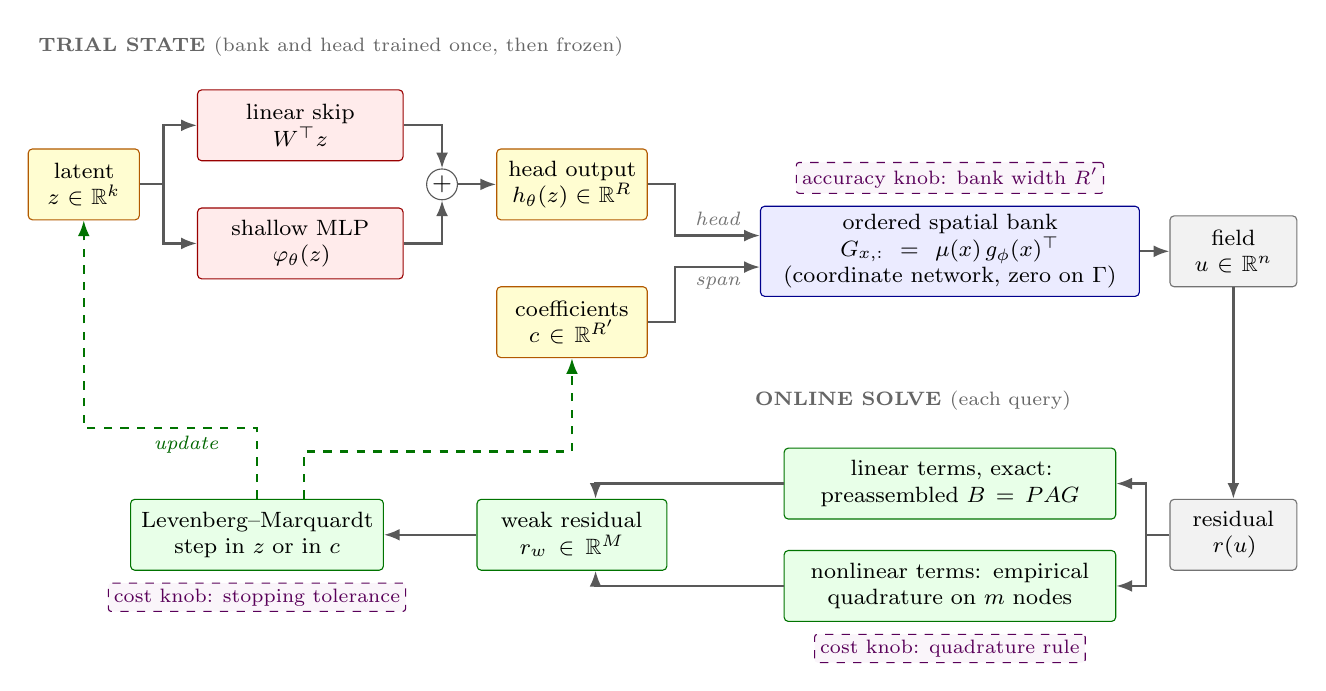
\begin{tikzpicture}[
  font=\footnotesize,
  box/.style={draw, rounded corners=1.5pt, minimum height=9mm, align=center,
              inner sep=3pt},
  dec/.style={box, fill=red!8, draw=red!60!black, text width=24mm},
  latent/.style={box, fill=yellow!18, draw=orange!70!black},
  bank/.style={box, fill=blue!8, draw=blue!55!black, text width=46mm},
  io/.style={box, fill=gray!10, draw=black!55},
  solve/.style={box, fill=green!9, draw=green!45!black},
  sum/.style={circle, draw=black!65, fill=white, inner sep=0.6pt, font=\small},
  knob/.style={draw=violet!70!black, dashed, rounded corners=1pt, fill=violet!4,
               font=\scriptsize, inner sep=2pt, text=violet!70!black},
  arr/.style={-{Latex[length=2mm]}, thick, draw=black!65},
  upd/.style={-{Latex[length=2mm]}, thick, dashed, draw=green!45!black},
  lbl/.style={font=\scriptsize\itshape, text=black!55},
  row/.style={font=\scriptsize\bfseries, text=black!60, anchor=west}
]
  % ===== TOP ROW: the trial state =====
  \node[row] at (-0.7,1.75) {TRIAL STATE \textmd{(bank and head trained once, then frozen)}};

  \node[latent, text width=12mm] (z) at (0,0) {latent\\$z\in\Real^{k}$};
  \node[dec] (skip) at (2.75,0.75) {linear skip\\$W\T z$};
  \node[dec] (mlp) at (2.75,-0.75) {shallow MLP\\$\varphi_\theta(z)$};
  \node[sum] (s1) at (4.55,0) {$+$};
  \node[latent, text width=17mm] (h) at (6.2,0) {head output\\$\head(z)\in\Real^{R}$};
  \node[latent, text width=17mm] (c) at (6.2,-1.75) {coefficients\\$c\in\Real^{R'}$};
  \node[bank] (G) at (11.0,-0.85) {ordered spatial bank\\$\bank_{x,:}=\bcmask(x)\,g_\phi(x)\T$\\(coordinate network, zero on $\Gamma$)};
  \node[io, text width=14mm] (u) at (14.6,-0.85) {field\\$u\in\Real^{n}$};

  \draw[arr] (z.east) -- ++(0.3,0) |- (skip.west);
  \draw[arr] (z.east) -- ++(0.3,0) |- (mlp.west);
  \draw[arr] (skip.east) -| (s1.north);
  \draw[arr] (mlp.east) -| (s1.south);
  \draw[arr] (s1) -- (h);
  \draw[arr] (h.east) -- ++(0.35,0) |- ([yshift=2mm]G.west)
       node[pos=0.75, above, lbl] {head};
  \draw[arr] (c.east) -- ++(0.35,0) |- ([yshift=-2mm]G.west)
       node[pos=0.75, below, lbl] {span};
  \draw[arr] (G) -- (u);

  \node[knob, above=1.5mm of G] {accuracy knob: bank width $R'$};

  % ===== BOTTOM ROW: online solve =====
  \node[row] at (8.4,-2.75) {ONLINE SOLVE \textmd{(each query)}};

  \node[io, text width=14mm] (res) at (14.6,-4.45) {residual\\$\rfull(u)$};
  \node[solve, text width=40mm] (lin) at (11.0,-3.8) {linear terms, exact:\\preassembled $B=\tests\Aop\bank$};
  \node[solve, text width=40mm] (eq) at (11.0,-5.1) {nonlinear terms: empirical\\quadrature on $m$ nodes};
  \node[solve, text width=22mm] (rw) at (6.2,-4.45) {weak residual\\$\rweak\in\Real^{M}$};
  \node[solve, text width=30mm] (lm) at (2.2,-4.45) {Levenberg--Marquardt\\step in $z$ or in $c$};

  \draw[arr] (u) -- (res);
  \draw[arr] (res.west) -- ++(-0.3,0) |- (lin.east);
  \draw[arr] (res.west) -- ++(-0.3,0) |- (eq.east);
  \draw[arr] (lin.west) -| ([xshift=3mm]rw.north);
  \draw[arr] (eq.west) -| ([xshift=3mm]rw.south);
  \draw[arr] (rw) -- (lm);
  \draw[upd] (lm.north) -- ++(0,0.9) -| (z.south);
  \draw[upd] ([xshift=6mm]lm.north) -- ++(0,0.6) -| (c.south);
  \node[lbl, text=green!40!black] at (1.3,-3.3) {update};

  \node[knob, below=1.5mm of eq] {cost knob: quadrature rule};
  \node[knob, below=1.5mm of lm] {cost knob: stopping tolerance};
\end{tikzpicture}
}
\caption{NM-ROM model and online solve. \textbf{Top, trained once and then
frozen:} the latent code $z$ passes through a linear skip and a shallow
SiLU network, and their sum gives the bank coefficients $\head(z)$. The
ordered coordinate-network bank, multiplied by a factor that vanishes on
the boundary $\Gamma$, turns coefficients into the field $u$ with the
Dirichlet data exact. A query uses either the head, $u=\bank\head(z)$, or
the span of the first $R'$ ordered columns, $u=\widehat{\bank}_{R'}c$.
\textbf{Bottom, solved at each query:} the residual of $u$ is tested
against $M$ fixed weak tests. Linear terms use the preassembled matrix $B$
and are exact; Burgers advection uses the empirical quadrature rule on $m$
nodes. A Levenberg--Marquardt step updates $z$ or $c$. Dashed tags mark
the deployment knobs: the bank width $R'$ sets the accuracy, and the
quadrature rule and the stopping tolerance set the cost.}
\label{fig:decoder}
\end{figure}

\paragraph{What is fixed and what is solved.}
\label{sec:method:tuning}\label{sec:method:layers}
Training fixes the bank, its ordering, the head and the tests for every
row of Table~\ref{tab:headline}. Each query solves $\latent$ or $c$.
Deployment chooses the mode and $R'$, the test count $M$, the quadrature
and the stopping rule, and leaves the weights fixed.

% =====================================================================
\section{Implementation}
\label{sec:impl}

\subsection{Matrix-free Projected Operators via JAX}

The matrix $B$ of \S\ref{sec:method:precomp} is built once per mesh, so
the online residual of a linear term is the product $Bc-b$. In the span
the Jacobian is the fixed matrix $BT_{:,1:R'}$. With the head the
remaining derivative is the Jacobian of the head, which forward-mode
automatic differentiation \citep{Bradbury2018JAX} supplies,
\begin{equation}
  \dhead\, v \;=\; \mathrm{JVP}(\head,\latent,v),
  \qquad
  J_\latent \;=\; B\,\dhead(\latent).
  \label{eq:jvp}
\end{equation}
Each accepted step solves the damped normal equation directly. A linear
PDE does not return to the grid, and the projected operator is not passed
to a Krylov method. Burgers advection reads the cached stencil on the
quadrature nodes; runs above $1024^2$ assemble its Jacobian analytically
(Appendix~\ref{app:method:burgers}). The ordered bank is stored in column
blocks at the tested widths, so a query at width $R'$ reads exactly $R'$
columns.

\subsection{Training Protocol}

Training is an auto-decoder on training data only, in two stages. The
coordinate network $g_\phi$ is fitted to the training states through
\eqref{eq:bank} and frozen, which fixes the bank. The head is then fitted
to the bank coefficients of those states, with one stored code per
training state. Last, the bank is ordered once by \eqref{eq:ordered}. This
step has no trainable weights and takes one QR and one SVD. Widths,
cohorts and offline costs are in Appendix~\ref{app:training-schedule}.

% =====================================================================
\section{Experimental Setup and Benchmark Problems}
\label{sec:setup}
\restoredisplays

\paragraph{Problems and references.}
In two dimensions we solve Poisson on the square, heat and viscous
Burgers, with an L-shaped Poisson domain as an ill-conditioned check. In
three dimensions we solve Poisson, heat and incompressible
Navier--Stokes on the periodic cube, whose initial velocity is the curl of
two localised vector potentials with random centre, separation, strength
and viscosity. Meshes and cohorts are in Table~\ref{tab:problems}, the
sampled families in Table~\ref{tab:spec} and the three-dimensional
configurations in Table~\ref{tab:config3d}.

\paragraph{Accuracy.}
We report the worst relative $L^2$ error over the stated cases and
requested times, in percent. Poisson uses the steady reference norm and
heat the current reference norm; Burgers and Navier--Stokes use the
initial-field norm over evolved times. Same-grid error measures the
reduction error against the converged discrete solution. Error against a
refined reference also includes discretisation error, and we never
interchange the two. Settings for a held-out cohort are fixed before its
cases are opened; all other cohorts are development cohorts.

\paragraph{Timing and speedup.}
Every accuracy--runtime pair comes from the same solver invocation, in
double precision, with GPU burn-in, synchronised timing and medians of
retained repetitions (protocol in Appendix~\ref{app:cg-current}). GPU
query time covers initialisation, the solve or rollout and the requested
device outputs. Training and compilation are offline costs. Speedup is
$S=T_{\mathrm{FOM}}/T_{\mathrm{method}}$ with both times from the same
allocation, and each table names the FOM and shows its error. Solves that
miss their stopping rule are reported as such and do not enter a
speedup.

\paragraph{Baselines.}
Poisson, including the L-shaped check, is compared with conjugate
gradients (CG), and heat with Crank--Nicolson stepping whose linear solve
is CG (CN--CG). Burgers is compared with Newton--BiCGStab. Navier--Stokes
is compared with the solver that generated its data, a Fourier
pseudo-spectral method with Crank--Nicolson diffusion and Adams--Bashforth
advection (CNAB2), which needs no linear solve. The named FOM of a row is
that solver at its fastest tested setting that is at least as accurate as
the accurate NM-ROM setting. Other nonlinear-manifold ROMs are compared in
Table~\ref{tab:nmrom-baselines}, and neural operators (FNO, U-Net,
DeepONet and Transolver) in Appendix~\ref{app:operators}.

\section{Numerical Experiments and Results}\label{sec:results}

Table~\ref{tab:headline} compares the NM-ROM with the named full-order
solvers at every problem and mesh. The subsections that follow look at
the bank-width knob behind the two settings of each row, and at which knob
to turn.

\subsection{Accuracy and Speed against Full-Order Solvers}
\label{sec:results:operators}\label{sec:exp:panel}

\begin{table}[t]
\centering
\caption{NM-ROM against the named full-order solver at every problem and
mesh. \textbf{Both NM-ROM columns of a row come from one frozen model}:
\emph{accurate} is the most accurate tested setting and \emph{fast} the
cheapest setting at least as accurate as the model's earlier default
(Table~\ref{tab:headline-times}); no network is retrained between them.
Error is the worst relative $L^2$ error over the cases (\%). Speedup is the
FOM's median time divided by the NM-ROM's in the same GPU allocation,
\textbf{bold} where the NM-ROM is faster. The FOM is the named solver at
its fastest tested setting at least as accurate as the accurate setting,
and both speedups of a row divide that one time. Navier--Stokes is
compared with CNAB2, the Fourier pseudo-spectral solver that generated
its data, which needs no linear solve; its fast setting is the cheapest
bank width below 5\,\% error. Rows marked $^{o}$ use the ordered bank;
the others still use the earlier correction settings until their reruns
finish. Marker definitions are in Appendix~\ref{app:cg-current}. Dashes
mark settings not measured.}
\label{tab:headline}
\resizebox{\linewidth}{!}{% GENERATED by paper/gen_headline.py from hash-pinned snapshots -- do not edit.
\small\setlength{\tabcolsep}{4pt}
\begin{tabular}{@{}llrrrrrl@{}}
\toprule
 & & \multicolumn{2}{c}{NM-ROM accurate} & \multicolumn{2}{c}{NM-ROM fast} & \multicolumn{2}{c}{Full-order model (FOM)} \\
\cmidrule(lr){3-4}\cmidrule(lr){5-6}\cmidrule(l){7-8}
Problem & Mesh & Err.\ (\%) & Speedup & Err.\ (\%) & Speedup & Err.\ (\%) & Solver \\
\midrule
\multicolumn{8}{@{}l}{\emph{Two-dimensional}} \\
Poisson$^{o}$ & $256^2$$^{p}$ & 0.75 & \textbf{13.4$\times$} & 2.31 & \textbf{17.5$\times$} & 0.55 & CG, rtol $3{\times}10^{-2}$ \\
 & $1024^2$$^{p}$ & 0.74 & \textbf{27.9$\times$} & 2.31 & \textbf{68.5$\times$} & 0.22 & CG, rtol $3{\times}10^{-2}$ \\
 & $2048^2$ & 0.74 & \textbf{54.1$\times$} & 2.31 & \textbf{174$\times$} & 0.61 & CG, rtol $10^{-1}$ \\
 & $4096^2$ & 0.74 & \textbf{106$\times$} & 2.31 & \textbf{358$\times$} & 0.45 & CG, rtol $10^{-1}$ \\
Poisson, L-shape$^{c}$ & $256^2$ & 2.13 & \textbf{3.84$\times$} & 3.86 & \textbf{4.04$\times$} & 0.64 & CG, rtol $10^{-2}$ \\
 & $512^2$ & 2.12 & \textbf{6.07$\times$} & 3.85 & \textbf{6.18$\times$} & 0.38 & CG, rtol $10^{-2}$ \\
 & $1024^2$ & 2.20 & \textbf{8.38$\times$} & 3.85 & \textbf{8.59$\times$} & 1.05 & CG, rtol $3{\times}10^{-2}$ \\
 & $2048^2$ & 2.20 & \textbf{17.0$\times$} & 3.85 & \textbf{17.1$\times$} & 0.76 & CG, rtol $3{\times}10^{-2}$ \\
Heat$^{t}$$^{f}$$^{a}$ & $1024^2$ & 0.49 & \textbf{13.9$\times$} & 1.36 & \textbf{13.0$\times$} & 0.18 & CN--CG, $\Delta t{=}0.05$, rtol $10^{-3}$ \\
 & $2048^2$ & 0.49 & \textbf{60.0$\times$} & 1.36 & \textbf{57.0$\times$} & 0.18 & CN--CG, $\Delta t{=}0.05$, rtol $10^{-3}$ \\
 & $4096^2$ & 0.49 & \textbf{103$\times$} & 1.36 & \textbf{101$\times$} & 0.47 & CN--CG, $\Delta t{=}0.05$, rtol $10^{-2}$ \\
Burgers$^{e}$ & $256^2$ & 0.51$^{s}$ & 0.043$\times$ & 1.89 & 0.79$\times$ & 0.049 & Newton--BiCGStab, tol $10^{-3}$ \\
 & $512^2$ & 0.55$^{x}$ & 0.068$\times$ & 2.14 & \textbf{1.31$\times$} & 0.052 & Newton--BiCGStab, tol $10^{-3}$ \\
 & $1024^2$ & 0.59$^{d}$ & 0.0037$\times$ & 2.29 & \textbf{2.02$\times$} & 0.034 & Newton--BiCGStab, tol $10^{-4}$ \\
 & $2048^2$ & 0.87$^{\ell}$ & 0.99$\times$ & 2.37 & \textbf{4.16$\times$} & 0.049 & Newton--BiCGStab, tol $3{\times}10^{-3}$ \\
 & $4096^2$ & 0.60$^{w}$ & \textbf{4.87$\times$} & 2.41 & \textbf{10.10$\times$} & 0.050 & Newton--BiCGStab, tol $3{\times}10^{-3}$ \\
\midrule
\multicolumn{8}{@{}l}{\emph{Three-dimensional}} \\
Poisson$^{f}$ & $32^3$ & 0.26 & 0.94$\times$ & 1.40 & 0.99$\times$ & 0.16 & CG, rtol $10^{-2}$ \\
 & $64^3$ & 0.26 & \textbf{1.33$\times$} & 1.39 & \textbf{1.38$\times$} & 0.11 & CG, rtol $10^{-2}$ \\
Poisson (dev. sources) & $128^3$ & 0.16 & \textbf{6.75$\times$} & 0.55 & \textbf{6.98$\times$} & 0.075 & CG, rtol $10^{-2}$ \\
 & $256^3$ & 0.16 & \textbf{23.2$\times$} & 0.55 & \textbf{23.7$\times$} & 0.049 & CG, rtol $10^{-2}$ \\
Heat$^{t}$$^{f}$$^{a}$ & $32^3$ & 0.11 & 0.62$\times$ & 2.00 & 0.57$\times$ & 0.078 & CN--CG, $\Delta t{=}0.025$, rtol $10^{-4}$ \\
 & $64^3$ & 0.11 & 0.94$\times$ & 2.00 & 0.85$\times$ & 0.081 & CN--CG, $\Delta t{=}0.025$, rtol $10^{-4}$ \\
 & $128^3$ & 0.11 & \textbf{2.22$\times$} & 2.00 & \textbf{2.10$\times$} & 0.082 & CN--CG, $\Delta t{=}0.025$, rtol $10^{-4}$ \\
Navier--Stokes$^{e}$$^{o}$ & $32^3$ & 0.15 & \textbf{1.09$\times$} & 2.96 & \textbf{1.87$\times$} & 0.094 & CNAB2 (spectral), 50 steps \\
 & $64^3$ & 0.15 & \textbf{2.89$\times$} & 2.96 & \textbf{5.09$\times$} & 0.093 & CNAB2 (spectral), 50 steps \\
 & $96^3$ & 0.15 & \textbf{6.67$\times$} & 2.96 & \textbf{11.6$\times$} & 0.063 & CNAB2 (spectral), 60 steps \\
\bottomrule
\end{tabular}
}
\end{table}

\paragraph{Linear problems.}
On Poisson both settings of a row are solves in the span of the ordered
bank. At $4096^2$ the accurate width $R'=512$ reaches
$\nBwPoisAccErr\,\%$ at $\nBwPoisAccS\times$ the speed of CG, and the fast
width $R'=128$ reaches $\nBwPoisFastErr\,\%$ at $\nBwPoisFastS\times$. The
head is less accurate here ($\nBwPoisHeadErr\,\%$): on a linear problem
the best solve in the bank is the linear one, and it is also the cheapest.
The speedup grows with the mesh because the reduced query does not visit
the grid until it returns the field. On the L-shaped check the accurate
setting is $\nHeadLshapeAccS\times$ faster at $\nHeadLshapeAccErr\,\%$. A
wide heat bank, evaluated once on a sealed held-out cohort at every mesh,
reaches $\nHeatWideAccErr\,\%$ over all times and is
$\nHeatWideBatchedAccS\times$ faster than CN--CG at $4096^2$. In three
dimensions the held-out Poisson cohort gives
$\nHeadPoissonThreeAccErr\,\%$ at $\nHeadPoissonThreeAccS\times$. The
three-dimensional heat bank, evaluated once on a sealed cohort of
\nHeatNewCases{} cases, meets the 1\,\% all-times target at every mesh
(accurate $\nHeatNewAccErr\,\%$) and overtakes CN--CG at $128^3$
($\nHeatNewBfAccS\times$). \todo{L-shape, heat and 3D Poisson rows: bank-width reruns running; numbers above are the current checkpoint's.}

\paragraph{Burgers.}
\todo{Burgers rows still come from the earlier correction-direction solve; the bank-width rerun is running and replaces this paragraph.}
The reduced solve costs about the same at every mesh, so the fast setting
overtakes Newton--BiCGStab by $1024^2$ ($\nHeadBurgersFastS\times$ faster
at $\nHeadBurgersFastErr\,\%$ error). At $4096^2$ the accurate setting
chosen on six development cases reaches $\nBurgDevAccErrFortyNinetySix\,\%$
and is $\nBurgDevAccSFortyNinetySix\times$ faster than the fastest Newton
setting at least as accurate. On 64 held-out cases the same setting gives
$\nBurgHoldAccErrFortyNinetySix\,\%$ at
$\nBurgHoldAccSFortyNinetySix\times$. The quadrature rule of those rows
passes five held-out draws and fails the confirmation draw, so it is
validated but not confirmed (Appendix~\ref{app:cg-current}).

\paragraph{Navier--Stokes.}
Here the head earns its place. At $96^3$ the head with $k=\nNsHeadK$
reaches $\nNsHeadErr\,\%$ and is $\nNsHeadS\times$ faster than CNAB2 at
matched accuracy. The span of the same bank is
$\nNsHeadVsSpan\times$ less accurate at the same number of unknowns, and
even the full rank-$\nNsBankR$ span reaches only $\nNsSpanWideErr\,\%$.
The moving vortices lie on a low-dimensional curved manifold that the
head follows and a small linear span does not. The error stays flat from
$32^3$ to $96^3$ while the speedup rises from $\nNsSmallS\times$ to
$\nNsHeadS\times$. On \nNsHoldCases{} held-out cases the frozen settings
give $\nNsHoldHeadErr\,\%$ at $\nNsHoldHeadS\times$.

\paragraph{Resolution.}
In every series of Table~\ref{tab:headline} the NM-ROM query time grows
more slowly with the mesh than the FOM's, so the speedup rises with
resolution while the error stays near its coarse-mesh value. The selected
FOM setting may change with the mesh, since it must match the accurate
setting at each one.

\begin{table}[t]
\centering
\caption{Other nonlinear-manifold ROMs on the shared Burgers 2D family at
$256^2$ and $512^2$: worst and median evolved same-grid error over 32
validation cases (never used for any choice) and compiled-query memory,
one allocation. Latent dimension is matched for the baselines and our fast
setting. The shallow masked-autoencoder NM-LSPG of
\citet{KimChoi2022NMROM} passed its reproduction gate on the third of
three pre-registered attempts; its hyper-reduction was not reproduced, and
its published encoder width does not fit our devices, so at $512^2$ its
width-capped encoder is limited by training time
(Table~\ref{tab:nmrom-baselines-appx}, which also states the data-matched
row and the residual path). Every row here, ours included, uses a dense
residual, so no times are given.}
\label{tab:nmrom-baselines}
\resizebox{\linewidth}{!}{% GENERATED by paper/gen_headline.py -- slot for the nmrom-baselines lane; no value is read until an audited summary is supplied.
\small
\begin{tabular}{@{}llrr@{}}
\toprule
Problem, mesh & Method & Err.\ (\%) & Speedup vs.\ FOM \\
\midrule
--- & This work (accurate / fast) & --- & --- \\
--- & Convolutional-autoencoder NM-ROM & --- & --- \\
--- & Shallow-masked-autoencoder NM-ROM & --- & --- \\
\bottomrule
\end{tabular}
}
\end{table}

On 32 validation Burgers cases at $256^2$ and $512^2$
(Table~\ref{tab:nmrom-baselines}) our fast setting, at matched latent
dimension, reaches worst errors of $\nBaseOursFastWorst\,\%$, against
$\nBaseKimRange\,\%$ for the reproduced shallow masked-autoencoder NM-ROM
and $\nBasePodRange\,\%$ for POD-LSPG. Our accurate setting reaches
$\nBaseOursAccWorst\,\%$. \todo{add the quadratic-manifold row (QM16) and the bank-width rows from the high-resolution comparison.}

\begin{table}[t]
\centering
\caption{Bank-width tunability at the finest mesh. Each block is one frozen
model, and within a cohort every speedup divides the median time of
\emph{one} full-order setting (the \emph{FOM} row, the fastest at least
as accurate as the block's most accurate setting, in the same allocation)
by the setting's time (ms). Error is the worst same-grid relative $L^2$ error (\%), over
evolved times for Navier--Stokes, Burgers and heat. Held-out cases were
never used for selection and share the development settings.
\todo{Burgers and heat blocks still show the earlier correction ladder;
their bank-width reruns are running.}}
\label{tab:tunability}
% GENERATED by paper/gen_tunability_table.py from tables/headline-provenance.json -- do not edit.
\small\setlength{\tabcolsep}{4pt}
\begin{tabular}{@{}lrrrrrr@{}}
\toprule
 & \multicolumn{3}{c}{Development cohort} & \multicolumn{3}{c}{Held-out cohort} \\
\cmidrule(lr){2-4}\cmidrule(l){5-7}
Setting & Err.\ (\%) & ms & Speedup & Err.\ (\%) & ms & Speedup \\
\midrule
\multicolumn{7}{@{}l}{\emph{Poisson 2D, ordered bank, $4096^2$ (12 development sources)}} \\
Head, $k{=}32$, $R'{=}512$ & 3.15 & 43.4 & 103$\times$ & --- & --- & --- \\
Bank span, $R'{=}512$ & 0.74 & 42.4 & 106$\times$ & --- & --- & --- \\
Bank span, $R'{=}384$ & 0.77 & 32.5 & 138$\times$ & --- & --- & --- \\
Bank span, $R'{=}256$ & 0.94 & 22.6 & 199$\times$ & --- & --- & --- \\
Bank span, $R'{=}128$ & 2.31 & 12.5 & 358$\times$ & --- & --- & --- \\
Bank span, $R'{=}64$ & 5.33 & 7.1 & 631$\times$ & --- & --- & --- \\
Bank span, $R'{=}32$ & 9.17 & 4.4 & 1022$\times$ & --- & --- & --- \\
\emph{FOM:} CG, rtol $10^{-1}$ & 0.45 & 4490 & 1$\times$ & --- & --- & --- \\
\midrule
\multicolumn{7}{@{}l}{\emph{Navier--Stokes 3D, co-moving frame, ordered bank, $96^3$ (16 development / 32 held-out cases)}} \\
Head, $k{=}8$ & 0.15 & 16.0 & 6.67$\times$ & 0.21 & 15.8 & 7.79$\times$ \\
Bank span, $R'{=}64$ & 0.62 & 15.4 & 6.92$\times$ & 1.12 & 15.3 & 8.05$\times$ \\
Bank span, $R'{=}48$ & 1.00 & 12.9 & 8.27$\times$ & 1.26 & 12.6 & 9.76$\times$ \\
Bank span, $R'{=}32$ & 1.26 & 11.6 & 9.14$\times$ & 1.46 & 11.5 & 10.7$\times$ \\
Bank span, $R'{=}16$ & 2.96 & 9.2 & 11.6$\times$ & 3.24 & 9.2 & 13.4$\times$ \\
Bank span, $R'{=}8$ & 5.55 & 8.2 & 13.0$\times$ & 6.91 & 8.1 & 15.2$\times$ \\
\emph{FOM:} CNAB2 (spectral), 60 / 70 steps & 0.063 & 106 & 1$\times$ & 0.056 & 123 & 1$\times$ \\
\midrule
\multicolumn{7}{@{}l}{\emph{Burgers 2D, correction rank (6 development / 64 held-out cases)}} \\
$q=0$, $M=64$ & 2.41 & 40.7 & 12.9$\times$ & 9.03 & 40.6 & 13.2$\times$ \\
$q=128$, $M=576$ & 1.09 & 77.4 & 6.77$\times$ & 2.43 & 74.6 & 7.21$\times$ \\
$q=256$, $M=544$ & 0.88 & 112 & 4.67$\times$ & 2.93 & 105 & 5.11$\times$ \\
$q=256$, $M=1088$ & 0.60 & 127 & 4.12$\times$ & 1.33 & 113 & 4.77$\times$ \\
$q=256$, $M=1088$, looser tol.$^{\star}$ & 0.60 & 108 & 4.87$\times$ & 1.33 & 100 & 5.38$\times$ \\
$q=256$, $M=2176$$^{\dagger}$ & 0.46 & 132 & 3.96$\times$ & 1.13 & 126 & 4.25$\times$ \\
\emph{FOM:} Newton--BiCGStab, tol.\ $3{\times}10^{-3}$ & 0.050 & 524 & 1$\times$ & 0.14 & 537 & 1$\times$ \\
\midrule
\multicolumn{7}{@{}l}{\emph{Heat 2D, wide bank, correction rank (16 sealed held-out cases)}} \\
$q=0$ & --- & --- & --- & 0.84 & 32.2 & 146$\times$ \\
$q=32$ & --- & --- & --- & 0.22 & 31.7 & 149$\times$ \\
$q=96$ & --- & --- & --- & 0.082 & 24.4 & 193$\times$ \\
\emph{FOM:} CN--CG, $\Delta t=0.025$, rtol $10^{-6}$ & --- & --- & --- & 0.045 & 4713 & 1$\times$ \\
\bottomrule
\end{tabular}

\end{table}

\paragraph{Settings.}\label{sec:results:best}
Table~\ref{tab:tunability} shows the whole ladder behind the two settings
of a row. On Poisson at $4096^2$, narrowing the bank from $R'=512$ to $32$
raises the error $\nBwPoisErrSpan\times$, from $\nBwPoisAccErr$ to
$\nBwPoisNarrowErr\,\%$, and lowers the query time $\nBwPoisCostSpan\times$,
so the same model moves from $\nBwPoisAccS\times$ to $\nBwPoisNarrowS\times$
the speed of CG. On Navier--Stokes the span ladder runs from
$\nNsSpanWideErr\,\%$ at $R'=64$ to $\nNsSpanNarrowErr\,\%$ at $R'=8$, at
$\nNsSpanCostSpan\times$ lower cost, and the head sits above it in
accuracy. Moving along a ladder never requires retraining, only a new
deployment argument. This is what we mean by deployment-time tunability.

\subsection{Which Knob to Turn}\label{sec:results:tunability}

We sort the knobs of the framework into three groups
(Table~\ref{tab:knobs-main}). The first is the \emph{deployment-time
accuracy} knob, the bank width $R'$ together with the choice between head
and span, which changes what the trained model can represent. The second
holds the \emph{deployment-time cost} knobs, the quadrature rule and the
stopping tolerance, which change how the residual is evaluated and when
the solve stops, at little change in error. The third holds
\emph{engineering} choices in the solver path, which do not change the
answer but set how long it takes. The iteration cap is a safeguard, not a
knob, since a truncated solve fails.

\begin{table}[t]
\centering
\caption{Which knob to turn, measured from frozen models. Bank width:
Table~\ref{tab:tunability}. EQ: dense time over EQ time for Burgers in one
allocation per mesh. Tolerance and cap: 32 validation Burgers cases
(Table~\ref{tab:knobs}), stopping tolerance $10^{-8}\!\to\!10^{-3}$ and
iteration cap 2. The engineering row leaves the iterates unchanged.
$^{\ast}$\,Jobs \provPanelJob{} and \provPanelTenTwentyFourJob{}.}
\label{tab:knobs-main}
\resizebox{\linewidth}{!}{%
\begin{tabular}{@{}llll@{}}
\toprule
Knob & Turn it to & Effect on error & Effect on cost \\
\midrule
\multicolumn{4}{@{}l}{\emph{Deployment time, accuracy (no retraining):}} \\
Bank width $R'$, Poisson $4096^2$ & $512\to32$ & $\nBwPoisErrSpan\times$ higher & $\nBwPoisCostSpan\times$ lower \\
Bank width $R'$, Navier--Stokes $96^3$ & $64\to8$ & $\nNsSpanWideErr\to\nNsSpanNarrowErr\,\%$ & $\nNsSpanCostSpan\times$ lower \\
Head instead of span, Navier--Stokes $96^3$ & $R'=k=\nNsHeadK$ & $\nNsHeadVsSpan\times$ lower & higher (Table~\ref{tab:tunability}) \\
\multicolumn{4}{@{}l}{\emph{Deployment time, cost (no retraining):}} \\
Empirical quadrature & dense $\to$ stored rule & Table~\ref{tab:figure1-table} & $\nPanelEqSpeedupZero\times$ lower at $256^2$, $\nPanelTenTwentyFourEqSpeedupZero\times$ at $1024^2$$^{\ast}$ \\
Stopping tolerance & looser & $\nTuneTolErrConverged\to\nTuneTolErrLoose\,\%$ & $\nTuneTolSavingPct\,\%$ lower \\
\multicolumn{4}{@{}l}{\emph{Engineering (same answer):}} \\
Solver path & before $\to$ after & unchanged & \gen{$1024^2$ gain, job 4187625} lower \\
\multicolumn{4}{@{}l}{\emph{Safeguard:}} \\
Iteration cap & 2 iterations & fails ($\nTuneCapTwoErr\,\%$) & --- \\
\bottomrule
\end{tabular}}
\end{table}

The first group is what makes the NM-ROM tunable in a way a trained
neural operator is not: the same frozen model is reused, and only a
deployment argument changes. Which end to use depends on the problem. On
the linear problems the span wins at every width, so the knob is $R'$
alone. On Navier--Stokes the head is the accurate end and the span ladder
the fast end, and the head costs about twice the time of the span at the
same number of unknowns, because each step also evaluates the network and
its Jacobian.

The second group lowers the cost of a chosen accuracy. Empirical
quadrature removes the mesh from the Burgers residual
(\S\ref{sec:method:precomp}), and a looser stopping tolerance saves time
at the same error. Neither changes the trial space, so neither can buy
accuracy.

The engineering group contributes most of the Burgers speedup at fine
meshes. The solver path of the current rows (Cholesky factorisation of
the damped normal equation, a clipped step, damping carried between
steps, a quadratic predictor and an analytic Jacobian;
Appendix~\ref{app:method:burgers}) reaches the same error as the path it
replaced \gen{$1024^2$ gain}$\times$ faster in one allocation. Each change
is checked to reproduce the replaced path's iterates and iteration
counts.

\paragraph{Limitations.}\label{sec:limitations}
\label{sec:results:head}\label{sec:results:collapse}\label{sec:exp:eq}
(i) Except for Navier--Stokes, speedups are against named iterative
full-order solvers at the stated tolerances. Fast direct and spectral
solvers exist for the square and the cube and would be faster than CG
there. The named FOM is more accurate than the NM-ROM in every row.
(ii) The Navier--Stokes bank is a POD basis in a moving frame, not a
coordinate network, and the family has moderate Reynolds numbers; we make
no claim about turbulent flow.
(iii) On Poisson the errors lie near the bank floor
($\nHiresFloorSquare\,\%$ square, $\nHiresFloorCube\,\%$ cube), so a wider
or better bank, not the solver, limits accuracy. The L-shape
($\nHiresLshapeAccErr\,\%$ against a floor of $\nHiresLshapeFloor\,\%$) is
limited by the head.
(iv) Quadrature validation covers finitely many reached states and is not
a global certificate. The $4096^2$ Burgers rule is not confirmed on
independent re-draws, and no rule is used in three dimensions. Reduced
solves can converge to a wrong branch, and lower same-grid error does not
remove discretisation error.
(v) Unmarked cohorts are small development cohorts; exceptions are marked
held-out. Timings report medians without dispersion.

\section{Conclusion and Future Work}\label{sec:conclusion}

We built an NM-ROM whose distinguishing property is a deployment-time
accuracy/speed tradeoff from a single trained model: at inference, the
width of the ordered bank, the choice between the head and the span, the
quadrature rule and the stopping tolerance trade accuracy for speed. This
is the lever neural operators do not expose, since each trained FNO or
DeepONet delivers one fixed operating point. Mechanically, the decoder is
a learned manifold built from a coordinate-network bank and a nonlinear
head; the PDE itself is enforced by least-squares Petrov--Galerkin
projection of the discrete residual onto that manifold; Dirichlet
boundary conditions are enforced exactly by the bank; linear terms are
preassembled exactly and empirical quadrature removes the mesh from the
nonlinear term; and the whole pipeline is matrix-free in JAX.

Three pieces had to come together to make this work. First, a
coordinate-network bank, which is evaluated at one node without the
others and serves every mesh of a series from one trained network.
Second, a one-time ordering of that bank, which turns one trained model
into a nested family of trial spaces chosen at the query. Third, a head
with a linear skip, which gives the latent solve a usable direction from a
stored code and supplies the accurate end where a linear span is not
enough, as on Navier--Stokes.

The model keeps its accuracy as the mesh is refined, so its speedup over
the named solvers grows with resolution. At $4096^2$ it reaches
$\nBwPoisAccErr\,\%$ on Poisson at $\nBwPoisAccS\times$ the speed of CG,
and on three-dimensional Navier--Stokes at $96^3$ the head reaches
$\nNsHeadErr\,\%$ at $\nNsHeadS\times$ the speed of a spectral solver,
$\nNsHeadVsSpan\times$ more accurate than a linear span of the same size.
The named solvers remain more accurate. A natural next step is a
coordinate-network bank for moving-frame flows, quadrature in three
dimensions, and advection-dominated three-dimensional problems.

\section*{Reproducibility statement}\label{sec:repro}
Every table and prose number is generated from hash-pinned run records
identifying source, checkpoint, settings, cohort, allocation and audit
(Appendix~\ref{app:provenance}); failed settings are kept.

\section*{AI use statement}
Language-model assistants supported method and experiment development,
implementation, analysis, auditing and drafting. Recorded solver runs
produced the numbers and the generators reproduce them. The authors are
responsible for the methods, results and text.

\enlargethispage{\baselineskip}
\bibliographystyle{plainnat}
\begin{thebibliography}{99}

\bibitem[Barnett and Farhat(2022)]{BarnettFarhat2022}
J.~Barnett and C.~Farhat.
\newblock Quadratic approximation manifold for mitigating the
Kolmogorov barrier in nonlinear projection-based model order reduction.
\newblock \emph{Journal of Computational Physics}, 464:111348, 2022.
\bibitem[Benner et~al.(2015)]{BennerGugercinWillcox2015}
P.~Benner, S.~Gugercin, and K.~Willcox.
\newblock A survey of projection-based model reduction methods for
parametric dynamical systems.
\newblock \emph{SIAM Review}, 57(4):483--531, 2015.

\bibitem[Berkooz et~al.(1993)]{Berkooz1993}
G.~Berkooz, P.~Holmes, and J.~L. Lumley.
\newblock The proper orthogonal decomposition in the analysis of
turbulent flows.
\newblock \emph{Annual Review of Fluid Mechanics}, 25(1):539--575, 1993.

\bibitem[Berrone et~al.(2022)]{BerroneBC2022}
S.~Berrone, C.~Canuto, M.~Pintore, and N.~Sukumar.
\newblock Enforcing Dirichlet boundary conditions in physics-informed
neural networks and variational physics-informed neural networks.
\newblock \emph{arXiv preprint arXiv:2210.14795}, 2022.

\bibitem[Boull\'e and Townsend(2024)]{BoulleTownsend2024}
N.~Boull\'e and A.~Townsend.
\newblock A mathematical guide to operator learning.
\newblock In \emph{Handbook of Numerical Analysis}, volume~25, pages
83--125. Elsevier, 2024.

\bibitem[Bradbury et~al.(2018)]{Bradbury2018JAX}
J.~Bradbury, R.~Frostig, P.~Hawkins, M.~J. Johnson, C.~Leary,
D.~Maclaurin, G.~Necula, A.~Paszke, J.~VanderPlas, S.~Wanderman-Milne,
and Q.~Zhang.
\newblock JAX: composable transformations of Python+NumPy programs, 2018.

\bibitem[Brecht et~al.(2023)]{BrechtHardConstraints2023}
R.~Brecht, R.~O. Popovych, A.~Bihlo, and Y.~Popovych.
\newblock Improving physics-informed DeepONets with hard constraints.
\newblock \emph{arXiv preprint arXiv:2309.07899}, 2023.

\bibitem[Cai et~al.(2020)]{Cai2020OnceForAll}
H.~Cai, C.~Gan, T.~Wang, Z.~Zhang, and S.~Han.
\newblock Once-for-All: Train one network and specialize it for
efficient deployment.
\newblock In \emph{International Conference on Learning Representations},
2020.

\bibitem[Cao(2021)]{Cao2021GalerkinTransformer}
S.~Cao.
\newblock Choose a Transformer: Fourier or Galerkin.
\newblock In \emph{Advances in Neural Information Processing Systems},
2021.

\bibitem[Carlberg et~al.(2011)]{Carlberg2011LSPG}
K.~Carlberg, C.~Bou-Mosleh, and C.~Farhat.
\newblock Efficient non-linear model reduction via a least-squares
Petrov--Galerkin projection and compressive tensor approximations.
\newblock \emph{International Journal for Numerical Methods in
Engineering}, 86(2):155--181, 2011.

\bibitem[Chaturantabut and Sorensen(2010)]{ChaturantabutSorensen2010}
S.~Chaturantabut and D.~C. Sorensen.
\newblock Nonlinear model reduction via discrete empirical
interpolation.
\newblock \emph{SIAM Journal on Scientific Computing}, 32(5):2737--2764,
2010.

\bibitem[Chen et~al.(2024)]{Chen2024UnsupervisedNO}
W.~Chen, J.~Song, P.~Ren, S.~Subramanian, D.~Morozov, and M.~W.
Mahoney.
\newblock Data-efficient operator learning via unsupervised pretraining
and in-context learning.
\newblock In \emph{Advances in Neural Information Processing Systems},
2024.

\bibitem[Cohen and DeVore(2015)]{CohenDeVore2015}
A.~Cohen and R.~DeVore.
\newblock Approximation of high-dimensional parametric PDEs.
\newblock \emph{Acta Numerica}, 24:1--159, 2015.

\bibitem[Diaz et~al.(2024)]{Diaz2024DomainDecompNMROM}
A.~N. Diaz, Y.~Choi, and M.~Heinkenschloss.
\newblock A fast and accurate domain-decomposition nonlinear manifold
reduced order model.
\newblock \emph{Computer Methods in Applied Mechanics and Engineering},
425:116943, 2024.

\bibitem[Dosovitskiy et~al.(2021)]{Dosovitskiy2021ViT}
A.~Dosovitskiy, L.~Beyer, A.~Kolesnikov, D.~Weissenborn, X.~Zhai,
T.~Unterthiner, M.~Dehghani, M.~Minderer, G.~Heigold, S.~Gelly,
J.~Uszkoreit, and N.~Houlsby.
\newblock An image is worth 16x16 words: Transformers for image
recognition at scale.
\newblock In \emph{International Conference on Learning Representations},
2021.

\bibitem[Eshaghi et~al.(2025)]{EshaghiNOWS2025}
M.~S. Eshaghi, C.~Anitescu, N.~Valizadeh, Y.~Wang, X.~Zhuang, and
T.~Rabczuk.
\newblock NOWS: Neural operator warm starts for accelerating iterative
solvers.
\newblock \emph{arXiv preprint arXiv:2511.02481}, 2025.

\bibitem[Farhat et~al.(2014)]{FarhatECSW2014}
C.~Farhat, P.~Avery, T.~Chapman, and J.~Cortial.
\newblock Dimensional reduction of nonlinear finite element dynamic
models with finite rotations and energy-based mesh sampling and
weighting for computational efficiency.
\newblock \emph{International Journal for Numerical Methods in
Engineering}, 98(9):625--662, 2014.

\bibitem[Fresca and Manzoni(2022)]{FrescaManzoni2022PODDLROM}
S.~Fresca and A.~Manzoni.
\newblock POD-DL-ROM: Enhancing deep learning-based reduced order
models for nonlinear parametrized PDEs by proper orthogonal decomposition.
\newblock \emph{Computer Methods in Applied Mechanics and Engineering},
388:114181, 2022.

\bibitem[Geelen et~al.(2022)]{GeelenWrightWillcox2022}
R.~Geelen, S.~Wright, and K.~Willcox.
\newblock Operator inference for non-intrusive model reduction with
quadratic manifolds.
\newblock \emph{Computer Methods in Applied Mechanics and Engineering},
403:115717, 2022.

\bibitem[Greif and Urban(2019)]{GreifUrban2019}
C.~Greif and K.~Urban.
\newblock Decay of the Kolmogorov $N$-width for wave problems.
\newblock \emph{Applied Mathematics Letters}, 96:216--222, 2019.

\bibitem[Griewank and Walther(2008)]{GriewankWalther2008}
A.~Griewank and A.~Walther.
\newblock \emph{Evaluating Derivatives: Principles and Techniques of
Algorithmic Differentiation}.
\newblock SIAM, Philadelphia, 2nd edition, 2008.

\bibitem[Hao et~al.(2023)]{HaoGNOT2023}
Z.~Hao, Z.~Wang, H.~Su, C.~Ying, Y.~Dong, S.~Liu, Z.~Cheng, J.~Song,
and J.~Zhu.
\newblock GNOT: A general neural operator transformer for operator
learning.
\newblock In \emph{International Conference on Machine Learning}, 2023.

\bibitem[Hao et~al.(2024)]{HaoDPOT2024}
Z.~Hao, C.~Su, S.~Liu, J.~Berner, C.~Ying, H.~Su, A.~Anandkumar,
J.~Song, and J.~Zhu.
\newblock DPOT: Auto-regressive denoising operator transformer for
large-scale PDE pre-training.
\newblock In \emph{International Conference on Machine Learning}, 2024.

\bibitem[Herde et~al.(2024)]{HerdePoseidon2024}
M.~Herde, B.~Raonic, T.~Rohner, R.~K\"appeli, R.~Molinaro,
E.~de~Bezenac, and S.~Mishra.
\newblock Poseidon: Efficient foundation models for PDEs.
\newblock In \emph{Advances in Neural Information Processing Systems},
2024.

\bibitem[Hern\'andez et~al.(2017)]{Hernandez2017EQ}
J.~A. Hern\'andez, M.~A. Caicedo, and A.~Ferrer.
\newblock Dimensional hyper-reduction of nonlinear finite element
models via empirical cubature.
\newblock \emph{Computer Methods in Applied Mechanics and Engineering},
313:687--722, 2017.

\bibitem[Hestenes and Stiefel(1952)]{HestenesStiefel1952CG}
M.~R. Hestenes and E.~Stiefel.
\newblock Methods of conjugate gradients for solving linear systems.
\newblock \emph{Journal of Research of the National Bureau of Standards},
49(6):409--436, 1952.

\bibitem[Hesthaven et~al.(2016)]{HesthavenRozzaStamm2016}
J.~S. Hesthaven, G.~Rozza, and B.~Stamm.
\newblock \emph{Certified Reduced Basis Methods for Parametrized
Partial Differential Equations}.
\newblock SpringerBriefs in Mathematics. Springer, 2016.

\bibitem[Hirsch et~al.(2024)]{HirschPichiHesthavenNEIM2024}
M.~Hirsch, F.~Pichi, and J.~S. Hesthaven.
\newblock Neural empirical interpolation method for nonlinear model
reduction.
\newblock \emph{arXiv preprint arXiv:2406.03562}, 2024.

\bibitem[Holzschuh et~al.(2025)]{HolzschuhPDETransformer2025}
B.~Holzschuh, Q.~Liu, G.~Kohl, and N.~Thuerey.
\newblock PDE-Transformer: Efficient and versatile transformers for
physics simulations.
\newblock In \emph{International Conference on Machine Learning}, 2025.

\bibitem[Hu et~al.(2025)]{HuLinearNO2025}
W.~Hu, S.~Liu, P.~Qiao, Z.~Sun, and Y.~Dou.
\newblock Transolver is a linear transformer: Revisiting
physics-attention through the lens of linear attention.
\newblock \emph{arXiv preprint arXiv:2511.06294}, 2025.

\bibitem[Hughes(2000)]{Hughes2000FEM}
T.~J.~R. Hughes.
\newblock \emph{The Finite Element Method: Linear Static and Dynamic
Finite Element Analysis}.
\newblock Dover Publications, 2000.

\bibitem[Karniadakis et~al.(2021)]{Karniadakis2021PIML}
G.~E. Karniadakis, I.~G. Kevrekidis, L.~Lu, P.~Perdikaris, S.~Wang, and
L.~Yang.
\newblock Physics-informed machine learning.
\newblock \emph{Nature Reviews Physics}, 3:422--440, 2021.

\bibitem[Kim et~al.(2022)]{KimChoi2022NMROM}
Y.~Kim, Y.~Choi, D.~Widemann, and T.~Zohdi.
\newblock A fast and accurate physics-informed neural network reduced
order model with shallow masked autoencoder.
\newblock \emph{Journal of Computational Physics}, 451:110841, 2022.

\bibitem[Kim et~al.(2024)]{KimWenLeeChoiCNFROM2024}
M.~Kim, T.~Wen, K.~Lee, and Y.~Choi.
\newblock Physics-informed reduced order model with conditional neural
fields.
\newblock \emph{arXiv preprint arXiv:2412.05233}, 2024.

\bibitem[Kochkov et~al.(2021)]{Kochkov2021PNAS}
D.~Kochkov, J.~A. Smith, A.~Alieva, Q.~Wang, M.~P. Brenner, and
S.~Hoyer.
\newblock Machine learning--accelerated computational fluid dynamics.
\newblock \emph{Proceedings of the National Academy of Sciences},
118(21):e2101784118, 2021.

\bibitem[Kolda and Bader(2009)]{KoldaBader2009CP}
T.~G. Kolda and B.~W. Bader.
\newblock Tensor decompositions and applications.
\newblock \emph{SIAM Review}, 51(3):455--500, 2009.

\bibitem[Kopani\v{c}\'akov\'a and Karniadakis(2024)]{KopanicakovaKarniadakis2024}
A.~Kopani\v{c}\'akov\'a and G.~E. Karniadakis.
\newblock DeepOnet based preconditioning strategies for solving
parametric linear systems of equations.
\newblock \emph{arXiv preprint arXiv:2401.02016}, 2024.

\bibitem[Kovachki et~al.(2023)]{Kovachki2023NeuralOperator}
N.~Kovachki, Z.~Li, B.~Liu, K.~Azizzadenesheli, K.~Bhattacharya,
A.~Stuart, and A.~Anandkumar.
\newblock Neural operator: learning maps between function spaces.
\newblock \emph{Journal of Machine Learning Research}, 24(89):1--97,
2023.

\bibitem[Lawson and Hanson(1974)]{LawsonHanson1974NNLS}
C.~L. Lawson and R.~J. Hanson.
\newblock \emph{Solving Least Squares Problems}.
\newblock Prentice-Hall, Englewood Cliffs, NJ, 1974.

\bibitem[Lee and Carlberg(2020)]{LeeCarlberg2020}
K.~Lee and K.~T. Carlberg.
\newblock Model reduction of dynamical systems on nonlinear manifolds
using deep convolutional autoencoders.
\newblock \emph{Journal of Computational Physics}, 404:108973, 2020.

\bibitem[Li et~al.(2021)]{Li2020FNO}
Z.~Li, N.~Kovachki, K.~Azizzadenesheli, B.~Liu, K.~Bhattacharya,
A.~Stuart, and A.~Anandkumar.
\newblock Fourier neural operator for parametric partial differential
equations.
\newblock In \emph{International Conference on Learning Representations},
2021.

\bibitem[Li et~al.(2023a)]{LiGeoFNO2023}
Z.~Li, D.~Z. Huang, B.~Liu, and A.~Anandkumar.
\newblock Fourier neural operator with learned deformations for PDEs
on general geometries.
\newblock \emph{Journal of Machine Learning Research}, 24(388):1--26,
2023.

\bibitem[Li et~al.(2023b)]{LiOFormer2023}
Z.~Li, K.~Meidani, and A.~B. Farimani.
\newblock Transformer for partial differential equations' operator
learning.
\newblock \emph{Transactions on Machine Learning Research}, 2023.

\bibitem[Li et~al.(2024)]{Li2024PINO}
Z.~Li, H.~Zheng, N.~Kovachki, D.~Jin, H.~Chen, B.~Liu,
K.~Azizzadenesheli, and A.~Anandkumar.
\newblock Physics-informed neural operator for learning partial
differential equations.
\newblock \emph{ACM/IMS Journal of Data Science}, 1(3):1--27, 2024.

\bibitem[Lippe et~al.(2023)]{LippePDERefiner2023}
P.~Lippe, B.~Veeling, P.~Perdikaris, R.~E. Turner, and J.~Brandstetter.
\newblock PDE-Refiner: Achieving accurate long rollouts with neural
PDE solvers.
\newblock In \emph{Advances in Neural Information Processing Systems},
2023.

\bibitem[Loshchilov and Hutter(2017)]{LoshchilovHutter2017SGDR}
I.~Loshchilov and F.~Hutter.
\newblock SGDR: Stochastic gradient descent with warm restarts.
\newblock In \emph{International Conference on Learning Representations},
2017.

\bibitem[Loshchilov and Hutter(2019)]{LoshchilovHutter2019AdamW}
I.~Loshchilov and F.~Hutter.
\newblock Decoupled weight decay regularization.
\newblock In \emph{International Conference on Learning Representations},
2019.

\bibitem[Luo et~al.(2016)]{Luo2016ERF}
W.~Luo, Y.~Li, R.~Urtasun, and R.~Zemel.
\newblock Understanding the effective receptive field in deep
convolutional neural networks.
\newblock In \emph{Advances in Neural Information Processing Systems},
2016.

\bibitem[Lu et~al.(2021)]{Lu2021DeepONet}
L.~Lu, P.~Jin, G.~Pang, Z.~Zhang, and G.~E. Karniadakis.
\newblock Learning nonlinear operators via DeepONet based on the
universal approximation theorem of operators.
\newblock \emph{Nature Machine Intelligence}, 3(3):218--229, 2021.

\bibitem[McCabe et~al.(2024)]{McCabeMPP2024}
M.~McCabe, B.~R\'egaldo-Saint Blancard, L.~H. Parker, R.~Ohana,
M.~Cranmer, A.~Bietti, M.~Eickenberg, S.~Golkar, G.~Krawezik,
F.~Lanusse, M.~Pettee, T.~Tesileanu, K.~Cho, and S.~Ho.
\newblock Multiple physics pretraining for physical surrogate models.
\newblock In \emph{Advances in Neural Information Processing Systems},
2024.

\bibitem[Mirhoseini and Zahr(2023)]{MirhoseiniZahr2023}
M.~A. Mirhoseini and M.~J. Zahr.
\newblock Accelerated solutions of convection-dominated partial
differential equations using implicit feature tracking and empirical
quadrature.
\newblock \emph{arXiv preprint arXiv:2305.15661}, 2023.

\bibitem[Negri et~al.(2015)]{NegriManzoniAmsallem2015}
F.~Negri, A.~Manzoni, and D.~Amsallem.
\newblock Efficient model reduction of parametrized systems by matrix
discrete empirical interpolation.
\newblock \emph{Journal of Computational Physics}, 303:431--454, 2015.

\bibitem[Nguyen(2024)]{Nguyen2024HighOrderEIM}
N.~C. Nguyen.
\newblock High-order empirical interpolation methods for real time
solution of parametrized nonlinear PDEs.
\newblock \emph{arXiv preprint arXiv:2410.02100}, 2024.

\bibitem[Nocedal and Wright(2006)]{NocedalWright2006}
J.~Nocedal and S.~J. Wright.
\newblock \emph{Numerical Optimization}.
\newblock Springer Series in Operations Research and Financial
Engineering. Springer, New York, 2nd edition, 2006.

\bibitem[Novikov et~al.(2015)]{Novikov2015TT}
A.~Novikov, D.~Podoprikhin, A.~Osokin, and D.~P. Vetrov.
\newblock Tensorizing neural networks.
\newblock In \emph{Advances in Neural Information Processing Systems},
2015.

\bibitem[Ohlberger and Rave(2016)]{OhlbergerRave2016}
M.~Ohlberger and S.~Rave.
\newblock Reduced basis methods: success, limitations and future
challenges.
\newblock In \emph{Proceedings of the ALGORITMY Conference}, 2016.

\bibitem[Quarteroni et~al.(2015)]{QuarteroniManzoniNegri2015}
A.~Quarteroni, A.~Manzoni, and F.~Negri.
\newblock \emph{Reduced Basis Methods for Partial Differential
Equations: An Introduction}.
\newblock UNITEXT, Vol.~92. Springer, 2015.

\bibitem[Raissi et~al.(2019)]{Raissi2019}
M.~Raissi, P.~Perdikaris, and G.~E. Karniadakis.
\newblock Physics-informed neural networks.
\newblock \emph{Journal of Computational Physics}, 378:686--707, 2019.

\bibitem[Romor et~al.(2023)]{RomorStabileRozza2023}
F.~Romor, G.~Stabile, and G.~Rozza.
\newblock Non-linear manifold reduced-order models with convolutional
autoencoders and reduced over-collocation method.
\newblock \emph{Journal of Scientific Computing}, 94:74, 2023.

\bibitem[Saad(2003)]{Saad2003}
Y.~Saad.
\newblock \emph{Iterative Methods for Sparse Linear Systems}.
\newblock SIAM, Philadelphia, 2nd edition, 2003.

\bibitem[Shikhman(2026)]{Shikhman2026BoundaryIndexed}
L.~J. Shikhman.
\newblock One operator to rule them all? On boundary-indexed operator
families in neural PDE solvers.
\newblock \emph{arXiv preprint arXiv:2603.01406}, 2026.

\bibitem[Sirovich(1987)]{Sirovich1987POD}
L.~Sirovich.
\newblock Turbulence and the dynamics of coherent structures, Parts
I--III.
\newblock \emph{Quarterly of Applied Mathematics}, 45(3):561--590, 1987.

\bibitem[Sukumar and Srivastava(2022)]{SukumarSrivastava2022}
N.~Sukumar and A.~Srivastava.
\newblock Exact imposition of boundary conditions with distance
functions in physics-informed deep neural networks.
\newblock \emph{Computer Methods in Applied Mechanics and Engineering},
389:114333, 2022.

\bibitem[Tran et~al.(2023)]{TranFFNO2023}
A.~Tran, A.~Mathews, L.~Xie, and C.~S. Ong.
\newblock Factorized Fourier neural operators.
\newblock In \emph{International Conference on Learning Representations},
2023.

\bibitem[Um et~al.(2020)]{UmSolverInTheLoop2020}
K.~Um, R.~Brand, Y.~Fei, P.~Holl, and N.~Thuerey.
\newblock Solver-in-the-loop: Learning from differentiable physics to
interact with iterative PDE-solvers.
\newblock In \emph{Advances in Neural Information Processing Systems},
2020.

\bibitem[Vaswani et~al.(2017)]{Vaswani2017Attention}
A.~Vaswani, N.~Shazeer, N.~Parmar, J.~Uszkoreit, L.~Jones, A.~N. Gomez,
\L.~Kaiser, and I.~Polosukhin.
\newblock Attention is all you need.
\newblock In \emph{Advances in Neural Information Processing Systems},
2017.

\bibitem[Virtanen et~al.(2020)]{Virtanen2020SciPy}
P.~Virtanen, R.~Gommers, T.~E. Oliphant, M.~Haberland, T.~Reddy,
D.~Cournapeau, E.~Burovski, P.~Peterson, W.~Weckesser, J.~Bright, S.~J.
van~der Walt, M.~Brett, J.~Wilson, K.~J. Millman, N.~Mayorov, A.~R.~J.
Nelson, E.~Jones, R.~Kern, E.~Larson, C.~J. Carey, \.I.~Polat, Y.~Feng,
E.~W. Moore, J.~VanderPlas, D.~Laxalde, J.~Perktold, R.~Cimrman,
I.~Henriksen, E.~A. Quintero, C.~R. Harris, A.~M. Archibald, A.~H.
Ribeiro, F.~Pedregosa, P.~van Mulbregt, and SciPy~1.0 Contributors.
\newblock SciPy 1.0: Fundamental algorithms for scientific computing
in Python.
\newblock \emph{Nature Methods}, 17(3):261--272, 2020.

\bibitem[Wen et~al.(2025)]{WenGAOT2025}
S.~Wen, A.~Kumbhat, L.~Lingsch, S.~Mousavi, Y.~Zhao, P.~Chandrashekar,
and S.~Mishra.
\newblock Geometry aware operator transformer as an efficient and
accurate neural surrogate for PDEs on arbitrary domains.
\newblock In \emph{Advances in Neural Information Processing Systems},
2025.

\bibitem[Wang and Wang(2024)]{WangLNO2024}
T.~Wang and C.~Wang.
\newblock Latent neural operator for solving forward and inverse PDE
problems.
\newblock In \emph{Advances in Neural Information Processing Systems},
2024.

\bibitem[Wang et~al.(2024)]{WangBENO2024}
H.~Wang, J.~Li, A.~Dwivedi, K.~Hara, and T.~Wu.
\newblock BENO: Boundary-embedded neural operators for elliptic PDEs.
\newblock In \emph{International Conference on Learning Representations},
2024.

\bibitem[Wu et~al.(2024)]{WuTransolver2024}
H.~Wu, H.~Luo, H.~Wang, J.~Wang, and M.~Long.
\newblock Transolver: A fast transformer solver for PDEs on general
geometries.
\newblock In \emph{International Conference on Machine Learning}, 2024.

\bibitem[Xiong et~al.(2020)]{Xiong2020PreNorm}
R.~Xiong, Y.~Yang, D.~He, K.~Zheng, S.~Zheng, C.~Xing, H.~Zhang,
Y.~Lan, L.~Wang, and T.-Y. Liu.
\newblock On layer normalization in the Transformer architecture.
\newblock In \emph{International Conference on Machine Learning}, 2020.

\bibitem[Yano and Patera(2019)]{YanoPatera2019LPEQ}
M.~Yano and A.~T. Patera.
\newblock An LP empirical quadrature procedure for reduced basis
treatment of parametrized nonlinear PDEs.
\newblock \emph{Computer Methods in Applied Mechanics and Engineering},
344:1104--1123, 2019.

\bibitem[Yu et~al.(2019)]{YuSlimmable2019}
J.~Yu, L.~Yang, N.~Xu, J.~Yang, and T.~Huang.
\newblock Slimmable neural networks.
\newblock In \emph{International Conference on Learning Representations},
2019.


% ---- entries added for the 2026-09 revision (data from paper/refs.bib) ----
\bibitem[Barnett et~al.(2023)]{BarnettFarhatMaday2023}
J.~Barnett, C.~Farhat, and Y.~Maday.
\newblock Neural-network-augmented projection-based model order reduction for
mitigating the Kolmogorov barrier to reducibility.
\newblock \emph{Journal of Computational Physics}, 492:112420, 2023.

\bibitem[Carlberg et~al.(2013)]{Carlberg2013GNAT}
K.~Carlberg, C.~Farhat, J.~Cortial, and D.~Amsallem.
\newblock The {GNAT} method for nonlinear model reduction: Effective
implementation and application to computational fluid dynamics and turbulent
flows.
\newblock \emph{Journal of Computational Physics}, 242:623--647, 2013.

\bibitem[Carlberg(2015)]{Carlberg2015hRefinement}
K.~Carlberg.
\newblock Adaptive $h$-refinement for reduced-order models.
\newblock \emph{International Journal for Numerical Methods in Engineering},
102(5):1192--1210, 2015.

\bibitem[Chapman et~al.(2017)]{Chapman2017AcceleratedECSW}
T.~Chapman, P.~Avery, P.~Collins, and C.~Farhat.
\newblock Accelerated mesh sampling for the hyper reduction of nonlinear
computational models.
\newblock \emph{International Journal for Numerical Methods in Engineering},
109(12):1623--1654, 2017.

\bibitem[Golub and Pereyra(1973)]{GolubPereyra1973}
G.~H. Golub and V.~Pereyra.
\newblock The differentiation of pseudo-inverses and nonlinear least squares
problems whose variables separate.
\newblock \emph{SIAM Journal on Numerical Analysis}, 10(2):413--432, 1973.

\bibitem[Marquardt(1963)]{Marquardt1963}
D.~W. Marquardt.
\newblock An algorithm for least-squares estimation of nonlinear parameters.
\newblock \emph{Journal of the Society for Industrial and Applied Mathematics},
11(2):431--441, 1963.

\bibitem[Peherstorfer and Willcox(2015)]{PeherstorferWillcox2015Adaptive}
B.~Peherstorfer and K.~Willcox.
\newblock Online adaptive model reduction for nonlinear systems via low-rank
updates.
\newblock \emph{SIAM Journal on Scientific Computing}, 37(4):A2123--A2150, 2015.

\bibitem[Ronneberger et~al.(2015)]{Ronneberger2015UNet}
O.~Ronneberger, P.~Fischer, and T.~Brox.
\newblock {U-Net}: Convolutional networks for biomedical image segmentation.
\newblock In \emph{Medical Image Computing and Computer-Assisted Intervention
(MICCAI)}, pages 234--241, 2015.

\bibitem[{\c S}tef{\u a}nescu and Sandu(2014)]{StefanescuSandu2014}
R.~{\c S}tef{\u a}nescu and A.~Sandu.
\newblock Efficient approximation of sparse {Jacobians} for time-implicit
reduced order models.
\newblock \emph{arXiv preprint arXiv:1402.2018}, 2014.

\bibitem[Swarztrauber(1977)]{Swarztrauber1977}
P.~N. Swarztrauber.
\newblock The methods of cyclic reduction, {Fourier} analysis and the {FACR}
algorithm for the discrete solution of {Poisson}'s equation on a rectangle.
\newblock \emph{SIAM Review}, 19(3):490--501, 1977.

\bibitem[Takamoto et~al.(2022)]{Takamoto2022PDEBench}
M.~Takamoto, T.~Praditia, R.~Leiteritz, D.~MacKinlay, F.~Alesiani,
D.~Pfl{\"u}ger, and M.~Niepert.
\newblock {PDEBench}: An extensive benchmark for scientific machine learning.
\newblock In \emph{Advances in Neural Information Processing Systems (Datasets
and Benchmarks Track)}, volume~35, 2022.

\bibitem[Tancik et~al.(2020)]{Tancik2020FourierFeatures}
M.~Tancik, P.~P. Srinivasan, B.~Mildenhall, S.~Fridovich-Keil, N.~Raghavan,
U.~Singhal, R.~Ramamoorthi, J.~T. Barron, and R.~Ng.
\newblock {Fourier} features let networks learn high frequency functions in low
dimensional domains.
\newblock \emph{Advances in Neural Information Processing Systems}, 33, 2020.

\bibitem[Weder et~al.(2024)]{WederSchwerdtnerPeherstorfer2024}
J.~Weder, P.~Schwerdtner, and B.~Peherstorfer.
\newblock Online-efficient model reduction on quadratic manifolds with {Neural
Galerkin} schemes.
\newblock \emph{arXiv preprint arXiv:2412.17695}, 2024.

\end{thebibliography}


\clearpage
\appendix
% appendix tables and figures are numbered by appendix section (E.3, B.1, ...) so that a main-text
% reference like "Table E.3" is visibly a pointer into the appendix, never a missing main-text float
\setcounter{table}{0}\setcounter{figure}{0}
\makeatletter\@addtoreset{table}{section}\@addtoreset{figure}{section}\makeatother
\renewcommand{\thetable}{\Alph{section}.\arabic{table}}
\renewcommand{\thefigure}{\Alph{section}.\arabic{figure}}
% sections/appendix.tex
% ===========================================================================
% sections/method-details.tex -- Appendix A: per-PDE instances, solver
% constants, exit codes, the NNLS fit, and the record of discrepancies between
% Moved verbatim (lightly re-flowed) from the 2026-09-16 methods.tex.
% ===========================================================================

\section{Method details}
\label{app:method}
This appendix writes the reduced problem \eqref{eq:objective} out for
each PDE: what the residual is, how the time step enters, and what is
solved at each query. Formulas are for the scalar two-dimensional
Dirichlet case. The three-dimensional problems are in
Appendix~\ref{app:main-experiment-details} and Navier--Stokes in
\S\ref{app:method:ns}.

\subsection{Elliptic instance: Poisson}
\label{app:method:poisson}

For $\Aop u=f$ we take $\rowscale_\star=\rowscale$. Testing the residual
and rescaling the rows leaves \eqref{eq:poisson-residual}.
Because the retained tests are orthonormal and $\Aop u^{\star}=f$, this residual
is exactly the tested error $\tests(\umanifold-u^{\star})$, so the minimised
objective is the squared discrete $L^2$ error of the reduced state in the
retained modes; this holds only for the modes $\tests$ retains.

\paragraph{Span solve.} In the span of the first $R'$ ordered columns the
residual \eqref{eq:poisson-residual} is linear, with the fixed matrix
$B_{R'}=B_0T_{:,1:R'}$. Let $B_{R'}=Q\mathcal R$ be a thin QR
factorisation, computed once per mesh and width. The query is then
$\mathcal R c=Q\T b_0$, one matrix--vector product and one triangular
solve, with no iteration. At $R'=R$ this is the solve in the full bank,
whose error is the bank floor in the tested norm. The head solve
iterates Levenberg--Marquardt on $\latent$ with the exact Jacobian
$B_0\dhead$. We report the stationarity of the head solve and the
backward error and numerical rank of the triangular solve.
% solves the k x k damped system by Gauss-Jordan with symmetric diagonal scaling
% and a backward-error gate with a charged general-solve fallback.

\subsection{Parabolic instance: heat}
\label{app:method:heat}

The reduced heat step is one nonlinear least-squares problem per time
step. The semi-discrete equation $\dot u=-\kappa\Aop u$ is advanced with
Crank--Nicolson,
$(I+\tfrac{\Delta t\kappa}{2}\Aop)u^{n+1}=(I-\tfrac{\Delta t\kappa}{2}\Aop)u^{n}$,
% Implemented: Crank-Nicolson (heat_core.cn_factor).
and the reduced step substitutes the manifold into the fully discrete equation
\emph{before} projecting. With $u^{n}=\umanifold(\latent_n)$, projecting with
$\tests$ and row-scaling by $\rowscale_\star=I+\tfrac{\Delta t\kappa}{2}\rowscale$
gives \eqref{eq:heat-step},
where $D=\diag\!\left((1-\tfrac{\Delta t\kappa}{2}\lambda_i)/(1+\tfrac{\Delta t\kappa}{2}\lambda_i)\right)$,
warm-started at $\latent_n$. Two points are structural. The right-hand side is built from
the \emph{decoded current state} at every step: carrying the quantity the
previous step already made small freezes the recursion and reproduces a
one-step solution to round-off. And $\latent_{n+1}$ enters through $\head$, so
the step is a nonlinear least-squares problem, not a linear solve.
In the span the step is linear in the coefficients, and it is the linear
least-squares recurrence
\begin{equation}
  c_{n+1}=B_0^{+}D\,B_0\,c_n,
  \label{eq:heat-endpoint}
\end{equation}
with $B_0$ replaced by $B_{R'}$, $B_{R'}^{+}$ the pseudo-inverse ($M\ge R'$;
the numerical rank is checked) and $c_0$ fitted to the supplied initial
field. This is the weak Crank--Nicolson propagation of the bank
coefficients, with no head and no iteration. Because the heat equation is
linear and autonomous and the tests are eigenfunctions, the coefficients
at any output time can also be fitted directly to exactly propagated test
moments; we call this the batched fit. The deployed
path factors the damped normal matrix by Cholesky; a variant assembles the Gram
matrix $S=B_0\T B_0$ offline and forms $H=\dhead\T S\dhead$ directly, which is
exact and is reported as an algebraic ablation of the same step.

\subsection{Nonlinear advection: Burgers}
\label{app:method:burgers}

Burgers is the only problem whose tested residual stays nonlinear in the
coefficients, so nothing is eliminated in closed form. The full-order
problem is $u_t+u(u_x+u_y)=\nu\Delta u$ with the non-conservative
sign-upwind stencil
\begin{equation}
  N(u)_{ij} \;=\; u_{ij}\,\big(\delta_x u + \delta_y u\big)_{ij},
  \qquad
  (\delta_x u)_{ij} = N\!\cdot\!
  \begin{cases}
    u_{ij}-u_{i-1,j}, & u_{ij}>0,\\[2pt]
    u_{i+1,j}-u_{ij}, & u_{ij}\le 0,
  \end{cases}
  \label{eq:upwind}
\end{equation}
$\delta_y$ analogous and switching on the same centre value, ghost zeros on all
four walls, and backward Euler in time,
$\rfull_n(u)=u-u^{n}+\Delta t\big(N(u)-\nu\Delta_h u\big)$. Projecting and row
scaling by $\rowscale_\star=I+\Delta t\,\nu\rowscale$ gives \eqref{eq:burgers-step},
with $c=\head(\latent)$ for the head and $c$ the span coefficients otherwise.
The diffusion term is exact and the row scaling is the diagonal of the
linearised implicit operator in the modal basis, the modal form of the
Helmholtz preconditioner the full-order Newton solver uses. Only
$\widehat{N}(c)\approx\tests N(\bank c)$ requires a choice: dense evaluation at
every interior node, the sampled rule
$\widehat{N}(c)=\sum_{i\in\mathcal S}w_i\tests_{:,i}N_i(\bank c)$ with the sign
switch retained at the retained nodes, or the precomputed quadratic form
$\tfrac12 c\T Q c$ with $Q$ the symmetrised tensor
$T_{iab}=\sum_x\tests_{ix}\bank_{xa}(DG)_{xb}$, which is an identity only where
$u>0$ at every stencil node of every trial state the solver visits. The last is
an algebraic route we verified in-job (residual and Jacobian parity below
$10^{-11}$ relative on sign-satisfying states) and do not time in this paper.
Time stepping uses a fixed substep count per output interval; each step is
warm-started at the previous code, and the linear extrapolation is used instead
when, and only when, its residual norm is smaller; the $4096^2$ rows also try a
quadratic predictor under the same rule. The runs above $1024^2$ assemble
the Jacobian analytically instead of by forward-mode products and clip the
step; in the settings listed in Table~\ref{tab:headline-times} they solve the
normal system by Cholesky factorisation. In every Burgers arm above $1024^2$
except the $2048^2$ development accurate arm, the damping $\lambda$ is carried
from one step to the next rather than reset to $\lambda_0$.

\subsection{Incompressible flow: Navier--Stokes}
\label{app:method:ns}

The unknown is the three-component velocity on the periodic unit cube,
with zero mean, $\partial_t u+(u\cdot\nabla)u=-\nabla p+\nu\Delta u$,
$\nabla\cdot u=0$. The initial velocity is the curl of two localised
periodic vector potentials, each of the form
$\exp[2\sum_{i}(\cos(2\pi(x_i-c_i))-1)]$ along a fixed direction, with a
random common centre, separation in $[0.12,0.24]$, relative strength in
$[0.6,1.4]$ and viscosity log-uniform in $[0.002,0.01]$. The horizon is
$T=0.2$ with six output times. The data and the full-order comparator
come from a Fourier pseudo-spectral Galerkin method with two-thirds
dealiasing, Crank--Nicolson diffusion and second-order Adams--Bashforth
advection (CNAB2). Diffusion and the Leray projection are diagonal in
Fourier space, so CNAB2 performs no linear solve.

The flow carries its vortices across the domain, so a fixed bank sees a
translated copy of every structure. Writing $u(x,t)=v(x-s(t),t)$ and
using that the quadratic term, the Laplacian and the Leray projector
commute with translation gives
$\partial_t v=\dot s\cdot\nabla v+\mathcal P[N(v)]+\nu\Delta v$. The bank
$\bank$ is a rank-64 POD of training states, each centred on its own
energy centroid, and $v=\bank a$. With fixed solenoidal Fourier tests the
per-step residual has the terms of the fixed-frame model plus one term
that is linear in the frame increment $\delta=s^{n+1}-s^{n}$. All reduced
tensors, including the quadratic term, are computed offline, so no
quadrature is needed. The head of \eqref{eq:head} is trained as an
auto-decoder on the centred bank coefficients of training states only,
and the span uses the ordered bank of \eqref{eq:ordered}. A query centres
the initial field, projects it on the bank and starts from the nearest
stored code. It then takes a fixed number of damped Gauss--Newton sweeps
per step in $(\latent,\delta)$ or $(c,\delta)$, with an analytic Jacobian
and a Cholesky solve. With the frame held fixed, the same bank misses
every case by far more than the 5\,\% target, so the moving frame is
necessary.

\subsection{Empirical quadrature: the fit and the counts}
\label{app:method:eq}

A rule is judged by how well its weighted sum over $m$ nodes reproduces
the tested advection term of the full grid. That relative error, on one
state, is
\begin{equation}
  \rho(u)=\frac{\norm{\sum_{i\in\mathcal S}w_i\tests_{:,i}N_i(u)-\tests N(u)}_2}{\norm{\tests N(u)}_2},
  \quad
  \rho_{\max}\le\nEqtopBar\ \text{(primary bar)},\quad \rho_{\max}\le\nEqtopTightBar\ \text{(tight)},
  \label{eq:rho}
\end{equation}
over the held-out reachable states described below. The primary bar is
the held-out $\rho$ of the original model's head-only rule at the state that
carries its largest first-interval error, measured in an earlier diagnostic
study and fixed before any certification job ran; the tight bar was fixed
before the EQ-ladder job of Table~\ref{tab:eqladder}. A candidate node set $\mathcal C$ is drawn once with a fixed seed. For each of
$n_{\text{fit}}$ stored codes $c^{(\ell)}$ we evaluate the decoded state, form
the per-node contributions $N_i(\bank c^{(\ell)})$ and the exact full-grid
target $\tests N(\bank c^{(\ell)})$, and solve
\begin{equation}
  \min_{w\ge 0}\;
  \norm{\,\mathcal{G}\,w-\beta\,}_2,
  \qquad
  \mathcal{G}_{(\ell,i),\,c}=\tests_{i,c}\,N_c\big(\bank c^{(\ell)}\big),
  \qquad
  \beta_{(\ell,i)}=\big[\tests N(\bank c^{(\ell)})\big]_i ,
  \label{eq:nnls}
\end{equation}
rows normalised by their Euclidean norms, support grown greedily by the
Lawson--Hanson criterion with an exact non-negative refit after each addition
and a hard cap of $m$ nodes, padded to the requested count if the support
saturates. Three counts are separated: the requested node count $m$, the
achieved support, and the number of fit states $n_{\text{fit}}$. In the
certification study the fit states are reachable states (states of the dense
solver's own converged per-step trajectory on fit trajectories), the held-out
states are 512 reachable states per rung from certification trajectories
disjoint from both the fit and the evaluation cases, and $\rho$ of
\eqref{eq:rho} is evaluated on those. A deployed rule is a stored triple: node
indices, weights, and the cached $m\times5\times R$ bank block.
% rows per snapshot; linear terms are exact; selecting m selects a stored rule.
% separated here.

\subsection{Solver constants and exit codes}
\label{app:method:codes}
The representation ablations separate three error quantities: the
\emph{bank floor}, the projection error onto $\operatorname{range}\bank$,
which no head or solver can beat; the \emph{best-found} error, the
smallest any point of the manifold attains, located by a multistart
oracle; and the \emph{solved} error, what the deployed
iteration actually returns.


Write $\jac{}$ for the Jacobian of $\rweak$ in the unknowns $\xi$. Each
Levenberg--Marquardt attempt solves
$(H+\lambda\,\diag(\diag H))\,\delta=-g$ with $H=\jac{}\T\jac{}$ and
$g=\jac{}\T\rweak$, and accepts $\delta$ only if the residual strictly
decreases. The stationarity measure of \S\ref{sec:method:weak} is scale free: it
divides the gradient norm by the sizes of the Jacobian and the residual,
\begin{equation}
  \eta(\xi)=\frac{\norm{\jac{}\T\rweak}_2}{\normF{\jac{}}\,\norm{\rweak}_2}
  \;\le\;\eta_{\mathrm{tol}} ,
  \label{eq:stationarity}
\end{equation}
so one tolerance $\eta_{\mathrm{tol}}$ serves every mesh and every rank.
The elliptic solve starts from the cached training code nearest the
projected source; the heat and Burgers queries start from the nearest
codes and fit $\latent$ (or, in the span, $c$) to the supplied initial
field.

Damping starts at $\lambda_0=10^{-6}$ (Poisson, Burgers) or $10^{-4}$ (heat);
$\lambda\leftarrow\max(\lambda/3,10^{-12})$ on acceptance and
$\min(10\lambda,\lambda_{\max})$ on rejection; the trust radius is taken from the
spread of the training codes. Exit codes differ per problem and are reported per
problem. Burgers: 4 stationarity, 1 residual, 2 tiny step, 3 rejected at
$\lambda\ge10^{14}$, 0 budget. Poisson: 6 stationarity, 2 relative residual, 1
stall, 3 damping limit, 5 non-finite initial value, 0 budget. Heat: 1
stationarity, 2 tiny step, 3 damping limit, 4 non-finite, 0 budget. The heat
criterion divides by $\normF{\jac{}}$ only, applied to a residual already
normalised by the target norm; Poisson and Burgers use \eqref{eq:stationarity}
directly. An initial fit that meets its stopping rule is accepted as the
starting state of the time loop; this acceptance rule was fixed before the
evaluation jobs ran, and complete exit flags remain in the source records.



\section{Provenance}
\label{app:provenance}

\begin{table}[h]
\centering
\caption{Provenance of every result table: job id, GPU, source commit and
checkpoint. The SHA256 of every machine-readable file the generator read is in
\texttt{tables/provenance.json}. Every job asserted \texttt{jax\_backend=gpu},
float64 and highest matmul precision before doing any work.}
\label{tab:provenance}
% GENERATED by paper/gen_tables.py -- do not edit.
% provenance registry; SHA256 of every file read is in tables/provenance.json
\tiny
\begin{tabular}{lp{2.3cm}p{3.6cm}p{2.2cm}p{2cm}p{2.6cm}}
\toprule
table & lane & job id(s) & GPU & commit & checkpoint \\
\midrule
T3, T5 & b-panel & 3780638 & NVIDIA A100 80GB PCIe & 89df5cd18b01\ldots & asserted unchanged by gate \\
T4 & b-qxm & G1 = 3780175 (NVIDIA A100 80GB PCIe), G2 = 3780177 (NVIDIA A100-PCIE-40GB), S1 = 3780178 (NVIDIA A100-PCIE-40GB) & per job & ed431edb498a & 18f0266ae6f04542\ldots \\
T6a, T7 & head-ablation (Burgers) & 3711424 & NVIDIA A100 80GB PCIe & 2718bd320dce\ldots & 18f0266ae6f04542\ldots \\
T6b, T7 & head-ablation (Poisson) & 3711736 & NVIDIA A100 80GB PCIe & 6759adcc9d85\ldots & a128e7635c31\ldots \\
T8 & fixed-checkpoint tuning & 3712269 & NVIDIA A100 80GB PCIe & d2b93bd4f56d\ldots & 18f0266ae6f0\ldots \\
T9 & b-eqtop & bet101 = 3780164 (NVIDIA A100 80GB PCIe, commit ace8936e42b3\ldots); bet201 = 3780165 (NVIDIA A100 80GB PCIe, commit ace8936e42b3\ldots) & see job list & see job list & 18f0266ae6f04542\ldots \\
T10 & mesh-ladder (Burgers) & 3711388 & NVIDIA A100-PCIE-40GB & 521cdced6f4d\ldots & 18f0266ae6f0\ldots \\
T10 & mesh-ladder (Poisson) & 3711389 & NVIDIA A100 80GB PCIe & 521cdced6f4d\ldots & a128e7635c31\ldots \\
T11a & w-ladder & $64^2$: job 3780447 (0bb3cc86, commit 3780447); $256^2$: job 3783805 (2655bb01, commit 3783805); $1024^2$: job 3780450 (0bb3cc86, commit 3780450) & per job & per job & frozen-math SHA asserted in job \\
T11d & heat linear bank (2026-09-10) & 3511417 & NVIDIA A100-PCIE-40GB & 73fdaa88eb75\ldots & expanded\_seed790715 (frozen) \\
T11b, T11c & p-linear & $256^2$: job 3780692 (NVIDIA A100-PCIE-40GB, commit b43a437d7360); $1024^2$: job 3783813 (NVIDIA H200, commit 3e411b5ac59d); head capacity job 3783883 & per job & per job & R=512/K=32 checkpoint (pbh02 primary) \\
T14 & no-second & 3780138, 3780139, 3780625 (+ FNO 3710846, 3702464) & A100 80GB PCIe & c4f8b045 / 339c026b & operator checkpoints hash-verified in job \\
T15 & b-speed & 3745655 (spd01), 3745656 (fine01), 3745913 (comp01) & A100 80GB PCIe & 8fdfbb08 / 94399dd6 & 18f0266ae6f04542\ldots \\
T16 & b-head-train & 3745912 (training), 3749074 (evaluation) & A100-PCIE-40GB & 0f0c56f7 / 2b9e7ee7 & trained checkpoints hashed in archive \\
T18 & lshape & 3783786 & NVIDIA A100 80GB PCIe & 1086ccefdcb5\ldots & 7 heads + bases Git-tracked \\
T12, T13 & b-seeds & \gen{pending: b-seeds} & --- & --- & --- \\
\bottomrule
\end{tabular}

\end{table}

\section{Full tables}
\label{app:tables}

\begin{table}[h]
\centering
\caption{Every timed subject of the $256^2$ same-allocation panel (job
\provPanelJob). ``conv.'' is the pre-registered completion rule that accepts
an attained initial fit; ``strict'' is the earlier rule that does not.}
\label{tab:panel-all}
% GENERATED by paper/gen_tables.py -- do not edit.
% b-panel job 3780638
\tiny
\begin{tabular}{lllllrrrrrrcc}
\toprule
subject & family & $q$ / $k^\prime$ & $M$ & quad. & evolved \% & all \% & $t{=}0$ \% & vs ref \% & GPU ms & host ms & conv. & strict \\
\midrule
\texttt{q0\_M256\_dense\_g1em06} & rom & 0 & 256 & dense & 1.2710 & 2.5629 & 2.5629 & 4.0637 & 341.1 & 343.4 & yes & yes \\
\texttt{q0\_M64\_dense\_g1em06} & rom & 0 & 64 & dense & 1.8890 & 2.5629 & 2.5629 & 4.5575 & 284.8 & 287.4 & yes & yes \\
\texttt{q0\_M64\_eqcert\_g0p001} & rom & 0 & 64 & eq & 1.8898 & 2.5628 & 2.5628 & 4.5521 & 42.6 & 45.1 & yes & yes \\
\texttt{q0\_M64\_eqcert\_g1em06} & rom & 0 & 64 & eq & 1.8891 & 2.5629 & 2.5629 & 4.5529 & 57.9 & 60.4 & yes & yes \\
\texttt{q16\_M128\_dense\_g1em06} & rom & 16 & 128 & dense & 1.3985 & 2.4806 & 2.4806 & 4.1065 & 363.0 & 365.6 & yes & yes \\
\texttt{q16\_M128\_eqcert\_g0p001} & rom & 16 & 128 & eq & 1.4272 & 2.4806 & 2.4806 & 4.1136 & 60.4 & 62.9 & yes & yes \\
\texttt{q16\_M128\_eqcert\_g1em06} & rom & 16 & 128 & eq & 1.4270 & 2.4806 & 2.4806 & 4.1145 & 79.7 & 82.2 & yes & yes \\
\texttt{q32\_M192\_dense\_g1em06} & rom & 32 & 192 & dense & 1.2336 & 2.3534 & 2.3534 & 4.0814 & 442.6 & 445.3 & yes & yes \\
\texttt{q32\_M192\_eqcert\_g0p001} & rom & 32 & 192 & eq & 1.2497 & 2.3534 & 2.3534 & 4.0805 & 72.3 & 74.8 & yes & yes \\
\texttt{q32\_M192\_eqcert\_g1em06} & rom & 32 & 192 & eq & 1.2493 & 2.3534 & 2.3534 & 4.0818 & 95.7 & 98.0 & yes & yes \\
\texttt{q64\_M320\_dense\_g1em06} & rom & 64 & 320 & dense & 1.0843 & 2.1489 & 2.1489 & 4.1013 & 637.3 & 639.7 & yes & yes \\
\texttt{q64\_M320\_eqcert\_g0p001} & rom & 64 & 320 & eq & 1.2278 & 2.1489 & 2.1489 & 4.0836 & 88.5 & 90.9 & yes & yes \\
\texttt{q64\_M320\_eqcert\_g1em06} & rom & 64 & 320 & eq & 1.2275 & 2.1489 & 2.1489 & 4.0855 & 119.1 & 121.9 & yes & yes \\
\texttt{q128\_M576\_dense\_g1em06} & rom & 128 & 576 & dense & 0.8930 & 1.8116 & 1.8116 & 4.0797 & 1223.2 & 1225.7 & yes & yes \\
\texttt{q128\_M576\_eqcert\_g0p001} & rom & 128 & 576 & eq & 0.8926 & 1.8116 & 1.8116 & 4.0791 & 189.0 & 191.6 & yes & yes \\
\texttt{q128\_M576\_eqcert\_g1em06} & rom & 128 & 576 & eq & 0.8925 & 1.8116 & 1.8116 & 4.0809 & 247.0 & 249.7 & yes & yes \\
\texttt{q256\_M1088\_dense\_g1em06} & rom & 256 & 1088 & dense & 0.5194 & 0.9053 & 0.9053 & 4.0391 & 4164.6 & 4167.1 & yes & yes \\
\texttt{q256\_M1088\_eqcert\_g0p001} & rom & 256 & 1088 & eq & 1.0324 & 1.0324 & 0.9053 & 4.0322 & 429.4 & 431.9 & yes & yes \\
\texttt{q256\_M1088\_eqcert\_g1em06} & rom & 256 & 1088 & eq & 1.0361 & 1.0361 & 0.9053 & 4.0332 & 700.4 & 703.0 & yes & yes \\
\texttt{q0\_M64\_eqcert\_g1em06\_fastL4} & fast & 0 & 64 & eq & 1.8891 & 2.5629 & 2.5629 & 4.5529 & 39.1 & 41.7 & yes & yes \\
\texttt{pod16\_M64\_dense} & pod & 16 & 64 & dense & 28.7250 & 61.6503 & 61.6503 & 61.6503 & 46.9 & 49.4 & yes & yes \\
\texttt{pod32\_M128\_dense} & pod & 32 & 128 & dense & 18.7995 & 47.0681 & 47.0681 & 47.0681 & 81.7 & 84.2 & yes & no \\
\texttt{pod64\_M256\_dense} & pod & 64 & 256 & dense & 7.0835 & 19.8156 & 19.8156 & 19.8156 & 148.2 & 150.8 & yes & no \\
\texttt{pod128\_M512\_dense} & pod & 128 & 512 & dense & 1.9464 & 10.1198 & 10.1198 & 10.1198 & 337.2 & 339.6 & yes & no \\
\texttt{pod256\_M1024\_dense} & pod & 256 & 1024 & dense & 0.7109 & 3.7698 & 3.7698 & 4.0362 & 927.8 & 930.8 & yes & no \\
\texttt{pod512\_M2048\_dense} & pod & 512 & 2048 & dense & 0.2184 & 0.6125 & 0.6125 & 4.0266 & 2928.9 & 2932.9 & yes & no \\
\texttt{free512\_M1024\_dense} & free & 512 & 1024 & dense & 0.4471 & 0.6027 & 0.6027 & 4.0423 & 2542.3 & 2545.9 & yes & no \\
\texttt{fno-large} & fno & --- & --- & --- & 7.4164 & 7.4164 & 0.0000 & 5.7495 & 7.2 & 7.5 & --- & --- \\
\texttt{dense\_tight} & fom & --- & --- & --- & 0.0000 & 0.0000 & 0.0000 & 4.0265 & 60.8 & 63.3 & --- & --- \\
\texttt{fft\_tight} & fom & --- & --- & --- & 0.0000 & 0.0000 & 0.0000 & 4.0265 & 89.3 & 92.0 & --- & --- \\
\texttt{nt1e-2\_dt005} & fom & --- & --- & --- & 3.7127 & 3.7127 & 0.0000 & 2.4737 & 15.8 & 18.3 & --- & --- \\
\texttt{nt1e-2\_dt01} & fom & --- & --- & --- & 3.1999 & 3.1999 & 0.0000 & 3.6168 & 9.3 & 11.4 & --- & --- \\
\texttt{nt1e-3\_dt005} & fom & --- & --- & --- & 0.0489 & 0.0489 & 0.0000 & 4.0399 & 31.4 & 33.7 & --- & --- \\
\texttt{nt1e-3\_dt01} & fom & --- & --- & --- & 1.5179 & 1.5179 & 0.0000 & 5.1761 & 20.0 & 22.4 & --- & --- \\
\texttt{nt1e-4\_dt005} & fom & --- & --- & --- & 0.0338 & 0.0338 & 0.0000 & 4.0320 & 36.7 & 39.4 & --- & --- \\
\texttt{nt1e-4\_dt01} & fom & --- & --- & --- & 1.5109 & 1.5109 & 0.0000 & 5.1552 & 27.9 & 30.2 & --- & --- \\
\bottomrule
\end{tabular}

\end{table}

\begin{table}[h]
\centering
\caption{Fixed-$q$ sweeps in the test count $M$ (dense; errors comparable
across the three b-qxm jobs, costs not shown). The last column restricts the
span to at least two tests per unknown.}
\label{tab:qxm-fixedq}
% GENERATED by paper/gen_tables.py -- do not edit.
% b-qxm fixed-q sweeps (errors comparable across jobs; costs not shown)
\scriptsize
\begin{tabular}{llp{4.2cm}lrrr}
\toprule
$q$ & $M$ sweep & worst evolved \% & monotone & span & best $M$ & span, $M\ge 2(K{+}q)$ \\
\midrule
0 & 64, 128, 256, 512, 1088, 2048, 4096 & 1.8890 / 1.4695 / 1.2710 / 1.2662 / 1.2657 / 1.2652 / 1.2649 & yes & 1.49$\times$ & 4096 & 1.49$\times$ \\
16 & 128, 192, 256, 512, 1088 & 1.3985 / 1.2690 / 1.2305 / 1.2204 / 1.2204 & yes & 1.15$\times$ & 1088 & 1.15$\times$ \\
32 & 192, 256, 320, 384, 768, 1088 & 1.2336 / 1.1869 / 1.1717 / 1.1665 / 1.1634 / 1.1629 & yes & 1.06$\times$ & 1088 & 1.06$\times$ \\
64 & 128, 256, 320, 512, 576, 640, 1088, 1280, 2048, 4096 & 1.8032 / 1.1255 / 1.0843 / 1.0647 / 1.0633 / 1.0619 / 1.0593 / 1.0588 / 1.0594 / 1.0620 & no & 1.70$\times$ & 1280 & 1.06$\times$ \\
128 & 256, 576, 1088, 1152 & 1.0418 / 0.8930 / 0.8711 / 0.8689 & yes & 1.20$\times$ & 1152 & 1.03$\times$ \\
256 & 544, 1088, 2176 & 0.7566 / 0.5194 / 0.3736 & yes & 2.03$\times$ & 2176 & 2.03$\times$ \\
\bottomrule
\end{tabular}

\end{table}

\begin{table}[h]
\centering
\caption{Head ablation, Burgers $256^2$ (job \provAblBurgersJob,
\provAblBurgersGpu). Same-grid error against the converged full-order solve;
``vs ref'' against the $4096^2$ reference.}
\label{tab:head-burgers}
% GENERATED by paper/gen_tables.py -- do not edit.
% head-ablation Burgers job 3711424
\scriptsize
\begin{tabular}{lrrrrrrc}
\toprule
arm & dim. & bank floor \% & best-found \% & solved same-grid \% & vs ref \% & GPU ms & stationary \\
\midrule
(a) neural head, EQ & 16 & 0.3918 & 2.5447 & 2.5629 & 4.5546 & 47.6 & yes \\
(a) neural head, dense & 16 & 0.3918 & 2.5447 & 2.5629 & 4.5575 & 281.7 & yes \\
(b) linear map (fit to head outputs) & 16 & 0.3918 & 56.9296 & 56.9296 & 56.9296 & 19.9 & yes \\
(b) linear map (fit to truth) & 16 & 0.3918 & 61.5226 & 61.5226 & 61.5226 & 19.7 & yes \\
(c) quadratic map & 16 & 0.3918 & 31.8276 & 31.8276 & 31.8276 & 28.0 & yes \\
(e) POD-LSPG $k'{=}16$ & 16 & 61.6503 & 61.6503 & 61.6503 & 61.6503 & 46.0 & yes \\
(e) POD-LSPG $k'{=}32$ & 32 & 47.0681 & 47.0681 & 47.0681 & 47.0681 & 80.7 & yes \\
(e) POD-LSPG $k'{=}64$ & 64 & 19.8147 & 19.8147 & 19.8156 & 19.8156 & 144.1 & no \\
(e) POD-LSPG $k'{=}128$ & 128 & 10.1189 & 10.1189 & 10.1198 & 10.1198 & 328.3 & no \\
(d) unrestricted bank ($R{=}512$) & 512 & 0.3918 & 0.3918 & 0.6027 & 4.0423 & 2417.6 & no \\
FOM Newton, loose & --- & --- & --- & 3.7127 & 2.4737 & 15.4 & --- \\
FOM Newton, tight (reference) & --- & --- & --- & 0.0000 & 4.0265 & 88.7 & --- \\
\bottomrule
\end{tabular}

\end{table}

\begin{table}[h]
\centering
\caption{Head ablation, Poisson $1024^2$, $R=128$ (job \provAblPoissonJob,
\provAblPoissonGpu).}
\label{tab:head-poisson}
% GENERATED by paper/gen_tables.py -- do not edit.
% head-ablation Poisson job 3711736, 1024 intervals
\scriptsize
\begin{tabular}{lrrrrr}
\toprule
arm & dim. & bank floor \% & best-found \% & solved \% & query ms \\
\midrule
(a) neural head & 16 & 2.3148 & 6.0926 & 6.0927 & 5.843 \\
(a$+$) head $+$ 32 eliminated corrections & 16 & --- & --- & 4.6670 & 7.317 \\
(b) linear map (head outputs) & 16 & 2.3148 & 17.2966 & 17.2966 & 5.163 \\
(b) linear map (truth) & 16 & 2.3148 & 21.1648 & 21.1648 & 5.329 \\
(c) quadratic map & 16 & 2.3148 & 16.6302 & 16.6303 & 5.774 \\
(e) POD-LSPG $k'{=}8$ & 8 & 22.3196 & 22.3196 & 22.3196 & 4.633 \\
(e) POD-LSPG $k'{=}16$ & 16 & 20.0548 & 20.0548 & 20.0548 & 4.659 \\
(e) POD-LSPG $k'{=}32$ & 32 & 11.8589 & 11.8589 & 11.8589 & 5.050 \\
(e) POD-LSPG $k'{=}64$ & 64 & 7.7397 & 7.7397 & 7.7398 & 5.170 \\
(e) POD-LSPG $k'{=}128$ & 128 & 4.3213 & 4.3213 & 4.3452 & 5.930 \\
(d) unrestricted bank ($R{=}128$) & 128 & 2.3148 & 2.3148 & 2.3274 & 5.995 \\
direct DST & --- & --- & --- & 0.0007 & 4.341 \\
\bottomrule
\end{tabular}

\end{table}

\begin{table}[h]
\centering
\caption{Solver knobs at a fixed Burgers checkpoint on 32 held-out cases (job
\provTuneJob, \provTuneGpu, checkpoint \provTuneCkpt). Loosening the
tolerance from $10^{-8}$ to $10^{-3}$ removes $\nTuneTolSavingPct\,\%$ of the
query for a change from $\nTuneTolErrConverged$ to $\nTuneTolErrLoose\,\%$
worst error; a cap of 2 is a cliff ($\nTuneCapTwoErr\,\%$). The full-order
control at tolerance $10^{-4}$ beats the best ROM setting on both axes.}
\label{tab:knobs}
% GENERATED by paper/gen_tables.py -- do not edit.
% fixed-checkpoint tuning, validation pass, job 3712269
\scriptsize
\begin{tabular}{lrrr}
\toprule
setting & worst \% (32 held-out) & GPU ms & early-stopped \\
\midrule
EQ $m{=}256$, tol $10^{-6}$, cap 180 & 7.245 & 51.0 & 0/96 \\
EQ $m{=}512$, tol $10^{-8}$ & 6.712 & 64.7 & 0/96 \\
EQ $m{=}512$, tol $10^{-3}$ & 6.701 & 41.6 & 0/96 \\
EQ $m{=}512$, cap 2 (early-stopped) & 90.324 & 28.4 & 96/96 \\
FOM Newton $10^{-2}$, $\Delta t{=}0.01$ & 6.807 & 9.9 & 0/96 \\
FOM Newton $10^{-2}$, $\Delta t{=}0.005$ & 35.357 & 17.4 & 0/96 \\
FOM Newton $10^{-4}$, $\Delta t{=}0.005$ & 6.171 & 22.4 & 0/96 \\
FOM Newton $10^{-6}$, $\Delta t{=}0.005$ & 6.172 & 88.3 & 0/96 \\
FOM $128^2$, $\Delta t{=}0.005$ & 9.849 & 21.2 & 0/96 \\
FOM $64^2$, $\Delta t{=}0.01$ & 16.095 & 14.0 & 0/96 \\
\bottomrule
\end{tabular}

\end{table}

\begin{table}[h]
\centering
\caption{Cold-start iteration-cap sweep on Poisson at $\nColdMesh$ intervals
(local GB10 diagnostic; only ratios transfer). From the nearest training code
the converged answer is reached at a small cap; from $z=0$ the cap traces the
monotone curve the earlier manuscript reported as a frontier, every point of
which is dominated by starting well.}
\label{tab:coldstart}
% GENERATED by paper/gen_tables.py -- do not edit.
% Poisson cold-start cap sweep at 1024 intervals, local GB10
\scriptsize
\begin{tabular}{lrrrrr}
\toprule
start & LM cap & worst \% & median \% & median iters & ms (GB10, ratios only) \\
\midrule
nearest & 1 & 13.55 & 4.29 & 1 & 20.18 \\
nearest & 2 & 6.80 & 1.29 & 2 & 25.68 \\
nearest & 4 & 6.09 & 1.24 & 4 & 33.83 \\
nearest & 6 & 6.09 & 1.24 & 5 & 40.58 \\
nearest & 8 & 6.09 & 1.24 & 5 & 38.67 \\
nearest & 10 & 6.09 & 1.24 & 5 & 38.23 \\
nearest & 12 & 6.09 & 1.24 & 5 & 38.92 \\
nearest & 20 & 6.09 & 1.24 & 5 & 38.47 \\
nearest & 300 & 6.09 & 1.24 & 5 & 70.17 \\
\midrule
zero & 1 & 91.88 & 74.88 & 1 & 20.60 \\
zero & 2 & 91.88 & 74.88 & 2 & 25.46 \\
zero & 4 & 91.88 & 74.88 & 4 & 33.43 \\
zero & 6 & 91.88 & 54.37 & 6 & 45.09 \\
zero & 8 & 30.03 & 5.96 & 8 & 52.23 \\
zero & 10 & 8.19 & 2.10 & 10 & 61.98 \\
zero & 12 & 6.09 & 1.46 & 12 & 71.31 \\
zero & 20 & 6.09 & 1.24 & 14 & 85.48 \\
zero & 300 & 6.09 & 1.24 & 14 & 80.89 \\
\bottomrule
\end{tabular}

\end{table}

\begin{table}[h]
\centering
\caption{\textbf{Provisional.} Cheapest rule certified on each bar per rung,
with its fit-state count, and the parent lane's rule re-certified on the same
held-out states. Jobs \provEqtopJobs. Draw replication $\nEqtopPendingJob$
pending.}
\label{tab:eqcert}
% GENERATED by paper/gen_tables.py -- do not edit.
% b-eqtop; PROVISIONAL, draw replication 3783811 pending
\scriptsize
\begin{tabular}{rp{4.3cm}p{4.3cm}p{3.2cm}}
\toprule
$q$ & cheapest primary-certified rule & cheapest tight-certified rule & best parent-lane rule (re-certified): primary? \\
\midrule
0 & this\_job/std, $m{=}512$, 64 states, $\rho_{\max}{=}0.0641$ & this\_job/rhow64, $m{=}622$, 64 states, $\rho_{\max}{=}0.0491$ & $m{=}1024$, $\rho_{\max}{=}0.0153$, yes \\
16 & this\_job/std, $m{=}512$, 64 states, $\rho_{\max}{=}0.0879$ & this\_job/std, $m{=}1024$, 64 states, $\rho_{\max}{=}0.0118$ & $m{=}2048$, $\rho_{\max}{=}0.0452$, yes \\
32 & qrg304/reachable, $m{=}1024$, 42 states, $\rho_{\max}{=}0.0533$ & qrg304/reachable, $m{=}1024$, 42 states, $\rho_{\max}{=}0.0533$ & $m{=}1024$, $\rho_{\max}{=}0.0533$, yes \\
64 & qrg304/reachable, $m{=}1024$, 25 states, $\rho_{\max}{=}0.0531$ & qrg304/reachable, $m{=}1024$, 25 states, $\rho_{\max}{=}0.0531$ & $m{=}1024$, $\rho_{\max}{=}0.0531$, yes \\
128 & this\_job/fs64, $m{=}2048$, 64 states, $\rho_{\max}{=}0.0669$ & this\_job/rhow64, $m{=}2048$, 64 states, $\rho_{\max}{=}0.0472$ & $m{=}2048$, $\rho_{\max}{=}0.1908$, no \\
256 & this\_job/fs64, $m{=}2048$, 64 states, $\rho_{\max}{=}0.1074$ & --- & $m{=}2048$, $\rho_{\max}{=}0.1678$, no \\
\bottomrule
\end{tabular}

\end{table}

\begin{table}[h]
\centering
\caption{\textbf{Provisional.} Every quadrature rule: NNLS fit residual beside
the held-out $\rho$, so the anti-correlation stays visible. Bars: primary
$\rho_{\max}\le\nEqtopBar$, tight $\rho_{\max}\le\nEqtopTightBar$.}
\label{tab:eqrules}
% GENERATED by paper/gen_tables.py -- do not edit.
% b-eqtop every rule; PROVISIONAL, none pending
\tiny
\begin{tabular}{rlrlrrrcl}
\toprule
$q$ & fit arm & $m$ & population & NNLS rel.\ fit & $\rho_{\max}$ & $\rho_{95}$ & primary & job \\
\midrule
0 & reachable & 1024 & qrg304:reachable & 4.58e-05 & 0.0153 & 0.0088 & yes & \texttt{3780164} \\
0 & reachable & 1024 & qrg304:reachable & 4.58e-05 & 0.0153 & 0.0088 & yes & \texttt{3780165} \\
0 & reachable & 1024 & qrg304:reachable & 4.58e-05 & 0.0153 & 0.0088 & yes & \texttt{3783811} \\
0 & reachable & 1521 & qrg304:reachable & 7.83e-06 & 0.0261 & 0.0083 & yes & \texttt{3780164} \\
0 & reachable & 1521 & qrg304:reachable & 7.83e-06 & 0.0261 & 0.0083 & yes & \texttt{3780165} \\
0 & reachable & 1521 & qrg304:reachable & 7.83e-06 & 0.0261 & 0.0083 & yes & \texttt{3783811} \\
0 & static & 256 & qrg304:static & 6.85e-03 & 0.2407 & 0.2073 & no & \texttt{3780164} \\
0 & static & 256 & qrg304:static & 6.85e-03 & 0.2407 & 0.2073 & no & \texttt{3780165} \\
0 & static & 256 & qrg304:static & 6.85e-03 & 0.2407 & 0.2073 & no & \texttt{3783811} \\
0 & fs64 & 1024 & this\_job:reachable & 4.70e-05 & 0.0424 & 0.0154 & yes & \texttt{3780165} \\
0 & fs64 & 1546 & this\_job:reachable & 8.92e-06 & 0.0177 & 0.0091 & yes & \texttt{3780165} \\
0 & rhow64 & 609 & this\_job:reachable & 2.24e-04 & 0.0686 & 0.0550 & yes & \texttt{3780165} \\
0 & rhow64 & 622 & this\_job:reachable & 2.24e-04 & 0.0491 & 0.0328 & yes & \texttt{3780165} \\
0 & std & 256 & this\_job:reachable & 4.03e-03 & 0.4018 & 0.3674 & no & \texttt{3780165} \\
0 & std & 512 & this\_job:reachable & 4.07e-04 & 0.0641 & 0.0545 & yes & \texttt{3780165} \\
0 & std & 1024 & this\_job:reachable & 4.35e-05 & 0.0255 & 0.0087 & yes & \texttt{3780165} \\
0 & std & 1526 & this\_job:reachable & 9.17e-06 & 0.0135 & 0.0032 & yes & \texttt{3780165} \\
0 & std & 1528 & this\_job:reachable & 8.90e-06 & 0.0124 & 0.0038 & yes & \texttt{3780165} \\
0 & std & 1530 & this\_job:reachable & 9.07e-06 & 0.0128 & 0.0040 & yes & \texttt{3780165} \\
16 & reachable & 1024 & qrg304:reachable & 1.90e-04 & 0.0935 & 0.0273 & yes & \texttt{3780164} \\
16 & reachable & 1024 & qrg304:reachable & 1.90e-04 & 0.0935 & 0.0273 & yes & \texttt{3780165} \\
16 & reachable & 1024 & qrg304:reachable & 1.90e-04 & 0.0935 & 0.0273 & yes & \texttt{3783811} \\
16 & reachable & 2048 & qrg304:reachable & 1.92e-05 & 0.0452 & 0.0041 & yes & \texttt{3780164} \\
16 & reachable & 2048 & qrg304:reachable & 1.92e-05 & 0.0452 & 0.0041 & yes & \texttt{3780165} \\
16 & reachable & 2048 & qrg304:reachable & 1.92e-05 & 0.0452 & 0.0041 & yes & \texttt{3783811} \\
16 & static & 512 & qrg304:static & 1.54e-03 & 0.1279 & 0.0523 & no & \texttt{3780164} \\
16 & static & 512 & qrg304:static & 1.54e-03 & 0.1279 & 0.0523 & no & \texttt{3780165} \\
16 & static & 512 & qrg304:static & 1.54e-03 & 0.1279 & 0.0523 & no & \texttt{3783811} \\
16 & fs64 & 1024 & this\_job:reachable & 1.79e-04 & 0.0751 & 0.0232 & yes & \texttt{3780165} \\
16 & fs64 & 2048 & this\_job:reachable & 1.59e-05 & 0.0148 & 0.0043 & yes & \texttt{3780165} \\
16 & rhow64 & 946 & this\_job:reachable & 2.30e-04 & 0.0618 & 0.0174 & yes & \texttt{3780165} \\
16 & rhow64 & 972 & this\_job:reachable & 2.33e-04 & 0.0603 & 0.0098 & yes & \texttt{3780165} \\
16 & std & 256 & this\_job:reachable & 3.09e-02 & 0.4133 & 0.3926 & no & \texttt{3780165} \\
16 & std & 512 & this\_job:reachable & 1.99e-03 & 0.0879 & 0.0723 & yes & \texttt{3780165} \\
16 & std & 1024 & this\_job:reachable & 2.42e-04 & 0.0118 & 0.0108 & yes & \texttt{3780165} \\
16 & std & 2048 & this\_job:reachable & 2.31e-05 & 0.0070 & 0.0031 & yes & \texttt{3780165} \\
16 & std & 2556 & this\_job:reachable & 8.89e-06 & 0.0021 & 0.0015 & yes & \texttt{3780165} \\
16 & std & 2581 & this\_job:reachable & 8.67e-06 & 0.0020 & 0.0014 & yes & \texttt{3780165} \\
32 & reachable & 1024 & qrg304:reachable & 2.89e-04 & 0.0533 & 0.0226 & yes & \texttt{3780164} \\
32 & reachable & 1024 & qrg304:reachable & 2.89e-04 & 0.0533 & 0.0226 & yes & \texttt{3780165} \\
32 & reachable & 1024 & qrg304:reachable & 2.89e-04 & 0.0533 & 0.0226 & yes & \texttt{3783811} \\
32 & reachable & 2048 & qrg304:reachable & 2.66e-05 & 0.0668 & 0.0120 & yes & \texttt{3780164} \\
32 & reachable & 2048 & qrg304:reachable & 2.66e-05 & 0.0668 & 0.0120 & yes & \texttt{3780165} \\
32 & reachable & 2048 & qrg304:reachable & 2.66e-05 & 0.0668 & 0.0120 & yes & \texttt{3783811} \\
32 & static & 768 & qrg304:static & 6.27e-04 & 0.1482 & 0.0214 & no & \texttt{3780164} \\
32 & static & 768 & qrg304:static & 6.27e-04 & 0.1482 & 0.0214 & no & \texttt{3780165} \\
32 & static & 768 & qrg304:static & 6.27e-04 & 0.1482 & 0.0214 & no & \texttt{3783811} \\
32 & fs64 & 1024 & this\_job:reachable & 3.80e-04 & 0.0696 & 0.0324 & yes & \texttt{3780165} \\
32 & fs64 & 2048 & this\_job:reachable & 4.21e-05 & 0.0417 & 0.0036 & yes & \texttt{3780165} \\
32 & rhow64 & 1024 & this\_job:reachable & 3.50e-04 & 0.0374 & 0.0308 & yes & \texttt{3780165} \\
32 & rhow64 & 1208 & this\_job:reachable & 2.40e-04 & 0.0325 & 0.0280 & yes & \texttt{3780165} \\
32 & std & 256 & this\_job:reachable & 8.60e-02 & 0.6639 & 0.6101 & no & \texttt{3780165} \\
32 & std & 512 & this\_job:reachable & 4.14e-03 & 0.2339 & 0.1944 & no & \texttt{3780165} \\
32 & std & 1024 & this\_job:reachable & 3.40e-04 & 0.0481 & 0.0329 & yes & \texttt{3780165} \\
32 & std & 2048 & this\_job:reachable & 3.23e-05 & 0.0073 & 0.0049 & yes & \texttt{3780165} \\
32 & std & 2628 & this\_job:reachable & 1.23e-05 & 0.0058 & 0.0029 & yes & \texttt{3780165} \\
32 & std & 2675 & this\_job:reachable & 1.24e-05 & 0.0062 & 0.0021 & yes & \texttt{3780165} \\
64 & reachable & 1024 & qrg304:reachable & 7.12e-04 & 0.0531 & 0.0230 & yes & \texttt{3780164} \\
64 & reachable & 1024 & qrg304:reachable & 7.12e-04 & 0.0531 & 0.0230 & yes & \texttt{3780165} \\
64 & reachable & 1024 & qrg304:reachable & 7.12e-04 & 0.0531 & 0.0230 & yes & \texttt{3783811} \\
64 & reachable & 2048 & qrg304:reachable & 7.54e-05 & 0.1120 & 0.0172 & yes & \texttt{3780164} \\
64 & reachable & 2048 & qrg304:reachable & 7.54e-05 & 0.1120 & 0.0172 & yes & \texttt{3780165} \\
64 & reachable & 2048 & qrg304:reachable & 7.54e-05 & 0.1120 & 0.0172 & yes & \texttt{3783811} \\
64 & static & 1280 & qrg304:static & 2.43e-04 & 0.1439 & 0.0235 & no & \texttt{3780164} \\
64 & static & 1280 & qrg304:static & 2.43e-04 & 0.1439 & 0.0235 & no & \texttt{3780165} \\
64 & static & 1280 & qrg304:static & 2.43e-04 & 0.1439 & 0.0235 & no & \texttt{3783811} \\
64 & fs64 & 1024 & this\_job:reachable & 9.19e-04 & 0.1303 & 0.0332 & no & \texttt{3780165} \\
64 & fs64 & 2048 & this\_job:reachable & 1.14e-04 & 0.1248 & 0.0032 & no & \texttt{3780165} \\
64 & reprow64m2048s1 & 2048 & this\_job:reachable & 1.26e-04 & 0.0459 & 0.0088 & yes & \texttt{3783811} \\
64 & reprow64m2048s2 & 2048 & this\_job:reachable & 1.18e-04 & 0.1036 & 0.0090 & yes & \texttt{3783811} \\
64 & reprow64m2048s3 & 2048 & this\_job:reachable & 1.27e-04 & 0.0134 & 0.0042 & yes & \texttt{3783811} \\
64 & reprow64m2048s4 & 2048 & this\_job:reachable & 1.36e-04 & 0.0108 & 0.0052 & yes & \texttt{3783811} \\
64 & reprowincumbentm1024s1 & 1024 & this\_job:reachable & 4.85e-04 & 0.1420 & 0.0608 & no & \texttt{3783811} \\
64 & reprowincumbentm1024s2 & 1024 & this\_job:reachable & 4.66e-04 & 0.1509 & 0.0526 & no & \texttt{3783811} \\
64 & reprowincumbentm1024s3 & 1024 & this\_job:reachable & 6.86e-04 & 0.1587 & 0.0924 & no & \texttt{3783811} \\
64 & reprowincumbentm1024s4 & 1024 & this\_job:reachable & 6.26e-04 & 0.0670 & 0.0309 & yes & \texttt{3783811} \\
64 & rhow64 & 1024 & this\_job:reachable & 8.60e-04 & 0.1039 & 0.0364 & yes & \texttt{3780165} \\
64 & rhow64 & 1563 & this\_job:reachable & 2.48e-04 & 0.0518 & 0.0238 & yes & \texttt{3780165} \\
64 & std & 256 & this\_job:reachable & 1.84e-01 & 0.7670 & 0.7632 & no & \texttt{3780165} \\
64 & std & 512 & this\_job:reachable & 1.28e-02 & 0.3106 & 0.2780 & no & \texttt{3780165} \\
64 & std & 1024 & this\_job:reachable & 6.97e-04 & 0.1220 & 0.0262 & no & \texttt{3780165} \\
64 & std & 2048 & this\_job:reachable & 6.75e-05 & 0.0583 & 0.0074 & yes & \texttt{3780165} \\
64 & std & 3054 & this\_job:reachable & 1.18e-05 & 0.0213 & 0.0022 & yes & \texttt{3780165} \\
64 & std & 3128 & this\_job:reachable & 1.11e-05 & 0.0129 & 0.0023 & yes & \texttt{3780165} \\
128 & reachable & 1024 & qrg304:reachable & 1.62e-03 & 0.2786 & 0.2246 & no & \texttt{3780164} \\
128 & reachable & 1024 & qrg304:reachable & 1.62e-03 & 0.2786 & 0.2246 & no & \texttt{3780165} \\
128 & reachable & 1024 & qrg304:reachable & 1.62e-03 & 0.2786 & 0.2246 & no & \texttt{3783811} \\
128 & reachable & 2048 & qrg304:reachable & 1.04e-04 & 0.1908 & 0.0518 & no & \texttt{3780164} \\
128 & reachable & 2048 & qrg304:reachable & 1.04e-04 & 0.1908 & 0.0518 & no & \texttt{3780165} \\
128 & reachable & 2048 & qrg304:reachable & 1.04e-04 & 0.1908 & 0.0518 & no & \texttt{3783811} \\
128 & static & 2048 & qrg304:static & 7.16e-05 & 0.2194 & 0.0677 & no & \texttt{3780164} \\
128 & static & 2048 & qrg304:static & 7.16e-05 & 0.2194 & 0.0677 & no & \texttt{3780165} \\
128 & static & 2048 & qrg304:static & 7.16e-05 & 0.2194 & 0.0677 & no & \texttt{3783811} \\
128 & fs64 & 2048 & this\_job:reachable & 3.52e-04 & 0.0669 & 0.0214 & yes & \texttt{3780164} \\
128 & fs64 & 2560 & this\_job:reachable & 1.82e-04 & 0.0292 & 0.0111 & yes & \texttt{3780164} \\
128 & reprow64m2048s1 & 2048 & this\_job:reachable & 4.12e-04 & 0.0497 & 0.0372 & yes & \texttt{3783811} \\
128 & reprow64m2048s2 & 2048 & this\_job:reachable & 4.31e-04 & 0.0426 & 0.0298 & yes & \texttt{3783811} \\
128 & reprow64m2048s3 & 2048 & this\_job:reachable & 3.25e-04 & 0.0788 & 0.0234 & yes & \texttt{3783811} \\
128 & reprow64m2048s4 & 2048 & this\_job:reachable & 3.66e-04 & 0.2040 & 0.0506 & no & \texttt{3783811} \\
128 & reprowincumbentm1024s1 & 1024 & this\_job:reachable & 1.62e-03 & 0.3523 & 0.3057 & no & \texttt{3783811} \\
128 & reprowincumbentm1024s2 & 1024 & this\_job:reachable & 1.70e-03 & 0.2098 & 0.1380 & no & \texttt{3783811} \\
128 & reprowincumbentm1024s3 & 1024 & this\_job:reachable & 1.01e-03 & 0.3357 & 0.2786 & no & \texttt{3783811} \\
128 & reprowincumbentm1024s4 & 1024 & this\_job:reachable & 1.36e-03 & 0.4609 & 0.4217 & no & \texttt{3783811} \\
128 & rhow64 & 2048 & this\_job:reachable & 3.54e-04 & 0.0472 & 0.0176 & yes & \texttt{3780164} \\
128 & rhow64 & 2319 & this\_job:reachable & 2.52e-04 & 0.0277 & 0.0102 & yes & \texttt{3780164} \\
128 & std & 1024 & this\_job:reachable & 1.49e-03 & 0.2793 & 0.1615 & no & \texttt{3780164} \\
128 & std & 2048 & this\_job:reachable & 7.98e-05 & 0.2373 & 0.0520 & no & \texttt{3780164} \\
128 & std & 2560 & this\_job:reachable & 3.14e-05 & 0.2040 & 0.0308 & no & \texttt{3780164} \\
128 & std & 3055 & this\_job:reachable & 1.40e-05 & 0.1193 & 0.0197 & no & \texttt{3780164} \\
128 & std & 3088 & this\_job:reachable & 1.35e-05 & 0.1091 & 0.0183 & yes & \texttt{3780164} \\
128 & std & 3128 & this\_job:reachable & 1.33e-05 & 0.1487 & 0.0161 & no & \texttt{3780164} \\
256 & reachable & 1024 & qrg304:reachable & 4.01e-02 & 0.5731 & 0.5370 & no & \texttt{3780164} \\
256 & reachable & 1024 & qrg304:reachable & 4.01e-02 & 0.5731 & 0.5370 & no & \texttt{3780165} \\
256 & reachable & 1024 & qrg304:reachable & 4.01e-02 & 0.5731 & 0.5370 & no & \texttt{3783811} \\
256 & reachable & 2048 & qrg304:reachable & 3.08e-04 & 0.1678 & 0.0957 & no & \texttt{3780164} \\
256 & reachable & 2048 & qrg304:reachable & 3.08e-04 & 0.1678 & 0.0957 & no & \texttt{3780165} \\
256 & reachable & 2048 & qrg304:reachable & 3.08e-04 & 0.1678 & 0.0957 & no & \texttt{3783811} \\
256 & static & 2048 & qrg304:static & 1.49e-04 & 0.4621 & 0.4275 & no & \texttt{3780164} \\
256 & static & 2048 & qrg304:static & 1.49e-04 & 0.4621 & 0.4275 & no & \texttt{3780165} \\
256 & static & 2048 & qrg304:static & 1.49e-04 & 0.4621 & 0.4275 & no & \texttt{3783811} \\
256 & fs64 & 2048 & this\_job:reachable & 2.41e-03 & 0.1074 & 0.0878 & yes & \texttt{3780164} \\
256 & fs64 & 2560 & this\_job:reachable & 9.35e-04 & 0.0647 & 0.0314 & yes & \texttt{3780164} \\
256 & reprow64m2048s1 & 2048 & this\_job:reachable & 1.34e-03 & 0.1820 & 0.1299 & no & \texttt{3783811} \\
256 & reprow64m2048s2 & 2048 & this\_job:reachable & 1.64e-03 & 0.1899 & 0.1209 & no & \texttt{3783811} \\
256 & reprow64m2048s3 & 2048 & this\_job:reachable & 1.41e-03 & 0.1299 & 0.0909 & no & \texttt{3783811} \\
256 & reprow64m2048s4 & 2048 & this\_job:reachable & 1.33e-03 & 0.2421 & 0.1413 & no & \texttt{3783811} \\
256 & reprowincumbentm1024s1 & 1024 & this\_job:reachable & 1.21e-02 & 0.6743 & 0.4499 & no & \texttt{3783811} \\
256 & reprowincumbentm1024s2 & 1024 & this\_job:reachable & 2.26e-02 & 0.5737 & 0.5502 & no & \texttt{3783811} \\
256 & reprowincumbentm1024s3 & 1024 & this\_job:reachable & 3.35e-02 & 0.7319 & 0.7216 & no & \texttt{3783811} \\
256 & reprowincumbentm1024s4 & 1024 & this\_job:reachable & 1.71e-02 & 0.5075 & 0.4916 & no & \texttt{3783811} \\
256 & rhow64 & 2048 & this\_job:reachable & 1.44e-03 & 0.1299 & 0.0836 & no & \texttt{3780164} \\
256 & rhow64 & 2560 & this\_job:reachable & 6.23e-04 & 0.1018 & 0.0380 & yes & \texttt{3780164} \\
256 & rhow64 & 3072 & this\_job:reachable & 3.37e-04 & 0.0963 & 0.0229 & yes & \texttt{3780164} \\
256 & std & 1024 & this\_job:reachable & 1.61e-02 & 0.4977 & 0.4450 & no & \texttt{3780164} \\
256 & std & 2048 & this\_job:reachable & 1.75e-04 & 0.2958 & 0.1822 & no & \texttt{3780164} \\
256 & std & 2560 & this\_job:reachable & 5.84e-05 & 0.1956 & 0.1052 & no & \texttt{3780164} \\
256 & std & 3072 & this\_job:reachable & 2.32e-05 & 0.1774 & 0.0722 & no & \texttt{3780164} \\
256 & std & 3370 & this\_job:reachable & 1.45e-05 & 0.1308 & 0.0685 & no & \texttt{3780164} \\
256 & std & 3410 & this\_job:reachable & 1.43e-05 & 0.1761 & 0.0836 & no & \texttt{3780164} \\
\bottomrule
\end{tabular}

\end{table}

\begin{table}[h]
\centering
\caption{Frozen-checkpoint mesh ladder (Burgers job \provMeshBurgersJob on
\provMeshBurgersGpu, checkpoint \provMeshBurgersCkpt; Poisson job
\provMeshPoissonJob on \provMeshPoissonGpu, checkpoint
\provMeshPoissonCkpt). ``efficient FOM'' is the cheapest same-job full-order
arm meeting the 5\,\% target on that mesh.}
\label{tab:mesh}
% GENERATED by paper/gen_tables.py -- do not edit.
% frozen-checkpoint mesh ladder; one job per PDE
\tiny
\begin{tabular}{lrrrrrrrlrrc}
\toprule
PDE & intervals & unknowns & ROM cached ms & ROM device ms & ROM host ms & ROM worst vs ref \% & ROM vs same-grid FOM \% & efficient FOM & FOM ms & FOM/ROM & ROM meets 5\% \\
\midrule
Burgers & 64 & 3,969 & 44.2 & 48.5 & 50.4 & 10.8570 & 5.5018 & \texttt{fom\_same\_nt1e-2} & 12.9 & 0.265 & no \\
Burgers & 128 & 16,129 & 44.7 & 46.5 & 48.1 & 6.5431 & 2.8939 & \texttt{fom\_same\_nt1e-2} & 14.9 & 0.320 & no \\
Burgers & 256 & 65,025 & 44.7 & 48.2 & 50.6 & 4.5546 & 2.5629 & \texttt{fom\_same\_nt1e-2} & 15.7 & 0.325 & yes \\
Burgers & 512 & 261,121 & 45.1 & 47.4 & 53.7 & 3.7168 & 3.2836 & \texttt{fom\_same\_nt1e-2} & 23.5 & 0.495 & yes \\
Burgers & 1024 & 1,046,529 & 43.6 & 50.1 & 76.8 & 3.8847 & 3.8562 & \texttt{fom\_coarse4\_nt1e-4} & 22.2 & 0.443 & yes \\
\midrule
Poisson & 64 & 3,969 & 2.1 & 2.3 & 3.2 & 6.1119 & 6.1282 & \texttt{dst} & 0.1 & 0.063 & no \\
Poisson & 128 & 16,129 & 2.1 & 2.2 & 3.2 & 6.1107 & 6.1149 & \texttt{dst} & 0.1 & 0.065 & no \\
Poisson & 256 & 65,025 & 2.1 & 2.2 & 3.3 & 6.1106 & 6.1116 & \texttt{dst} & 0.2 & 0.067 & no \\
Poisson & 512 & 261,121 & 1.9 & 2.3 & 3.8 & 6.1106 & 6.1108 & \texttt{dst} & 0.2 & 0.079 & no \\
Poisson & 1024 & 1,046,529 & 2.0 & 3.0 & 6.6 & 6.1106 & 6.1106 & \texttt{dst} & 0.3 & 0.112 & no \\
\bottomrule
\end{tabular}

\end{table}

\begin{table}[h]
\centering
\caption{Reflective 2D wave, one job per mesh (\provWaveJobs); costs
comparable only within a mesh. The top rung is the learned bank evolved by
exact modal propagation with no head.}
\label{tab:waves}
% GENERATED by paper/gen_tables.py -- do not edit.
% w-ladder; one job per mesh, costs comparable only within a mesh
\scriptsize
\begin{tabular}{llrrrrr}
\toprule
mesh & arm & $q$ / $k^\prime$ & worst energy-state \% & $t{=}0$ \% & GPU ms & complete ms \\
\midrule
$64^2$ & \texttt{head\_q0} & 0 & 11.2055 & 5.5314 & 184.535 & 185.575 \\
$64^2$ & \texttt{trained\_nested40} & 8 & 6.8128 & 4.7478 & 200.232 & 201.072 \\
$64^2$ & \texttt{nested\_q8} & 8 & 5.9379 & 3.7715 & 199.289 & 200.375 \\
$64^2$ & \texttt{nested\_q16} & 16 & 5.0053 & 2.5994 & 1977.402 & 1978.383 \\
$64^2$ & \texttt{nested\_q32} & 32 & 4.9161 & 2.0345 & 2500.060 & 2501.038 \\
$64^2$ & \texttt{linear\_bank64} & 64 ($=R$) & 4.9323 & 2.0345 & 1.168 & 1.986 \\
$64^2$ & \texttt{pod\_k40} & $k'{=}40$ & 4.8825 & 4.2685 & 1.190 & 1.989 \\
$64^2$ & \texttt{pod\_k64} & $k'{=}64$ & 1.4893 & 1.4709 & 1.202 & 2.018 \\
$64^2$ & \texttt{pod\_k128} & $k'{=}128$ & 0.8668 & 0.4932 & 1.252 & 2.052 \\
$64^2$ & \texttt{dst} & --- & 0.0000 & 0.0000 & 3.391 & 4.286 \\
$64^2$ & \texttt{rk4\_fom} & --- & 0.0612 & 0.0000 & 5.511 & 6.865 \\
$64^2$ & \texttt{cg\_1e-06} & --- & 0.5745 & 0.0000 & 109.836 & 111.350 \\
\midrule
$256^2$ & \texttt{head\_q0} & 0 & 11.3314 & 5.5585 & 183.516 & 198.619 \\
$256^2$ & \texttt{trained\_nested40} & 8 & 6.8764 & 4.7840 & 197.587 & 213.401 \\
$256^2$ & \texttt{nested\_q8} & 8 & 6.0627 & 3.8045 & 197.389 & 212.596 \\
$256^2$ & \texttt{nested\_q16} & 16 & 5.1661 & 2.6270 & 1989.463 & 2004.700 \\
$256^2$ & \texttt{nested\_q32} & 32 & 5.1038 & 2.0731 & 2520.177 & 2536.035 \\
$256^2$ & \texttt{linear\_bank64} & 64 ($=R$) & 5.1208 & 2.0731 & 1.428 & 16.659 \\
$256^2$ & \texttt{pod\_k40} & $k'{=}40$ & 4.9963 & 4.2844 & 1.365 & 16.639 \\
$256^2$ & \texttt{pod\_k64} & $k'{=}64$ & 1.5018 & 1.4817 & 1.399 & 16.657 \\
$256^2$ & \texttt{pod\_k128} & $k'{=}128$ & 0.9873 & 0.5122 & 1.482 & 16.773 \\
$256^2$ & \texttt{dst} & --- & 0.0000 & 0.0000 & 4.356 & 19.703 \\
$256^2$ & \texttt{rk4\_fom} & --- & 0.0016 & 0.0000 & 24.346 & 40.083 \\
$256^2$ & \texttt{cg\_1e-06} & --- & 0.6018 & 0.0000 & 142.511 & 158.115 \\
\midrule
$1024^2$ & \texttt{head\_q0} & 0 & 11.3388 & 5.5602 & 192.462 & 451.994 \\
$1024^2$ & \texttt{trained\_nested40} & 8 & 6.8789 & 4.7863 & 207.832 & 467.228 \\
$1024^2$ & \texttt{nested\_q8} & 8 & 6.0692 & 3.8066 & 206.632 & 468.808 \\
$1024^2$ & \texttt{nested\_q16} & 16 & 5.1763 & 2.6287 & 2003.425 & 2264.489 \\
$1024^2$ & \texttt{nested\_q32} & 32 & 5.1164 & 2.0755 & 2529.445 & 2789.801 \\
$1024^2$ & \texttt{linear\_bank64} & 64 ($=R$) & 5.1335 & 2.0755 & 4.562 & 265.785 \\
$1024^2$ & \texttt{pod\_k40} & $k'{=}40$ & 5.0030 & 4.2854 & 4.183 & 263.883 \\
$1024^2$ & \texttt{pod\_k64} & $k'{=}64$ & 1.5010 & 1.4824 & 4.232 & 264.860 \\
$1024^2$ & \texttt{pod\_k128} & $k'{=}128$ & 0.9888 & 0.5135 & 5.879 & 265.409 \\
$1024^2$ & \texttt{dst} & --- & 0.0000 & 0.0000 & 17.103 & 277.324 \\
$1024^2$ & \texttt{rk4\_fom} & --- & 0.0000 & 0.0000 & 958.007 & 1174.433 \\
$1024^2$ & \texttt{cg\_1e-06} & --- & 0.6079 & 0.0000 & 1043.368 & 1278.837 \\
\bottomrule
\end{tabular}

\end{table}

\begin{table}[h]
\centering
\caption{Poisson head capacity on the frozen $R=512$ bank (job
\provPlinHeadJob, \provPlinHeadGpu): width helps, depth alone does not, and
no arm reaches a $2\times$ ratio to the floor. The re-run of the primary
recipe reproduces it exactly.}
\label{tab:head-capacity}
% GENERATED by paper/gen_tables.py -- do not edit.
% p-linear head capacity, job 3783883
\scriptsize
\begin{tabular}{lrrrr}
\toprule
head & best-found dev.\ \% & best-found / floor & solved $1024^2$ \% & total ms \\
\midrule
\texttt{K32\_w128\_L2} & 3.1212 & 4.18 & 3.1146 & 12.93 \\
\texttt{K32\_w256\_L2} & 2.2652 & 3.04 & 2.2600 & 12.84 \\
\texttt{K32\_w128\_L3} & 3.0625 & 4.11 & 3.0558 & 13.23 \\
\texttt{K32\_w256\_L3} & 2.3614 & 3.17 & 2.3571 & 13.39 \\
\texttt{K64\_w128\_L2} & 2.5625 & 3.44 & 2.5587 & 13.72 \\
\texttt{K64\_w256\_L3} & 2.0553 & 2.76 & 2.0549 & 14.12 \\
\texttt{K32\_w128\_L2\_x3} & 2.6428 & 3.54 & 2.6360 & 12.97 \\
\bottomrule
\end{tabular}

\end{table}

\begin{table}[h]
\centering
\caption{Per-rung mean and spread over three training seeds, monotone-seed
count (lane b-seeds).}
\label{tab:seeds}
% GENERATED by paper/gen_tables.py -- do not edit.
\gen{b-seeds}

\end{table}

\begin{table}[h]
\centering
\caption{Development against sealed worst error per rung, difficulty-normalised
(lane b-seeds).}
\label{tab:sealed}
% GENERATED by paper/gen_tables.py -- do not edit.
\gen{b-seeds sealed cohort}

\end{table}

\begin{table}[h]
\centering
\caption{U-Net against FNO on the Poisson operator-screen dataset (physical
reference). The U-Net arms hit the epoch cap while still improving; the FNO
early-stopped.}
\label{tab:operators-poisson}
% GENERATED by paper/gen_tables.py -- do not edit.
% no-second Poisson screen
\scriptsize
\begin{tabular}{lllrrl}
\toprule
arm & family & params & median \% & worst \% & job \\
\midrule
\texttt{fno-large} & FNO & 17,876,673 & 2.03 & 29.37 & \texttt{3702464} \\
\texttt{fno-medium} & FNO & 5,779,729 & 2.35 & 28.28 & \texttt{3702464} \\
\texttt{fno-small} & FNO & 1,192,801 & 2.64 & 32.47 & \texttt{3702464} \\
\texttt{unet-large} & U-Net & 17,461,393 & 1.95 & 8.31 & \texttt{3780625} \\
\texttt{unet-medium} & U-Net & 7,763,041 & 1.68 & 6.02 & \texttt{3780625} \\
\texttt{unet-small} & U-Net & 4,368,073 & 2.40 & 12.80 & \texttt{3780625} \\
\bottomrule
\end{tabular}

\end{table}

\begin{table}[h]
\centering
\caption{Speed at bit-level parity (jobs \provSpeedJobs): fastest arm whose
fields agree with the incumbent to $10^{-12}$ with identical iteration counts
and exit reasons. The pre-registered $2\times$ target fails at every mesh.}
\label{tab:speed}
% GENERATED by paper/gen_tables.py -- do not edit.
% b-speed; parsed from the lane's generated report table (its generator reads result.json + audit.json)
\scriptsize
\begin{tabular}{llllllllc}
\toprule
attempt & intervals & arm & incumbent ms & arm ms & GPU speedup & incl.\ host & parity & 2$\times$ target \\
\midrule
spd01 & 256 & \texttt{L4} & 46.856 & 30.824 & 1.520x & 1.478x & 2.565e-13 & FAIL \\
fine01 & 512 & \texttt{L4} & 46.928 & 31.106 & 1.509x & 1.454x & 5.053e-13 & FAIL \\
fine01 & 1024 & \texttt{L4} & 49.283 & 33.544 & 1.469x & 1.310x & 6.951e-13 & FAIL \\
comp01 & 256 & \texttt{C1} & 46.627 & 30.723 & 1.518x & 1.482x & 2.562e-13 & FAIL \\
comp01 & 1024 & \texttt{C1} & 49.804 & 33.282 & 1.496x & 1.408x & 7.129e-13 & FAIL \\
\bottomrule
\end{tabular}

\end{table}

\begin{table}[h]
\centering
\caption{Training study on the Burgers head (jobs \provTrainJobs): data
density, objective, latent dimension and a joint bank arm, each evaluated
through the unchanged head-ablation machinery. $\nTrainArmsPassing$ of
$\nTrainArmsEvaluated$ arms pass the pre-registered success criterion. The
like-for-like retrain does not reproduce the incumbent, so the density verdict
is measured below baseline.}
\label{tab:training}
% GENERATED by paper/gen_tables.py -- do not edit.
% b-head-train evaluation job 3749074
\scriptsize
\begin{tabular}{lrrrrrrc}
\toprule
arm (EQ query) & $K$ & bank floor \% & best-found \% & solved all \% & solved evolved \% & GPU ms & conv. \\
\midrule
incumbent (4608 traj., $K{=}16$) & 16 & 0.3918 & 2.5447 & 2.5629 & 1.9002 & 48.7 & yes \\
128 traj., $K{=}16$ & 16 & 0.3918 & 12.6496 & 12.6496 & 7.2529 & 45.4 & yes \\
512 traj. & 16 & 0.3918 & 6.8202 & 6.8204 & 3.7153 & 39.3 & yes \\
2048 traj. & 16 & 0.3918 & 3.5570 & 3.5574 & 1.8752 & 46.6 & yes \\
4608 traj.\ (like-for-like retrain) & 16 & 0.3918 & 3.9616 & 3.9710 & 1.9522 & 59.1 & yes \\
128 traj., $K{=}32$ & 32 & 0.3918 & 8.8489 & 8.8496 & 6.2351 & 80.7 & yes \\
2048 traj., $K{=}32$ & 32 & 0.3918 & 3.1132 & 3.1137 & 2.4882 & 54.5 & yes \\
128 traj., weak-residual term & 16 & 0.3918 & 14.2164 & 14.2165 & 7.5935 & 43.9 & yes \\
128 traj., trajectory term & 16 & 0.3918 & 12.8237 & 12.8238 & 7.8543 & 42.8 & yes \\
128 traj., code-smoothness term & 16 & 0.3918 & 13.6497 & 13.6505 & 13.4135 & 36.8 & yes \\
selected: 2048 traj., $K{=}32$, weak term & 32 & 0.3918 & 2.8289 & 3.1275 & 3.1275 & 55.1 & yes \\
joint bank$+$head, $R{=}512$ & 32 & 2.8517 & 5.0383 & 5.0471 & 2.4399 & 46.3 & yes \\
\bottomrule
\end{tabular}

\end{table}

\begin{table}[h]
\centering
\caption{L-shaped Poisson (job \provLshapeJob, \provLshapeGpu): bank floors
by boundary factor and rank, and the head layer at $256^2$. The solve layer is
$\nLshapeSolve$.}
\label{tab:lshape}
% GENERATED by paper/gen_tables.py -- do not edit.
% lshape job 3784662
\scriptsize
\begin{tabular}{lrrr}
\toprule
bank & floor, dev.\ $256^2$ \% & floor, dev.\ $512^2$ \% & floor, common $256^2$ \% \\
\midrule
\texttt{smooth\_R256} & 1.5113 & 1.5057 & 3.1933 \\
\texttt{smooth\_R512} & 0.7123 & 0.7093 & 1.9344 \\
\texttt{sdf\_R256} & 1.5697 & 1.5626 & 3.2101 \\
\texttt{sdf\_R512} & 0.7766 & 0.7698 & 1.6155 \\
\texttt{enrich\_R512} & 0.6676 & 0.6650 & 1.7028 \\
\texttt{smooth\_ff128s2\_R512} & 2.5438 & 2.5388 & 3.8411 \\
\bottomrule
\end{tabular}
\\[4pt]
% GENERATED by paper/gen_tables.py -- do not edit.
% lshape job 3784662
\scriptsize
\begin{tabular}{lrrr}
\toprule
head arm & best-found \% & weak solve \% (untimed) & best-found / bank floor \\
\midrule
\texttt{head\_enrich\_R512\_K16} & 3.8508 & 3.8510 & 5.77 \\
\texttt{head\_sdf\_R256\_K16} & 3.5177 & 3.5181 & 2.24 \\
\texttt{head\_sdf\_R512\_K16} & 3.8607 & 3.8608 & 4.97 \\
\texttt{head\_sdf\_R512\_K32} & 3.1802 & 3.1814 & 4.09 \\
\texttt{head\_smooth\_R256\_K16} & 3.4919 & 3.4928 & 2.31 \\
\texttt{head\_smooth\_R512\_K16} & 3.5924 & 3.5931 & 5.04 \\
\texttt{head\_smooth\_ff128s2\_R512\_K16} & 6.7961 & 6.7970 & 2.67 \\
\bottomrule
\end{tabular}

\end{table}

\section{Reviewer map}
\label{app:reviewers}

The three NeurIPS 2026 reviews are answered as follows; ``withdrawn'' means the
claim is gone from this paper.

\begin{center}\small
\begin{tabular}{llp{7.6cm}}
\toprule
reviewer & ask & where \\
\midrule
fxe8 & one checkpoint per curve; the frontier claim & \S\ref{sec:method:tuning}, \S\ref{sec:exp:qxm}; Pareto dominance withdrawn \\
fxe8 & heat step invalid for a nonlinear decoder; CG on a weighted operator & Appendix~\ref{app:method:heat}; no CG is applied \\
fxe8 & EQ under-specified, three sample counts & \S\ref{sec:method:precomp}, Appendix~\ref{app:method:eq} \\
fxe8 & only unpreconditioned CG as comparator; the $324\times$ & \S\ref{sec:exp:mesh}, \S\ref{sec:exp:linear}; speedup withdrawn \\
fxe8 & asymmetric tuning against FNO/DeepONet & \S\ref{sec:exp:operators} (shared data, equal budget, three families) \\
fxe8 & timing methodology; no code & \S\ref{sec:setup}; Appendix~\ref{app:provenance} \\
GwrW & which PDEs, domains, boundaries & Table~\ref{tab:problems}, \S\ref{sec:method:manifold} \\
GwrW & harder problems; a direct solver comparator & \S\ref{sec:exp:linear} (DST in every job), L-shape (Table~\ref{tab:lshape}), NS pending \\
GwrW & the direct solver outperforms the method & conceded in \S\ref{sec:intro} and \S\ref{sec:exp:panel} \\
5mgh & broken or untuned baselines & \S\ref{sec:exp:operators}; \S\ref{sec:exp:head} (POD-LSPG through the same solver) \\
5mgh & single seed & \S\ref{sec:limitations}; Tables~\ref{tab:seeds}, \ref{tab:sealed} pending \\
5mgh & SMA-NM-ROM under a cold-start protocol & not run; \S\ref{sec:limitations} \\
5mgh & when is the nonlinear manifold the enabling ingredient & \S\ref{sec:exp:head}, \S\ref{sec:exp:linear} \\
5mgh & Galerkin vs LSPG; small residual is not accuracy & \S\ref{sec:method:weak} \\
5mgh & is the family really free from one model & \S\ref{sec:method:tuning}, \S\ref{sec:exp:eq} (rules re-solved offline, selected at run time) \\
\bottomrule
\end{tabular}
\end{center}

\section{Glossary}
\label{app:glossary}

Written for a reader who knows none of this project's vocabulary.

\begin{description}[style=nextline,leftmargin=0pt]
\item[Bank, head, latent code ($\bank$, $\head$, $\latent$; $R$, $k$)] The fixed spatial functions the decoder combines (width $R$); the small network that maps $k$ latent numbers to their coefficients; the $k$ numbers solved for per query.
\item[Correction rank $q$, rung, ladder, $\corr$] The number of fixed extra bank directions the solver may add to the head's output; one value of $q$; the sequence of rungs; the matrix of directions, a nested prefix chosen offline. $q=0$ is the head alone, $q=R$ the linear model on the bank.
\item[Test count $M$, weak tests, row scaling] How many sine test functions the residual is averaged against; the functions; the diagonal weights on those averaged equations. All three change which solution is selected.
\item[$m$, EQ, rule, NNLS, fit states, reachable states] Quadrature node count; empirical quadrature, evaluating a sum over all nodes by a weighted sum over $m$ of them; one fitted instance; the non-negative least-squares fit; the states used to fit a rule; states the solver actually visits, as opposed to stored snapshots.
\item[$\rho$, primary and tight bars, certified] The rule's relative error on the projected advection term on held-out reachable states; $\rho_{\max}\le\nEqtopBar$ and $\le\nEqtopTightBar$; passing a bar. Never the NNLS fit residual.
\item[Dense] Evaluating the advection term at every interior node, exactly.
\item[Evolved vs all-times metric, $t{=}0$ compression] Worst error over output times $t>0$; over all output times including $t=0$; the error at $t=0$ alone, which is the decoder's reconstruction of the supplied initial field and bounds the all-times metric from below.
\item[Same-grid, reference, physical error] Error against the converged full-order solve on the same mesh (isolates the reduction); against a much finer solve (includes the mesh's own discretisation error); the cell's declared accuracy metric.
\item[Three layers: bank floor, best-found, solved] Error of the best linear projection onto the bank (what nothing at inference can beat); the smallest error any point of the augmented manifold attains, found by a multistart oracle (an upper bound on the true minimum); the error the deployed iteration returns.
\item[Stationary, budget exit, early-stopped, converged, strict] The solve met the normalised-gradient tolerance; it hit its iteration cap; any output produced under a cap or stall; the pre-registered completion rule that also accepts an attained initial fit whose residual is at round-off; the earlier rule that does not.
\item[Non-dominated, frontier, error span, cost span] A point nothing else beats on both axes; the set of such points; ratio of largest to smallest error among a ladder's non-dominated converged points; the same for cost. The tunability bar: monotone, at least three non-dominated points, at least $2\times$ on both spans, nothing early-stopped.
\item[Same-allocation, same-job, cross-job] Two measurements inside one cluster allocation on one GPU, which may be divided; two from different allocations, which may not.
\item[Development cohort, held-out, sealed cohort] Cases opened and used for diagnosis; cases never used for selection; cases to be opened once, at the end, with every choice frozen (unopened for every cell here).
\item[Pre-registered] Declared in a design document before the job ran; every bar, gate and falsification clause in this paper was.
\item[POD-LSPG, $k'$, DST, CG, Newton] The classical linear reduced model on a snapshot basis of rank $k'$ solved through the same weak objective; the direct discrete sine transform solve, exact for separable constant-coefficient operators on a rectangle; conjugate gradients; the full-order nonlinear iteration for Burgers.
\item[FNO, U-Net, Transolver] Three neural-operator families; each is one trained model giving one accuracy--cost point.
\item[Checkpoint, frozen, incumbent] Saved network weights; unchanged for every result; the one Burgers checkpoint every cell shares.
\item[Provisional, pending] A number that is real but rests on one draw, one seed or an unfinished replication; a placeholder for a run that has not landed.
\end{description}


\end{document}
